% +------------------------------------+
% |   Generated by www.docx2latex.com  |
% |   Version: 2.0.0                   |
% +------------------------------------+
\documentclass{drexelthesis}


%\usepackage[hyphens]{url}
%\usepackage{appendix}
%\usepackage{showframe}
\usepackage[backend=biber, sorting=none]{biblatex}
\usepackage[normalem]{ulem}
\usepackage[nottoc,numbib]{tocbibind}
\usepackage[svgnames]{xcolor}
\usepackage[T1]{fontenc}
\usepackage[titletoc]{appendix}
\usepackage[utf8]{inputenc}
\usepackage{adjustbox}
\usepackage{algorithm}
\usepackage{algpseudocode}
\usepackage{amsfonts}
\usepackage{amsmath}
\usepackage{amssymb}
\usepackage{bbm}
\usepackage{caption}
\usepackage{float}
\usepackage{graphicx}

\usepackage[draft]{hyperref}
\usepackage{url}

\usepackage{listings}
\usepackage{multicol}
\usepackage{multirow}
\usepackage{pdflscape}
\usepackage{setspace}

% \usepackage{subcaption}

\DeclareUnicodeCharacter{0301}{*************************************}

\addbibresource{bibliography-biblatex.bib}

\setcounter{tocdepth}{4}
\setcounter{secnumdepth}{4}

\begin{document}
\graphicspath{{./pictures/}}

\doublespacing

\setlength\parindent{0pt}
\setlength{\parskip}{1em}
\renewcommand{\arraystretch}{1.3}

Graduate Thesis Approval eForm


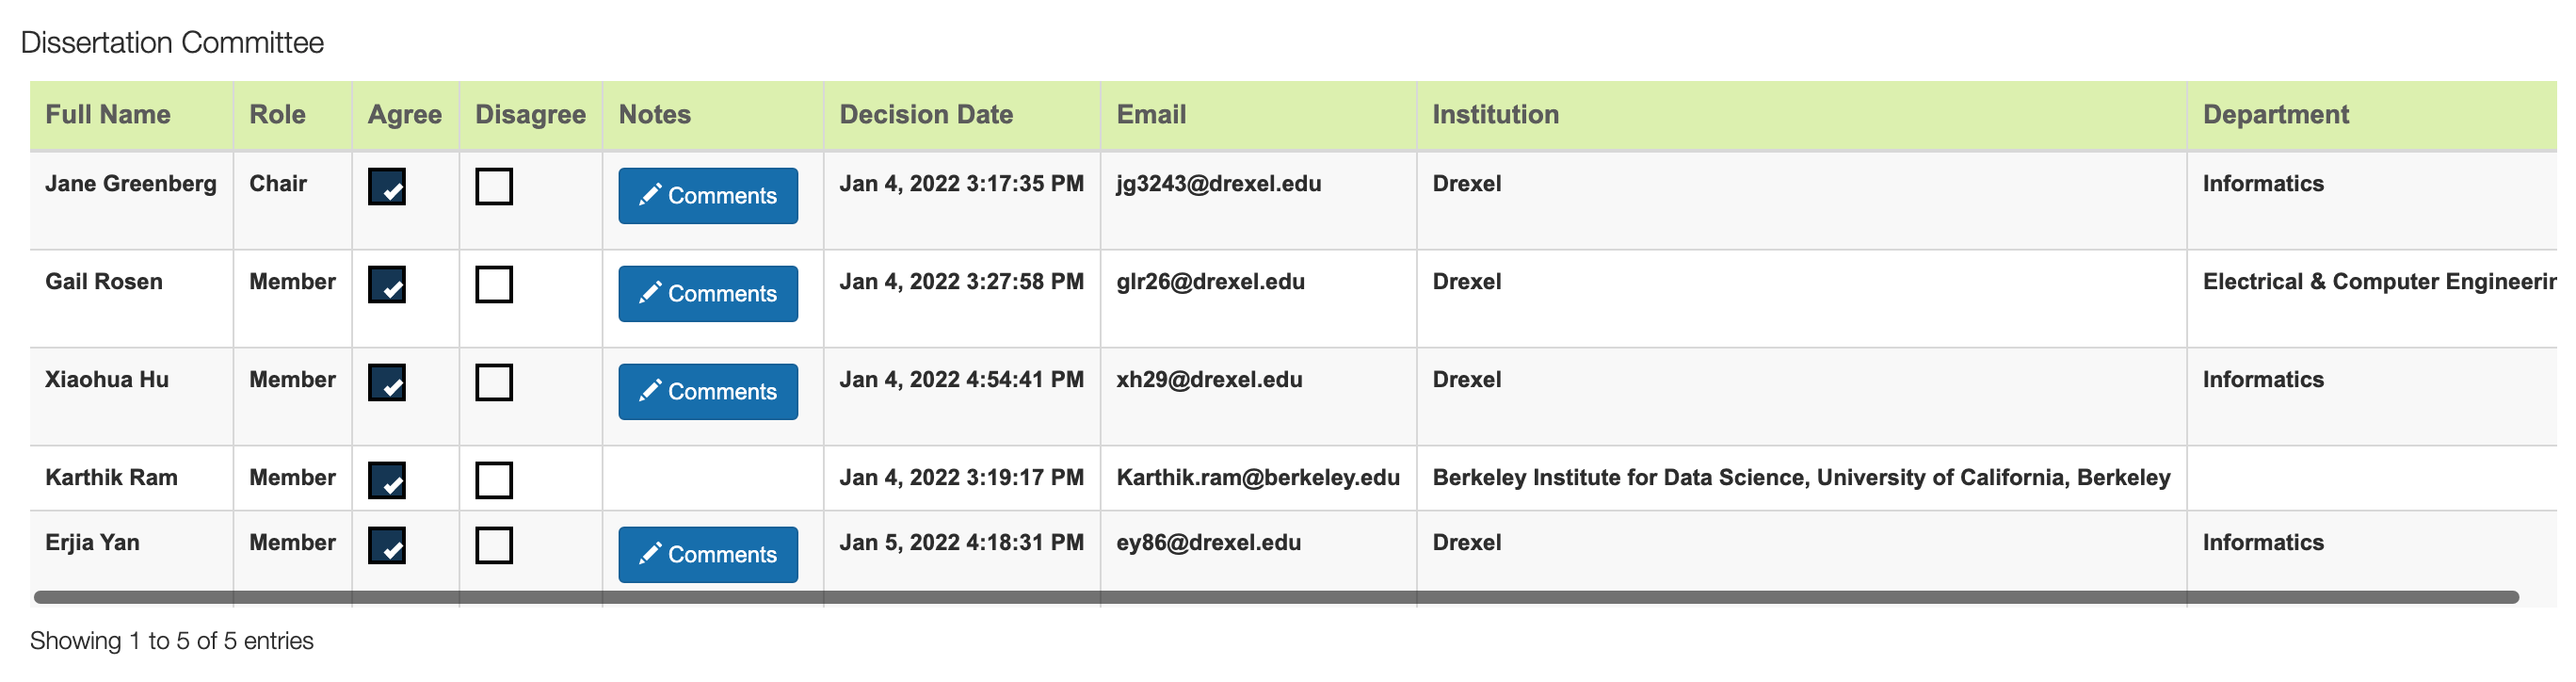
\includegraphics[width=\textwidth]{./images/signatureform.png}

\title{Tests of Robustness in Peer Review}
\date{}
\author{Jeremy Leipzig}
\degree{Doctor of Philosophy}
\gyear{2021}
\gmonth{December}
\degreearea{Information Science}

\advisor{Jane Greenberg, PhD}
\advisor{Karthik Ram, PhD}
\advisor{Gail Rosen, PhD}
\advisor{Xiaohua Tony Hu, PhD}
\advisor{Erjia Yan, PhD}

\maketitle

\copyrightpage


{\Large Acknowledgments}

I am deeply indebted to my wife Mary Ellen McCarty for her support and sacrifices during this long journey. My mother Pat Ward was also a great help to me.

I wish to thank my patient and calm advisor, Jane Greenberg, the thesis committee - Karthik Ram, Gail Rosen, Xiaohua Tony Hu, Erjia Yan - and Chamoei Chen, who suggested I write the pipeline paper.

My work in this dissertation originated from my exposure to the brilliant statistician Charles Berry, who introduced me to reproducible research in 2004. I am also grateful to Frederic Bushman, who brought me in touch with Dr. Berry, and to my master's advisor Steffen Heber, who recommended me to Dr. Bushman.

I am thankful to CHOP for funding a portion of the tuition and providing much of the experiential fodder for this unusual research topic. Many of the reproducibility frustrations of working in a large research organization were made more bearable by my past colleagues - Deanne Taylor, Zhe Zhang, Perry Evans, Komal Rathi, Pichai Raman, and Eric Lim.

Throughout this dissertation, I received valuable contributions from Sandeep Amberkar, Stephen Anderson, Israel Barrantes, Juan Caballero, Barry Digby, Harish K, Charlie Lonergan, Ammar Naqvi, Daniel Nüst, Wade Rogers, Yi Xing, and Karl Sebby.


{\Large Declaration}

This dissertation is the result of my own work, except where explicit reference is made to the work of others. It has not been submitted for another qualification to this or any other university. This dissertation does not exceed the word limit for the respective Degree Committee.

\newpage
\tableofcontents

\listoftables

\listoffigures



\clearpage
\newpage 


{\Large Abstract}

\uline{Purpose}: The purpose of this dissertation is to investigate the feasibility of using tests of robustness in peer review. This study involved selecting three high-impact papers which featured open data and utilized bioinformatic analyses but provided no source code and refactoring these to allow external survey participants to swap tools, parameters, and data subsets to evaluate the robustness and underlying validity of these analyses. Technical advances that have taken place in recent years - scientific computing infrastructure has matured to support the distribution of reproducible computational analyses - enable this approach. These advances, along with cultural shifts encompassing open data and open code initiatives, promise to address technical stumbling blocks that have contributed to the "reproducibility crisis." To take full advantage of these developments toward improving scientific quality, authors, reviewers, and publishers must integrate reproducible analysis into the peer review process. Seven existing major case study types - reproduction, replication, refactor, robustness test, survey, census, and case narrative - have been invaluable toward establishing reproducibility as a serious and independent area of research. Of particular interest are refactors, in which an existing analysis with abstract methods is reimplemented by a third party, and robustness tests, which involve the manipulation of tools, parameters, and data to assess the scientific validity of an analysis. This thesis describes efforts to test the feasibility of robustness testing in the context of in silico peer review. The contributions described are complemented with extensive source code.

\uline{Design and Methods}: A multi-method approach was employed for this study consisting of user surveys and tests of robustness - hands-on, self-directed software development exercises. Three high-impact genomics publications with open data, but no source code, were selected, refactored, and distributed to active study participants who acted as quasi-external reviewers. The process of the refactor was used to evaluate the limitations of reproducibility using conventional tools and to study how best to present analyses for peer review, and the tests of robustness were employed under the hypothesis this practice would help to evaluate the underlying validity of an analysis. Three different approaches were taken in these tests of robustness - a faithful reproduction of the original manuscript into a framework that could be manipulated by participants, a workflow-library approach in which participants were encouraged to employ modern "off-the-shelf" pre-built pipelines to triangulate tests, and an advisor-led approach in which senior experts suggested alternate tools to be implemented and I generated a report for their evaluation. 

\uline{Findings}: The refactors and tests of robustness produced numerous discoveries both in terms of the underlying scientific content and, more importantly, into the strengths and weakness of the three robustness approaches (faithful/workflow-library/advisor-led) and pain points in the analytic stack, which may be addressed with appropriate software and metadata. The principal findings are that the faithful approach may often discourage aggressive robustness testing because of the inertia imposed by the existing framework, the workflow-library approach is efficient but can prove inconclusive, and the advisor-led approach may be most practical for journals but requires a higher level of communication to be effective. The vast majority of time in all these refactors was spent on sample metadata management, particularly organizing sample groups of biological and technical replicates to produce the numerous and varied tool input manifests. 

\uline{Practical Implications}: Reproducibility-enabled in silico peer review is substantially more time-consuming than traditional manuscript peer review and will require economic, cultural, and technical change to bring to reality. The work presented here could contribute to developing new models to minimize the increased effort of this type of peer review while incentivizing reproducibility.

\uline{Value}: This study provides practical guidance toward designing the future of reproducibility-enabled in silico peer review, which is a logical extension of the computational reproducibility afforded by technical advances in dependency management, containerization, pipeline frameworks, and notebooks.

\newpage 

\ % The empty page

\newpage

\section{Introduction}

In recent years, various fields - namely the biomedical sciences, psychology, and neuroscience, but also newer areas such as artificial intelligence - have decried a "reproducibility crisis" \cite{Baker2016-ri} in the form of unreproducible analyses or unreplicable results. The primary origins of these problems are selective reporting and insufficient detail provided in methods, which can include missing code, data, versions, or parameters. These details encompass all steps of the scientific endeavor, from laboratory protocols, data collection, data processing, analysis, and manuscript editing.

Reproducible research is not yet a formally established area of study or curricula in information science, despite increasing attention within an array of scientific fields and as a primary focus of several researchers, institutions, and journals. Only one dissertation exists with a title bearing the phrase "reproducible research" or "reproducible computational research" \cite{Pham2014-ad}. The field of information science, straddling the fence between computer science and its applied domains, is uniquely positioned to accommodate reproducible computational research as a topic of study in its own right. This proposal intends to serve as a progenitor for this new subdomain by exploring metadata as a syntactic glue to bind layers of the "analytic stack."

\subsection{Reproducible Research}

Reproducible Research is an umbrella term that encompasses many forms of scientific quality - from generalizability of underlying scientific truth, an exact recreation of an experiment with or without communicating intent, to the open sharing of analysis for reuse. Specific to computational facets of scientific research, Reproducible Computational Research (RCR)\cite{Donoho2010-xp} encompasses all aspects of in silico analyses, from the propagation of raw data collected from the experimental lab, field, or instrumentation, through intermediate data structures. computational hardware, to open code and statistical analysis, and finally publication. Reproducible research points to several underlying concepts of scientific validity – terms that should be unpacked to be understood. Stodden et al. \cite{Stodden2013-ce} devised a five-level hierarchy of research, classifying it as – reviewable, replicable, confirmable, auditable, and open or reproducible. Whitaker \cite{Whitaker2016-gl} describes an analysis as "reproducible" in the narrow sense that a user can produce identical results provided the data and code from the original, and "generalisable" if it produces similar results when both data is swapped out for similar data ("replicability"), and if underlying code is swapped out with comparable replacements ("robustness") (Figure \ref{whitaker}). 

\begin{figure}[h!]
	\centering
	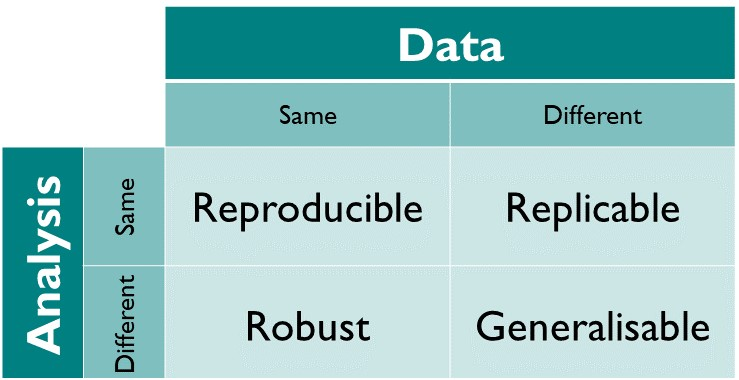
\includegraphics[width=11.65cm,height=6.01cm]{./images/whitaker.png}
	\caption{Whitaker's matrix of reproducibility \cite{The_Turing_Way_Community2019-fn}}
	\label{whitaker}
\end{figure}

While these terms may confuse those new to reproducibility, a review by Barba disentangled the terminology while providing a historical context of the field \cite{Barba2018-qv}. One major conflicted use of terms (reproducible/replicable) has since then been harmonized \cite{noauthor_undated-or}.  A wider perspective places reproducibility as a first-order benefit of applying FAIR principles: Findability, Accessibility, Interoperability, and Reusability \cite{Wilkinson2016-qr}.

Reproducible computational research (the "reproducible" in Whitaker's table) is attainable with current technology with a few caveats - namely external resources and manual steps. There is some debate whether implementing reproducibility is "still a challenge" \cite{FitzJohn2014-wk}  or "not hard" \cite{Edzer_Pebesma2016-gl}. The tools to achieve highly portable and automated analyses such as Conda, Docker, cloud computing, pipeline frameworks, notebooks, and script provenance tools are readily available, even if some are quite new. 

RCR is necessary but not sufficient to achieve the other three types of reproducibility (replicability, robustness, and generalizability). It is impossible to evaluate the replication (swapping in new data) or robustness (swapping in new tools) of a complex computational workflow if it is not first reproducible. Those types of reproducibility rely on some level of scientific validity (i.e., truth) to realize. Methods to measure replicability, robustness, and generalizability are also indirectly measuring the strength of scientific hypotheses rather than best practices in reproducible research. As mentioned above, a binary condemnation of "Not replicable" might infer a scientific result is not valid when the infraction might be relatively minor - for example, a missing but ultimately derivable parameter. Conversely, a highly transparent and automated analysis can still suffer from design problems and small sample sizes that can lead to artefactual results. The Begley and Ellis Amgen study cited poor design, poor statistics, and perhaps most commonly, selective reporting, rather than record-keeping or lack of lab notebooks as the primary factor in a failure to validate \cite{Begley2012-mt}. This contrasts somewhat with the Ioannidis microarray review discussed above \cite{Ioannidis2009-at}, which identified most reproducibility problems as being due to a lack of detailed methods, missing controls, and other failures in protocol.

Munafò and Smith contend that the four types of reproducibility cited by Whitakerare not sufficient to verify scientific validity because they do not eliminate common confounders. They posit that \textit{triangulation}, defined as applying entirely different approaches (each with differing biases) and multiple lines of evidence to the same problem, is a more appropriate use of resources.\cite{noauthor_undated-xz} 

Millman and colleagues in "Is tagging of therapist-patient interactions reliable?" \cite{jarrod} classify reproducibility into four categories. 

\begin{itemize}
	\item Computational reproducibility and transparency

	\item Scientific reproducibility and transparency

	\item Computational correctness

	\item Statistical reproducibility

\end{itemize}
These divisions correspond to the divides between reproducibility/replicability and between wet-lab and \textit{in silico} analysis.

\subsubsection{Secondary Attributes of Reproducibility}

Building on those primary types are nine secondary attributes of manuscript reproducibility, perhaps best described by Stodden - replicable, reproducible, repeatable, confirmable, generalizable, reviewable, auditable, verifiable, and validatable. Many of these attributes revolve around the free and unrestricted availability of data. As a tenet or a prerequisite to reproducibility, the role of open data and the open data movement is a lengthy topic by itself but also affects the standards and means of measuring reproducibility. The data-sharing movement - including Open Access and FAIR \cite{Wilkinson2016-qr}-- has developed somewhat tangentially to the reproducibility movement, although these share many of the same values of reuse, evaluation, and scientific validity. In biomedical science, open data is largely driven by the need to reach a critical mass of patient data to derive statistical power, especially in rare disease. Sample sizes in the thousands are often necessary to utilize machine learning techniques. "Deep learning" requires even more. In data science, open data is often associated with larger social and political government transparency issues.

The reproducibility movement can be presented as an "open analysis" (as opposed to "open data") movement. However, this characterization oversimplifies both the challenges of creating reproducible workflows in terms of portability, transparency and other characteristics in the same way "open data" glosses over some of the finer points of tidiness and metadata.

Rokem, Marwick, and Steneva \cite{Marwick2017-ie} classify the three facets of reproducibility as

\begin{itemize}
	\item Automation and provenance tracking - includes the single-button press criteria

	\item Availability of software and data

	\item Open reporting of results

\end{itemize}
\subsubsection{Tertiary Attributes of Reproducibility}

Finally, quality attributes are associated with reproducibility in a tangential fashion, most often connected with software engineering and information and library science.  

\paragraph{Attributes from software engineering}

The computational reproducibility community is closely aligned with computer science and software development communities, which have developed various software engineering habits,  development methodologies, best practices, and standards that may embody these high-level qualitative characteristics, engendering "checklist"-style rubrics. These include version control, provenance tracking (tracing the origins of data and intermediates), documentation, pipeline frameworks, and continuous integration \cite{Sandve2013-yv,Noble2009-ad}. Most of the concepts here have been directly borrowed from research in industrial software engineering settings \cite{Losavio2004-tg,Technology2003-gl}, and many have formal software quality ISO9126 entries.

\begin{itemize}
	\item Automation - Are there checkpoints that require human judgment to proceed, either because a machine learning or other automated routine has not yet been developed or because there are steps that involve web applications, desktop software, or other interactive tools which disrupt flow?

	\item Swappability - Refers to how readily can alternative tools and analytical steps be replaced with substitutes. This is incredibly important for testing whether a result is an artifact created by a particular tool or model. In software quality terms, this is referred to as ISO 9126 Maintainability Sub-characteristic Replaceability

	\item Modularity - can individual tools, steps, and reports be extracted and used by others. Maintainability Sub-characteristic Modularity 

	\item Discoverability - how readily is this project going to be found by others, even those in a different field but whose workflow resembles the project 

	\item Readability - is source code well enough documented to be inspected and understood by programmers familiar with the tool but unfamiliar with the underlying implementation.

	\item Abstracted - does the project use conventional standard frameworks, such as pipeline frameworks - either CWL-based or a DSL\cite{Leipzig2017-hv}. 

	\item Portability - can the software dependencies of an analysis be seamlessly installed on a different server? Are they specified in a server-agnostic dependency manager such as Conda? Are Docker \cite{Schulz2016-or} or Singularity containers \cite{Kurtzer2017-wb} used to isolate individual processes? Is the infrastructure "cloud-ready"?

	\item Uncoupledness - is the software designed as a loosely coupled service-oriented architecture that leverages application programming interfaces (APIs), preferably in a stateless or RESTful web interface. A popular framework for such services is Swagger \cite{Haupt2017-ud}. For more highly linked data, a SPARQL endpoint may be preferable.\cite{Gonzalez2014-dq}

	\item Scalability - can a process be configured to use multiple cores, multiple nodes, batch submission systems, or more sophisticated big data shared memory frameworks such as Spark.

	\item Loggability - does the workflow record steps during progression?

	\item Monitoring - can the workflow be monitored in real-time?

	\item Tested - have tests been developed? Are there test coverage statistics?

	\item Debuggability - can bugs in the project be easily identified? Is continuous integration used?

	\item Updatability - can the project be updated with new resources?

	\item Extensibility - can one easily build on an analysis to suit a different experimental design?

	\item Robustness - can the software work in a variety of contexts?

	\item Gracefulness - can the software handle exceptions and report meaningful errors?

	\item Defensiveness - does the software detect error states early on?

	\item Reentrancy and memoization - can a workflow be restarted where it left off if interrupted? Can a downstream target deliverable be produced from intermediates?

\end{itemize}
\paragraph{Attributes from information science}

Another facet of RCR research is provided by researchers in information and library science. These include the following attributes:

\begin{itemize}
	\item Semantic encoding  - semantic data contains markup, metadata that defines the meaning of data for computation, discovery, reuse, and attribution. Metadata is essential for the wet-lab technical, computational, scientific, and bibliographic layers of a research project.

	\item Metadata - are data dictionaries used? Are the Dublin Core elements complete?

	\item Linkedness - Are standards for linked metadata used to provide means of unambiguous identification with uniform resource identifiers? Are resource description frameworks leveraged to enable the relationship between entities to be defined using standard ontologies? Research objects \cite{Bechhofer2010-lr} provide a framework for tying together the data, code, workflows, and publications related to a project using a standard ontology.

	\item Provenance - are the origins of data properly recorded? \cite{Herschel2017-yc}

	\item Sustainability - are sustainable and permanent data identifiers employed? \cite{Gomez-Perez2013-th,Zhao2012-ou}. Are external databases or files cached such that the version used is available?

\end{itemize}
\paragraph{Attributes from statistics and data science}

Statistics and data science have introduced key attributes of report-level reproducibility:

\begin{itemize}
	\item Tidiness - is the raw input data munged into a format that conforms to tidy data standards as described by Hadley Wickham \cite{Wickham2014-xj}. Tidy data tends to be "tall," rather than "wide," with value classifier variables as row values rather than column headings, and only one observation or measurement, all of the same data type, appears in each row.

	\item Subsetability - can a project’s data be easily subset or randomly sampled for cross-validation?

	\item Literacy - the statistical code is interspersed with contextual text that describes the intent of each block.

	\item Prospective stability - the model, operation, or algorithm can map new data points without affecting existing results.

\end{itemize}
No word or phrase encompasses all of the attributes above to the author's knowledge. One possible term would be "broad-sense reproducibility" (BSR), which I use to describe  "narrow-sense RCR" (aka "hit return reproducibility" - the ability to execute a packaged analysis with little effort) with the added goals of discovery, reuse, and transparency in line with Findable, Accessible, Interoperable, and Reusable (FAIR) principles \cite{Wilkinson2016-qr}. A recent effort to develop metrics for FAIR has emphasized a rubric that is "clear", "realistic", "discriminating", "measurable", and "universal" \cite{Wilkinson2017-hf}

\subsubsection{Reproducibility Crisis}

The scientific community’s challenge with irreproducibility in research has been extensively documented \cite{Baker2016-ri}. Two events in the life sciences stand as watershed moments in this crisis – the publication of manipulated and falsified predictive cancer therapeutic signatures by a biomedical researcher at Duke and subsequent forensic investigation by Keith Baggerly and David Coombes \cite{Baggerly2010-qy}, and a review by scientists at Amgen who could replicate the results of only 6 out of 53 cancer studies \cite{Begley2012-mt}. These events involved different aspects of research practice - poor data structures and missing protocols, respectively. Together with related studies \cite{Ioannidis2009-at}, they underscore recurring reproducibility problems due to a lack of detailed methods, missing controls, and other protocol failures, including inappropriate statistical tests and or misinterpretation of results, also play a recurring role in irreproducibility \cite{Motulsky2014-vg}. Regardless of intent, these activities fall under the umbrella term of "questionable research practices." It bears speculation whether these types of incidents are more likely to occur in novel statistical or computational approaches compared to conventional ones. Subsequent surveys of researchers \cite{Baker2016-ri} have identified selective reporting, while theory papers \cite{Ioannidis2005-se} have emphasized the insidious combination of underpowered designs and publication bias, essentially a multiple testing problem on a global scale. We contend that metadata has been undervalued in the role it can play in addressing all of these issues and shifting the narrative from the current crisis to new opportunities \cite{Fanelli2018-ek}.

In the wake of this newfound interest in reproducibility, both the variety and volume of related case studies increased after 2015 (Figure 2). Likert-style surveys and high-level publication-based censuses (see Figure 3) in which authors tabulate data or code availability are most prevalent. Additionally, low-level reproductions, in which code is executed, replications in which new data is collected and used, tests of robustness in which new tools or methods are used, and refactors to best practices are also becoming more popular. While the life sciences have generated more than half of these case studies, areas of the social and physical sciences are increasingly the subjects of important reproduction and replication efforts. 

The majority of studies into reproducible research have focused on the first row of Whitaker's grid and replication in particular. The reasons for this bias are most perhaps rooted in how science has typically been conducted in those areas that have experienced the most public reproducibility crises - psychology and the life sciences  - where generating new data to test existing hypotheses is more common than modeling existing datasets, as is more common in the physical sciences.

\subsubsection{Big Data, Big Science, and Open Data}

The inability of third parties to reproduce results is not new to science \cite{Lehrer2010-pm}, but the scale of scientific endeavor and the level of data and method reuse suggest replication failures may damage the sustainability of certain disciplines, hence the term "reproducibility crisis." The problem of irreproducibility is compounded by the rise of "big data," in which very large, new, and often unique, disparate or unformatted sources of data have been made accessible for analysis by third parties, and "big science," in which terabyte-scale data sets are generated and analyzed by multi-institutional collaborative research projects on specialized and possibly unique infrastructure. Big data and big science have increased the demand for high-performance computing, specialized tools, and complex statistics, with attention to the growing popularity and application of machine learning and deep learning (ML/DL) techniques to these data sources. Such techniques typically train models on specific data subsets, and the models, as the end product of these methods, are often "black boxes," i.e., their internal predictors are not explainable (unlike older techniques such as regression) though they provide a good fit for the test data. Properly evaluating and reproducing studies that rely on such algorithms presents new challenges not previously encountered with inferential statistics \cite{Warden2018-ak,Bouthillier2019-yq}. Computational reproducibility is typically focused on the last analytic steps of what is often a labor-intensive scientific process that often originates from wet-lab protocols, fieldwork, or instrumentation, and these last in silico steps present some of the more difficult problems both from technical and behavioral standpoints, because of the amount of entropy introduced by the sheer number of decisions made by an analyst. This "decision entropy" is a possible contributor to many problems in replications, Hoffmann et al. state "there are concerns that this multiplicity of analysis strategies plays an important role in the non-replicability of research findings"\cite{Hoffmann2020-sb}. Ironically, these choices are also being utilized to evaluate the quality of science, which is the point of this dissertation.

The ability of third parties to reproduce studies relies on access to the raw data and methods employed by authors. Much to the exasperation of scientists, statisticians, and scientific software developers, the rise of "open data" has not been matched by "open analysis," as evidenced by several case studies \cite{Obels2019-sy,Rauh_undated-ej,Stodden2018-ls,Stagge2019-fv}.

Missing data and code can obstruct the peer review process, where proper review requires the authors to put forth the effort necessary to share a reproducible analysis. Software development practices, such as documentation and testing, are not a standard requirement of the doctoral curriculum, the peer-review process, or the funding structure – and as a result, the scientific community suffers from diminished reuse and reproducibility \cite{Nust2018-wx}. Sandve et al. \cite{Sandve2013-yv} identified the most common sources of these oversights in "Ten Simple Rules for Reproducible Computational Research" – lack of workflow frameworks, missing platform and software dependencies, manual data manipulation or forays into web-based steps, lack of versioning, lack of intermediates and plot data, and lack of literate programming or context can derail a reproducible analysis.

An issue distinct from the availability of source code and raw data is the lack of metadata to support reproducible research. We have observed many of the findings from case studies in reproducibility point to missing methods details in an analysis, which can include software-specific elements such as software versions and parameters \cite{Collberg2014-cj}, but also steps along the entire scientific process including data collection and selection strategies, data processing provenance including hardware, statistical methods and linking these elements to publication. We find the key concept connecting all of these issues is metadata.

An ensemble of dependency management and containerization tools already exist to accomplish narrow-sense reproducibility \cite{Piccolo2016-kd} – the ability to execute a packaged analysis with little effort from a third party. But context to allow for robustness and replicability, "broad-sense reproducibility," is limited without endorsement and integration of necessary metadata standards that support discovery, execution, and evaluation. Despite the growing availability of open-source tools, training, and better executable notebooks, reproducibility is still challenging \cite{FitzJohn_undated-bq}. The following sections address these issues by first defining metadata, defining an "analytic stack" to abstract the steps of an in silico analysis, and then identifying and categorizing standards both established and in development to foster reproducibility.

Overall, the review above documenting aspects of the reproducibility crisis underscores the need to investigate this topic from multiple perspectives to ameliorate further crises. The research presented below, first examining existing case studies, then implementing tests of robustness to explore their viability as a natural extension of peer review, seeks to address the reproducibility crisis in terms of critical and exploratory evaluation.

\subsubsection{Existing Methods in Reproducible Research Case Studies}

Surveys and censuses have provided a valuable understanding of the scope and nature of the reproducibility crisis. However, reproductions, refactors, and tests of robustness are most appropriate for in-depth investigations into reproducible computational research of the in silico variety. 

This dissertation seeks to leverage three existing case study approaches using a mixed-methods approach consisting of a \textit{refactor}, followed by a survey and a brief user testing exercise called a test of robustness. A \textit{refactor} is a type of case study used in reproducible research in which a study that is presumably valid but poorly reproducible is brought up to higher standards. A refactor one of several available approaches that have been used in this area. To survey the existing efforts of formal measurement, I collected 40 case studies on reproducible research. This is published on \href{https://github.com/leipzig/awesome-reproducible-research}{\uline{Awesome Reproducible Research}}, a crowdsourced curated list of reproducible research case studies, projects, tutorials, and media.

\newpage

\paragraph{Case Study Methodologies}

\begin{figure}[h!]
	\centering
	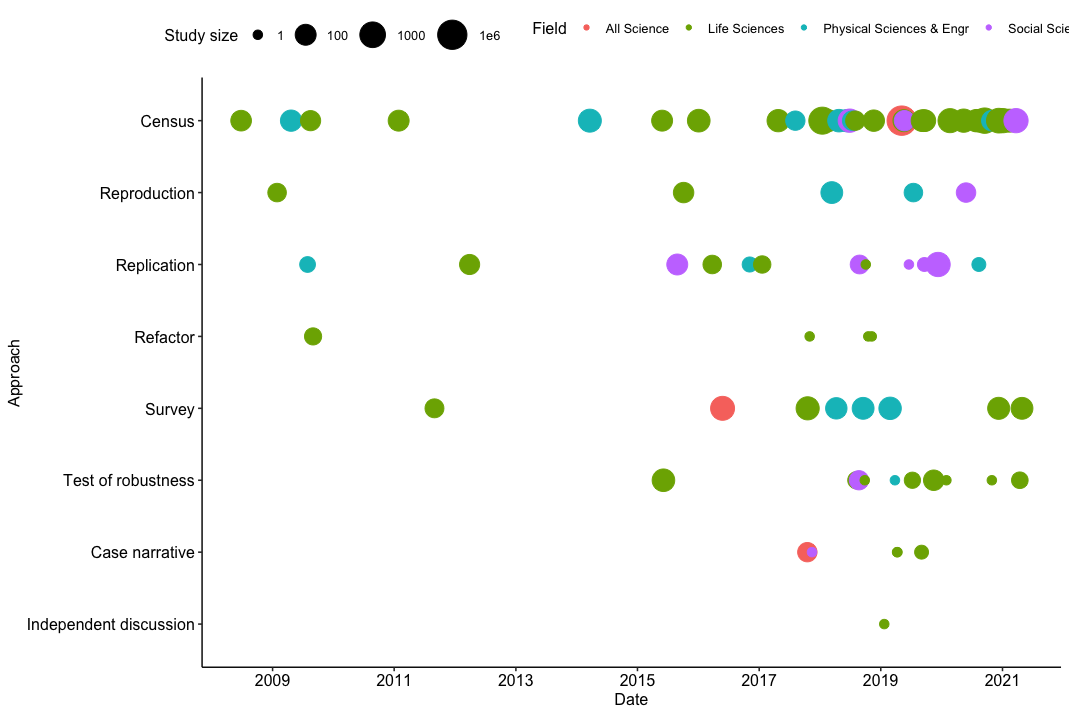
\includegraphics[width=\textwidth,height=11.04cm]{./images/casestudies.png}
	\caption{Timeline of case studies in reproducible research}
	\medskip
    \small
	The term "case studies" is used in a general sense to describe any study of reproducibility. A reproduction is an attempt to arrive at comparable results with identical data using computational methods described in a paper. A refactor involves refactoring existing code into frameworks and reproducible best practices while preserving the original data. A replication involves generating new data and applying existing methods to achieve comparable results. A test of robustness applies various protocols, workflows, statistical models, or parameters to a given dataset to study their effect on results. A census is a high-level tabulation conducted by a third party. A survey is a questionnaire sent to practitioners. A case narrative is an in-depth first-person account. An independent discussion utilizes a secondary independent author to interpret the results of a study as a means to improve inferential reproducibility. \cite{Leipzig2019-am}.
	\label{casestudies}
\end{figure}

\newpage
\begin{table}[H]
\begin{adjustbox}{max width=\textwidth}
\begin{tabular}{p{3.86cm}p{4.12cm}p{4.29cm}p{4.24cm}p{3.86cm}p{4.12cm}p{4.29cm}p{4.24cm}}
\multicolumn{1}{p{3.86cm}}{\textbf{Study}} & 
\multicolumn{1}{p{4.12cm}}{\textbf{Field}} & 
\multicolumn{1}{p{4.29cm}}{\textbf{Approach}} & 
\multicolumn{1}{p{4.24cm}}{\textbf{Size}} \\ 
\multicolumn{1}{p{3.86cm}}{Ioannidis 2005 \cite{Ioannidis2005-se}} & 
\multicolumn{1}{p{4.12cm}}{Science} & 
\multicolumn{1}{p{4.29cm}}{Theoretical} & 
\multicolumn{1}{p{4.24cm}}{(all studies)} \\ 
\multicolumn{1}{p{3.86cm}}{Glasziou et al. 2008 \cite{Glasziou2008-of}} & 
\multicolumn{1}{p{4.12cm}}{Medicine} & 
\multicolumn{1}{p{4.29cm}}{Census} & 
\multicolumn{1}{p{4.24cm}}{80 studies} \\ 
\multicolumn{1}{p{3.86cm}}{Baggerly $\&$ Coombes 2009 \cite{Baggerly2010-gt}} & 
\multicolumn{1}{p{4.12cm}}{Cancer biology} & 
\multicolumn{1}{p{4.29cm}}{Refactor} & 
\multicolumn{1}{p{4.24cm}}{8 studies} \\ 
\multicolumn{1}{p{3.86cm}}{Hothorn et al. 2009 \cite{Hothorn2009-sx}} & 
\multicolumn{1}{p{4.12cm}}{Biostatistics} & 
\multicolumn{1}{p{4.29cm}}{Census} & 
\multicolumn{1}{p{4.24cm}}{56 studies} \\ 
\multicolumn{1}{p{3.86cm}}{Ioannidis et al. 2009 \cite{Ioannidis2009-at}} & 
\multicolumn{1}{p{4.12cm}}{Genetics} & 
\multicolumn{1}{p{4.29cm}}{Reproduction} & 
\multicolumn{1}{p{4.24cm}}{18 studies} \\ 
\multicolumn{1}{p{3.86cm}}{Anda et al. 2009 \cite{Anda2009-lr}} & 
\multicolumn{1}{p{4.12cm}}{Software engineering} & 
\multicolumn{1}{p{4.29cm}}{Replication} & 
\multicolumn{1}{p{4.24cm}}{4 companies} \\ 
\multicolumn{1}{p{3.86cm}}{Vandewalle et al. 2009 \cite{Vandewalle2009-pe}} & 
\multicolumn{1}{p{4.12cm}}{Signal processing} & 
\multicolumn{1}{p{4.29cm}}{Census} & 
\multicolumn{1}{p{4.24cm}}{134 papers} \\ 
\multicolumn{1}{p{3.86cm}}{Prinz 2011 \cite{Prinz2011-ej}} & 
\multicolumn{1}{p{4.12cm}}{Biomedical sciences} & 
\multicolumn{1}{p{4.29cm}}{Survey} & 
\multicolumn{1}{p{4.24cm}}{23 PIs} \\ 
\multicolumn{1}{p{3.86cm}}{Horthorn $\&$ Leisch 2011 \cite{Hothorn2011-pb}} & 
\multicolumn{1}{p{4.12cm}}{Bioinformatics} & 
\multicolumn{1}{p{4.29cm}}{Census} & 
\multicolumn{1}{p{4.24cm}}{100 studies} \\ 
\multicolumn{1}{p{3.86cm}}{Begley $\&$ Ellis 2012 \cite{Begley2012-mt}} & 
\multicolumn{1}{p{4.12cm}}{Cancer biology} & 
\multicolumn{1}{p{4.29cm}}{Replication} & 
\multicolumn{1}{p{4.24cm}}{53 studies} \\ 
\multicolumn{1}{p{3.86cm}}{Collberg et al. 2014 \cite{Collberg2014-cj} \newline
Collberg $\&$ Proebsting 2016 \cite{Collberg2016-we}} & 
\multicolumn{1}{p{4.12cm}}{Computer science} & 
\multicolumn{1}{p{4.29cm}}{Census} & 
\multicolumn{1}{p{4.24cm}}{613 papers} \\ 
\multicolumn{1}{p{3.86cm}}{OSC 2015 \cite{Open_Science_Collaboration2015-rm}} & 
\multicolumn{1}{p{4.12cm}}{Psychology} & 
\multicolumn{1}{p{4.29cm}}{Replication} & 
\multicolumn{1}{p{4.24cm}}{100 studies} \\ 
\multicolumn{1}{p{3.86cm}}{Bandrowski et al. 2015 \cite{Bandrowski2015-qu}} & 
\multicolumn{1}{p{4.12cm}}{Biomedical sciences} & 
\multicolumn{1}{p{4.29cm}}{Census} & 
\multicolumn{1}{p{4.24cm}}{100 papers} \\ 
\multicolumn{1}{p{3.86cm}}{Patel et al. 2015 \cite{Patel2015-zu}} & 
\multicolumn{1}{p{4.12cm}}{Epidemiology} & 
\multicolumn{1}{p{4.29cm}}{Robustness test} & 
\multicolumn{1}{p{4.24cm}}{417 variables} \\ 
\multicolumn{1}{p{3.86cm}}{Névéol et al. 2016 \cite{Neveol2016-ou}} & 
\multicolumn{1}{p{4.12cm}}{NLP} & 
\multicolumn{1}{p{4.29cm}}{Replication} & 
\multicolumn{1}{p{4.24cm}}{3 studies} \\ 
\multicolumn{1}{p{3.86cm}}{Reproducibility Project 2017 \cite{Nosek2017-jk}} & 
\multicolumn{1}{p{4.12cm}}{Cancer biology} & 
\multicolumn{1}{p{4.29cm}}{Replication} & 
\multicolumn{1}{p{4.24cm}}{9 studies} \\ 
\multicolumn{1}{p{3.86cm}}{Vasilevsky et al. 2017 \cite{Vasilevsky2017-vd}} & 
\multicolumn{1}{p{4.12cm}}{Biomedical sciences} & 
\multicolumn{1}{p{4.29cm}}{Census} & 
\multicolumn{1}{p{4.24cm}}{318 journals} \\ 
\multicolumn{1}{p{3.86cm}}{Kitzes et al. 2017 \cite{Kitzes2017-qx}} & 
\multicolumn{1}{p{4.12cm}}{Science} & 
\multicolumn{1}{p{4.29cm}}{Case narrative} & 
\multicolumn{1}{p{4.24cm}}{31 PIs} \\ 
\multicolumn{1}{p{3.86cm}}{Barone et al. 2017 \cite{Barone2017-ac}} & 
\multicolumn{1}{p{4.12cm}}{Biological sciences} & 
\multicolumn{1}{p{4.29cm}}{Survey} & 
\multicolumn{1}{p{4.24cm}}{704 PIs} \\ 
\multicolumn{1}{p{3.86cm}}{Kim $\&$ Dumas 2017 \cite{Kim2017-rz}} & 
\multicolumn{1}{p{4.12cm}}{Bioinformatics} & 
\multicolumn{1}{p{4.29cm}}{Refactor} & 
\multicolumn{1}{p{4.24cm}}{1 study} \\ 
\multicolumn{1}{p{3.86cm}}{Camerer 2017 \cite{Camerer2016-tr}} & 
\multicolumn{1}{p{4.12cm}}{Economics} & 
\multicolumn{1}{p{4.29cm}}{Replication} & 
\multicolumn{1}{p{4.24cm}}{18 studies} \\ 
\multicolumn{1}{p{3.86cm}}{Olorisade 2017 \cite{Olorisade2017-wt}} & 
\multicolumn{1}{p{4.12cm}}{Machine learning} & 
\multicolumn{1}{p{4.29cm}}{Census} & 
\multicolumn{1}{p{4.24cm}}{30 studies} \\ 
\multicolumn{1}{p{3.86cm}}{Strupler $\&$ Wilkinson 2017 \cite{Strupler2017-rm}} & 
\multicolumn{1}{p{4.12cm}}{Archaeology} & 
\multicolumn{1}{p{4.29cm}}{Case narrative} & 
\multicolumn{1}{p{4.24cm}}{1 survey} \\ 
\end{tabular}
\end{adjustbox}
\end{table}
\begin{table}[H]
\begin{adjustbox}{max width=\textwidth}
\begin{tabular}{p{3.86cm}p{4.12cm}p{4.29cm}p{4.24cm}p{3.86cm}p{4.12cm}p{4.29cm}p{4.24cm}}
\multicolumn{1}{p{3.86cm}}{Danchev et al. 2017 \cite{Danchev2018-wf}} & 
\multicolumn{1}{p{4.12cm}}{Toxicogenomics} & 
\multicolumn{1}{p{4.29cm}}{Census} & 
\multicolumn{1}{p{4.24cm}}{51,292 claims in 3,363 papers} \\ 
\multicolumn{1}{p{3.86cm}}{Kjensmo $\&$ Gundersen 2017 \cite{Kjensmo2017-ni}} & 
\multicolumn{1}{p{4.12cm}}{Artificial intelligence} & 
\multicolumn{1}{p{4.29cm}}{Census} & 
\multicolumn{1}{p{4.24cm}}{400 papers} \\ 
\multicolumn{1}{p{3.86cm}}{Gertler et al. 2018 \cite{Gertler2018-uf}} & 
\multicolumn{1}{p{4.12cm}}{Economics} & 
\multicolumn{1}{p{4.29cm}}{Census} & 
\multicolumn{1}{p{4.24cm}}{203 papers} \\ 
\multicolumn{1}{p{3.86cm}}{Stodden et al. 2018 \cite{Stodden2018-oe}} & 
\multicolumn{1}{p{4.12cm}}{Computational science} & 
\multicolumn{1}{p{4.29cm}}{Reproduction} & 
\multicolumn{1}{p{4.24cm}}{204 articles, 180 authors} \\ 
\multicolumn{1}{p{3.86cm}}{Madduri et al. 2018 \cite{Madduri2018-kc}} & 
\multicolumn{1}{p{4.12cm}}{Genomics} & 
\multicolumn{1}{p{4.29cm}}{Case narrative} & 
\multicolumn{1}{p{4.24cm}}{1 study} \\ 
\multicolumn{1}{p{3.86cm}}{Camerer et al. 2018 \cite{Camerer2016-tr}} & 
\multicolumn{1}{p{4.12cm}}{Social sciences} & 
\multicolumn{1}{p{4.29cm}}{Replication} & 
\multicolumn{1}{p{4.24cm}}{21 papers} \\ 
\multicolumn{1}{p{3.86cm}}{Silberzahn et al. 2018 \cite{Silberzahn2015-yx}} & 
\multicolumn{1}{p{4.12cm}}{Psychology} & 
\multicolumn{1}{p{4.29cm}}{Robustness test} & 
\multicolumn{1}{p{4.24cm}}{One data set, 29 analyst teams} \\ 
\multicolumn{1}{p{3.86cm}}{Eaton et al. 2018 \cite{Eaton2018-gj}} & 
\multicolumn{1}{p{4.12cm}}{Microbiome immuno oncology} & 
\multicolumn{1}{p{4.29cm}}{Replication} & 
\multicolumn{1}{p{4.24cm}}{1 paper} \\ 
\multicolumn{1}{p{3.86cm}}{Vaquero-Garcia et al. 2018 \cite{Vaquero-Garcia2018-ax}} & 
\multicolumn{1}{p{4.12cm}}{Bioinformatics} & 
\multicolumn{1}{p{4.29cm}}{Refactor and test of robustness} & 
\multicolumn{1}{p{4.24cm}}{1 paper} \\ 
\multicolumn{1}{p{3.86cm}}{Wallach et al. 2018 \cite{Wallach2018-rk}} & 
\multicolumn{1}{p{4.12cm}}{Biomedical Sciences} & 
\multicolumn{1}{p{4.29cm}}{Census} & 
\multicolumn{1}{p{4.24cm}}{149 papers} \\ 
\multicolumn{1}{p{3.86cm}}{\href{https://drive.google.com/drive/folders/1thtenK7azxzys__RBH4ql3Y-x2J4OW-x}{\uline{Miller et al. 2018}} } & 
\multicolumn{1}{p{4.12cm}}{Bioinformatics} & 
\multicolumn{1}{p{4.29cm}}{Synthetic replication $\&$ refactor} & 
\multicolumn{1}{p{4.24cm}}{1 paper} \\ 
\multicolumn{1}{p{3.86cm}}{Konkol et al. 2018 \cite{Konkol2019-ld}} & 
\multicolumn{1}{p{4.12cm}}{Geosciences} & 
\multicolumn{1}{p{4.29cm}}{Survey, Reproduction} & 
\multicolumn{1}{p{4.24cm}}{146 scientists, 41 papers} \\ 
\multicolumn{1}{p{3.86cm}}{AlNoamany $\&$ Borghi 2018 \cite{AlNoamany2018-vh}} & 
\multicolumn{1}{p{4.12cm}}{Science $\&$ Engineering} & 
\multicolumn{1}{p{4.29cm}}{Survey} & 
\multicolumn{1}{p{4.24cm}}{215 participants} \\ 
\multicolumn{1}{p{3.86cm}}{Stagge et al. 2019 \cite{Stagge2019-fv}} & 
\multicolumn{1}{p{4.12cm}}{Geosciences} & 
\multicolumn{1}{p{4.29cm}}{Survey} & 
\multicolumn{1}{p{4.24cm}}{360 papers} \\ 
\multicolumn{1}{p{3.86cm}}{Bizzego et al. 2019 \cite{Bizzego2019-ij}} & 
\multicolumn{1}{p{4.12cm}}{Deep learning} & 
\multicolumn{1}{p{4.29cm}}{Robustness test} & 
\multicolumn{1}{p{4.24cm}}{1 analysis} \\ 
\multicolumn{1}{p{3.86cm}}{Madduri et al. 2019 \cite{Madduri2018-kc}} & 
\multicolumn{1}{p{4.12cm}}{Genomics} & 
\multicolumn{1}{p{4.29cm}}{Case narrative} & 
\multicolumn{1}{p{4.24cm}}{1 analysis} \\ 
\multicolumn{1}{p{3.86cm}}{Mammoliti et al. 2019 \cite{Mammoliti2019-ht}} & 
\multicolumn{1}{p{4.12cm}}{Pharmacogenomics} & 
\multicolumn{1}{p{4.29cm}}{Case narrative} & 
\multicolumn{1}{p{4.24cm}}{2 analyses} \\ 
\end{tabular}
\end{adjustbox}
\caption{Table of case studies in reproducible research}
\end{table}

\paragraph{Systematic Runnability Tests}

Several groups have begun to formalize the development of systematic in silico reproducibility tests, distinct from individual case studies or larger replication efforts such as the Open Science Framework Reproducibility Project. Software-based testing challenges such as CODECHECK \cite{Eglen2019-qm} focus on runnability, whereby a "code checker" certifies the code submitted with a paper executes on cloud-based infrastructure and produces outputs roughly identical to those in the paper, allowing for some leeway in terms of visible figures. ReScience is a peer-reviewed journal that targets computational replications \cite{Rougier2017-ys}. Rigorous reproducibility standards for submissions to NeurIPS have also been institutionalized \cite{Pineau2020-bs}. Despite the new opportunities afforded by reproducibility standards, and open data/open code, none of these tests typically involve the manipulation of tools or parameters. In the following sections, more involved techniques are discussed: refactoring and tests of robustness.

\begin{figure}[h!]
	\centering
	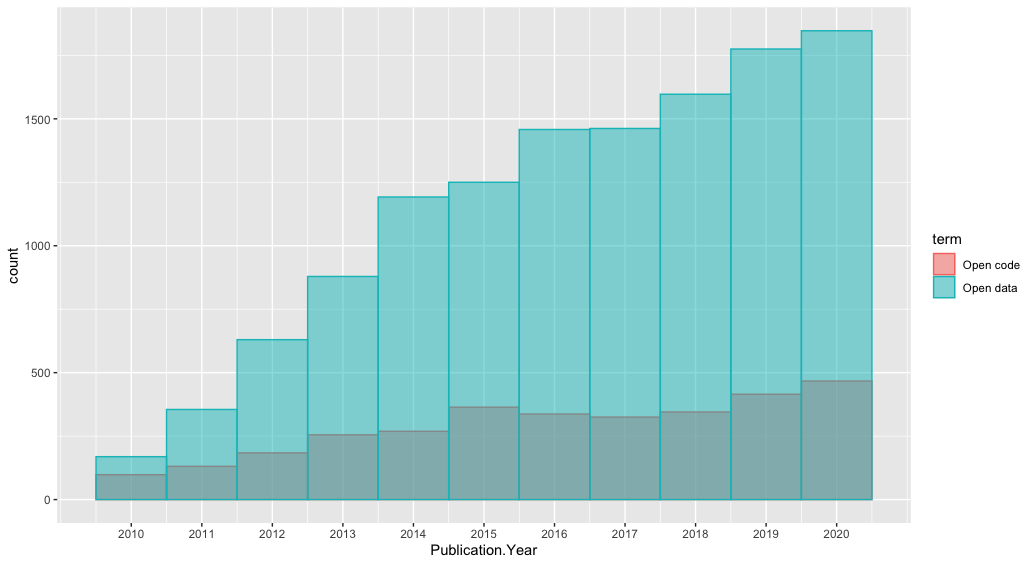
\includegraphics[width=13.76cm,height=7.47cm]{./images/odoc.png}
	\caption{Instances of the terms "open data" and "open code" in all abstracts 2010-2020}
	\medskip
\small
These terms point to necessary prerequisites for most approaches to reproducibility-enabled peer review
	\label{odoc}
\end{figure}

\subsubsection{Refactoring}

A reproduction can merely be as perfunctory as running someone else's code on their data, with no regard to other qualities of the code itself. A reproduction by its very nature assumes the paper is easily reproducible. A refactor involves an attempt to improve the broad-sense reproducibility of a study to a level higher than its initial state. Broad sense reproducibility is defined as the ability to execute a packaged analysis with little effort (narrow-sense) with the added goals of discovery, reuse, and transparency in line with Findable, Accessible, Interoperable, and Reusable (FAIR) principles \cite{Wilkinson2016-qr}. A recent effort to develop metrics for FAIR has emphasized a rubric that is "clear", "realistic", "discriminating", "measurable", and "universal" \cite{Wilkinson2017-hf}

A refactor is an appropriate initial approach for this dissertation for three reasons. First, a refactor enables an evaluation of key reproducibility fixtures including workflows, literate programming, and metadata standards. Second, A refactor enables the modularization and parameterization of tools and steps in a workflow to easily enable tests of robustness, in which a similar tool is substituted or the parameter landscape is explored to examine the robustness of the p-value or result being posited. A recent paper by Vaquero from the laboratory of Barash explores the refactoring aspect by swapping out both tool versions and data in a replication of an existing RNA splicing study \cite{Vaquero-Garcia2018-ax}. Finally, analyses, even more than data processing, involve numerous choices about appropriate statistical tests, dealing with outliers and missing data, normalization, correction for multiple comparisons, null and full models. An interesting study by Silberzahn et al. examined the various routes a statistical analysis could take by distributing a fixed data set of soccer official interactions and player variables to 29 teams, each charged with determining whether soccer referees are more likely to give red cards to dark-skin-toned players than to light-skin-toned players \cite{Silberzahn2015-yx}. Differences in statistical tests, treatment of covariates, and underlying model distributions created wide ranges of odds ratios, underscoring how nuances of statistical analysis can affect results and the importance of reproducibility when evaluating a study.

\begin{figure}[h!]
	\centering
	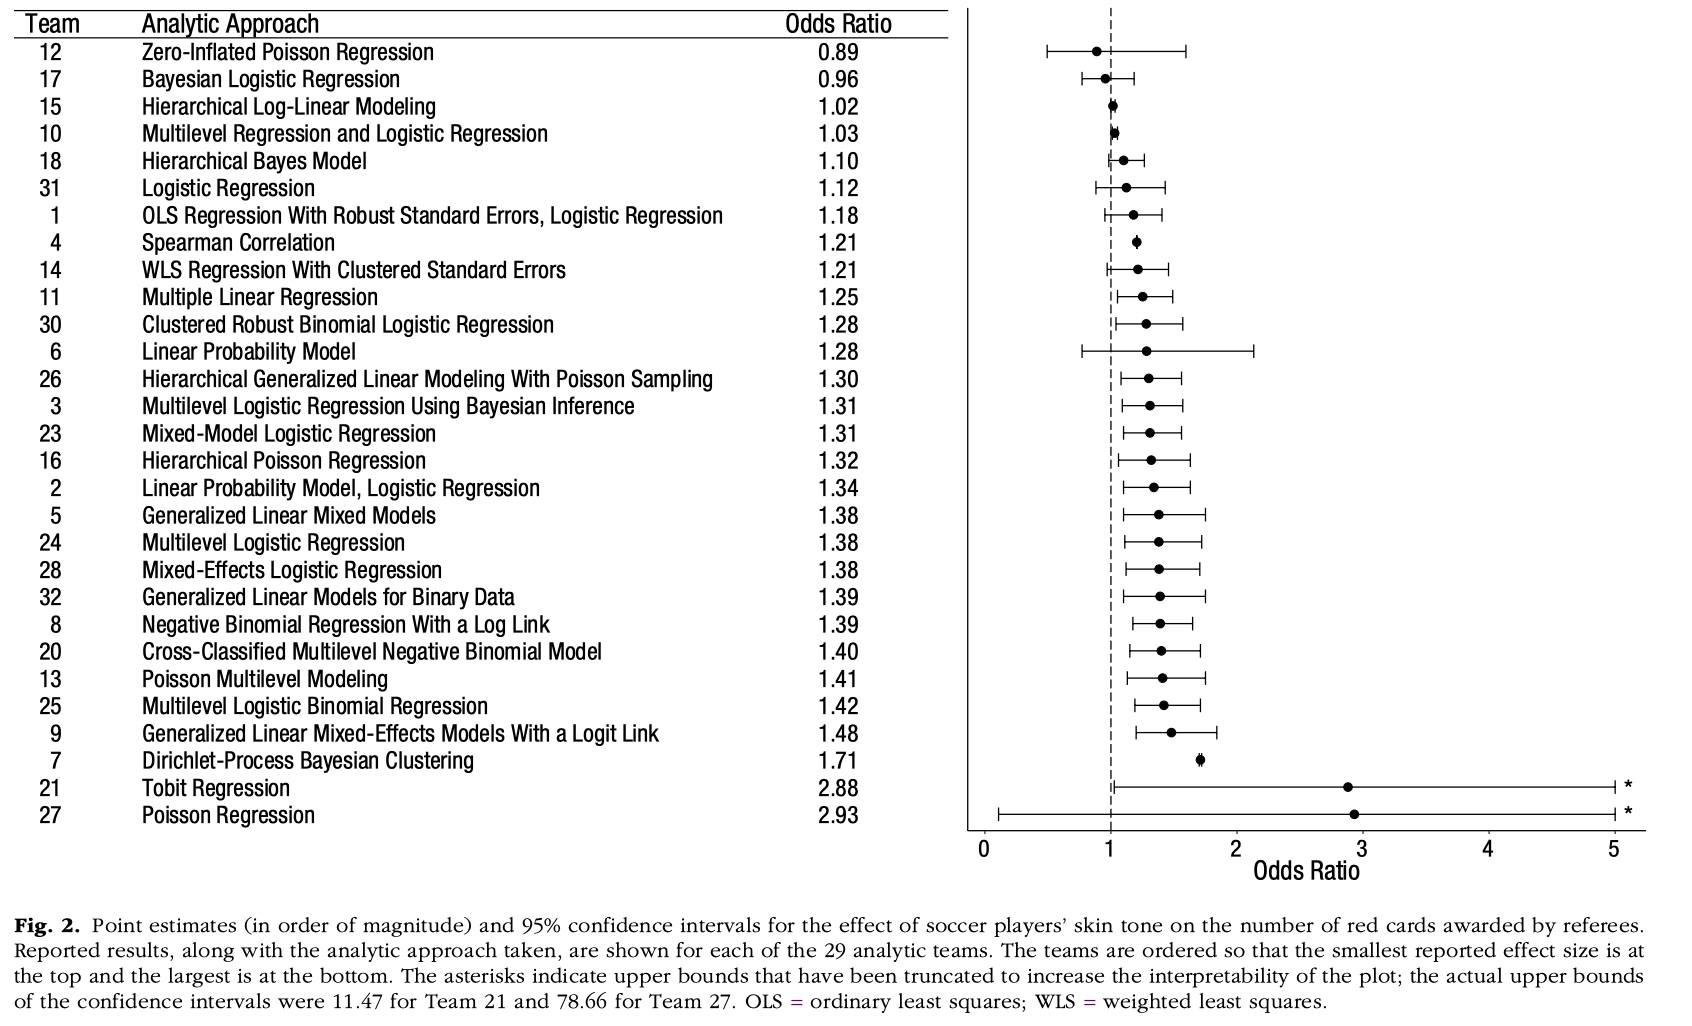
\includegraphics[width=16.51cm,height=10.02cm]{./images/soccer.png}
	\caption{Results from the Silberzahn study on soccer referee bias demonstrating the value of robustness tests on statistical approaches}
	\label{soccer}
\end{figure}


\paragraph{Existing refactors in the literature}

A conference poster "Reproducible Analysis in Practice with FireCloud" by the Genome Analysis Toolkit (GATK) group at the Broad Institute outlined attempts to perform a refactor of an existing exome study while applying WDL-compliant workflows, Docker containers, and Jupyter notebooks. This was very much in the spirit of this dissertation proposal, but because the underlying study involved protected data, the Broad group was forced to generate synthetic variants to mimic the original data set. While an admirable task, reverse engineering these called and filtered variants may introduce some weakness, as a major component of exome studies involves dealing with the vagaries of variant and genotype calling. Synthetically generating noisy data to imitate real noisy data only to arrive at the same intermediates may fall short of true reproduction.

\subsubsection{Robustness}

Here we define the robustness of an analysis as its ability to maintain core findings while withstanding perturbations introduced by tool and parameter changes. This is converse to the understanding of tool or model robustness - being able to be applied to a wide variety of experimental designs without returning spurious or biased results. The robustness should reflect both the experimental design and the strength of the underlying theory. The former is commonly known as "test validity" or, more specifically, "construct validity" - the degree to which a test measures what it claims to be measuring. \cite{OLeary-Kelly1998-ll}. The latter may reflect generalizability or "external validity," more generally "experimental validity," or scientific truth.

\paragraph{Understanding the history of omics method development}

To understand what makes it possible to perform tests of robustness, aside from justifying the practice as an evaluation tool, it is first necessary to explain why there are often many competing similar software tools that perform roughly the same tasks in the sciences. 

\begin{itemize}
	\item Different conceptual models - models can be derived from a physical or biological concept. For instance, many differential expression tools assume that there is a floor and a limit to the number of transcripts a cell transcribes in a given time, and that should inform the normalization of libraries derived from biological replicates. Other models may not be informed of the underlying biology but will strive for the best possible fit.

	\item Different statistical models - tools developed using different mathematical or stat models of the underlying phenomena will exhibit different error profiles in the face of experimental noise. One semi-recent example is the adoption of the negative binomial model to more accurately portray between-sample read count distributions ("dispersions") of next-generation sequence expression data.

	\item Different experimental scenarios - tools developed to address a specific question are often adopted by other areas without formal vetting - for example, fusion detection in cancer being used to detect readthrough events \cite{Haas2019-rq}.

	\item Different test sets - tools are developed to model-specific data sets available to developers will be fitted to those sets. This is often the root of complaints about tool description papers, as opposed to formal benchmarking papers, as a tool fitted or optimized to a test set will appear superior to untuned "straw men" competitors \cite{Buchka2021-fa,Peters2018-av}.

	\item Improved computational resources have enabled the implementation of computational approaches that would have been previously impractical. Both the transcript aligner STAR and the de novo assembler Velvet were developed during a time when single-node random access memory became available at gigabyte scale.

	\item Improved software implementations - this can be driven by the influx of developers from computer science or other disciplines and may take the shape of more modular, tested, or faster implementations.

	\item Improved algorithmic performance - Algorithms derived from other areas of mathematics, such as Burrows-Wheeler algorithm for compression, have provided indisputable improvement to omics tools, allowing either greater performance or more sensitivity with equal performance.

	\item Improved bias management - tools may improve as more data is collected about scientific instruments and biases are understood. In microarrays, MAS5 normalization has been largely replaced by RMA \cite{Lim2007-jb} and its successors, which utilize cohort normalization.

	\item Utilization of machine learning or deep learning approaches

\end{itemize}
A recent publication text-mining over 1000 single-cell tool papers revealed many of the trends above, with trends toward data integration, greater performance, and specialization \cite{Zappia2021-op}.

\paragraph{Degrees of Freedom and Questionable Research Practices}

To vet robustness testing as an evaluation tool, we must define the possible outcomes. The main theory behind robustness is that results are prone to inflations due to "researcher degrees of freedom," \cite{Bakker2020-qr} The flexibility afforded by computational choices enables both intentional and unintentional biases in the form of questionable research practices (QRPs). The most common types of QRPs are p-hacking, in which analyses are manipulated to achieve significance, and hypothesizing after results are known, in which the hypothesis driving an experiment is developed to explain a set of results as a confirmation, rather than a priori. Certain analytical approaches may invite these problems. Gene set enrichment analysis (GSEA) or Gene Ontology enrichment, for instance, are especially prone to QRPs \cite{John2012-lb} \cite{Timmons2015-yg,Wijesooriya2021-jc} because they so often generate results that can be explained post-hoc.

\begin{figure}[h!]
	\centering
	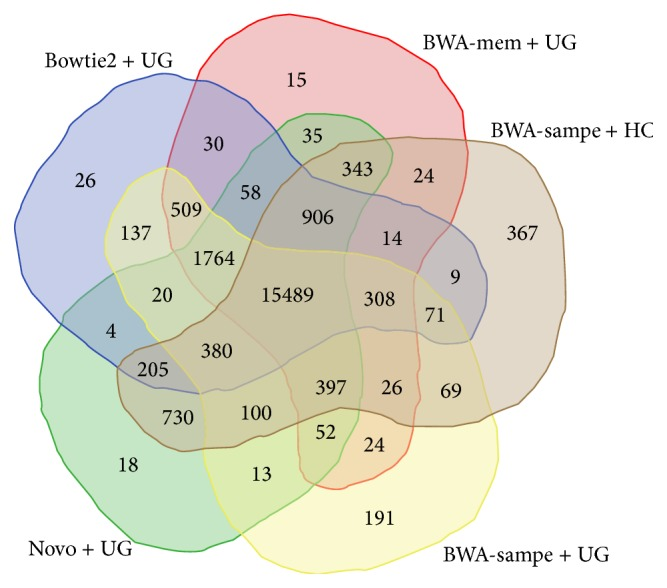
\includegraphics[width=13.76cm,height=12.09cm]{./images/venn.png}
	\caption{alignment-variant caller combinations}
	\medskip
	\small
	This Venn diagram from Cornish $\&$ Guda illustrates the lack of consensus among various alignment-variant caller combinations. In theory, each of these combinations could produce substantially different findings. \cite{Cornish2015-qo}
	\label{venn}
\end{figure}


\paragraph{Exploring Scenarios of Robustness Testing}

Though there is no formal determination for whether a test of robustness has "passed" or "failed", criteria should be developed from the results and discussions in the manuscript. The test of robustness may prove simply inconclusive if there are limitations such as lack of computing resources, software bugs, time, data accessibility that prevent it from being executed. Assuming a determination can be made by reviewers, multiple interpretations can be derived from that finding, and still, multiple conclusions and courses of action can be drawn from those interpretations.

\begin{itemize}
	\item Possible interpretations given analysis fails the test of robustness

\begin{itemize}
	\item The original tool or model is the "correct" model, and alternatives introduce error

	\item Authors engaged in one or more QRPs such as p-hacking, HARKing, multiple modeling

	\item Authors implementation contained software bugs

	\item Test of robustness itself contained software bugs

	\item The analysis is fundamentally flawed

	\item The effect is strong, but other tools in the robustness test are simply inappropriate, and only the analysis used will reveal the effect.

	\item The effect is weak, or detecting the scientific phenomena requires a particular set of tools and settings

\end{itemize}
	\item Possible interpretations given analysis passes the test of robustness

\begin{itemize}
	\item Test of robustness was too limited

	\item Both original tool and test models suffer from low test validity 

	\item Analysis is robust

\end{itemize}
\end{itemize}
Given the extensive time it takes to perform a test of robustness - a conservative estimate extrapolated from traditional peer review is 10 hours per reviewer and the experiences in this thesis suggests 20 to 100 hours may be more realistic - the peer review infrastructure should be revamped to yield downstream benefits from this work. An imagined endpoint that attempts to leverage yields from robustness testing is discussed further in the recommendations section.

\paragraph{Opportunities for robustness testing}

While a refactor is the most appropriate approach to test the state-of-the-art, the process of refactoring and modularization of steps should lend components of these analyses to be easily swapped out (i.e., a test of robustness). This task is a fortuitous opportunity as there is a renewed interest in systematic benchmarking of bioinformatic tools \cite{Mangul2019-cy} and statistical methods \cite{McIntyre2017-wr}, both of which greatly benefit from reproducible setups, especially modularized and parameterized workflows. Systematic robustness testing has not been conducted in any forum, but an extension of the REPLICats SCORE program \cite{Fraser2021-xc}, which reviews papers in eight social sciences fields, has proposed tests of robustness as an upcoming exercise. 


\begin{figure}[h!]
	\centering
	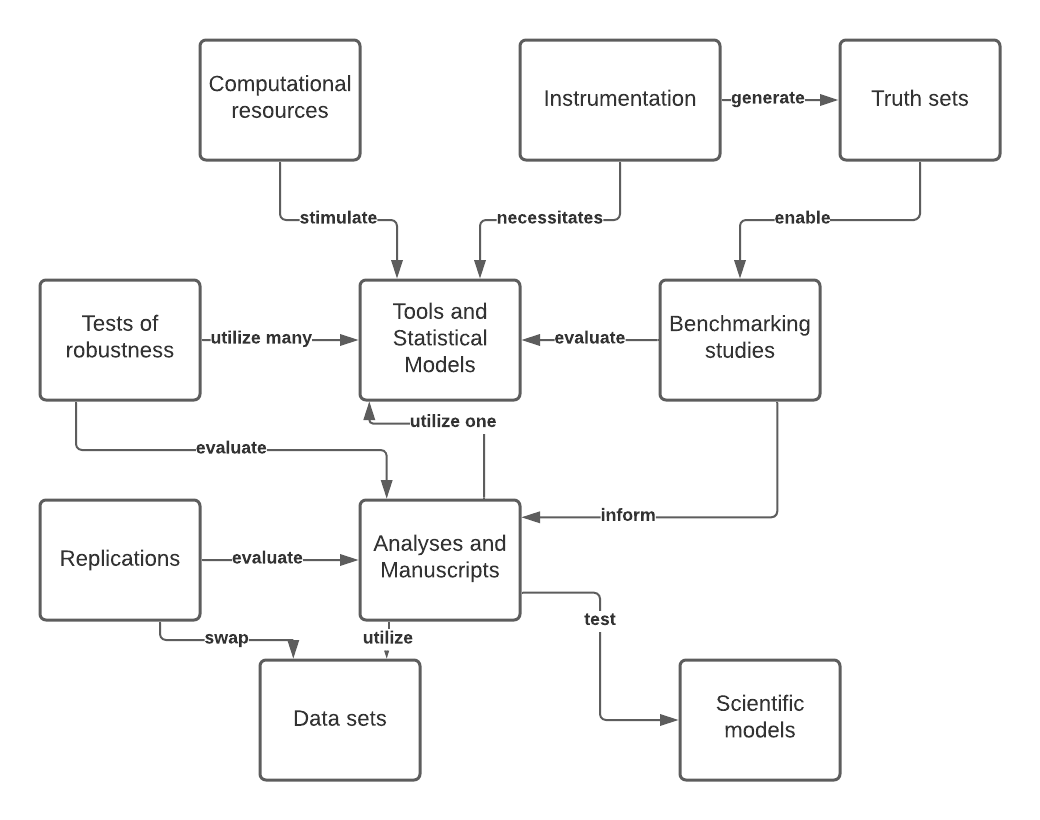
\includegraphics[width=13.76cm,height=10.81cm]{./images/concept.png}
	\caption{A high-level conceptual flow diagram illustrating the relationship between reproducibility-based evaluation concepts in scientific computing}
	\label{concept}
\end{figure}

\paragraph{Relationship between robustness testing and benchmarking}

A proper understanding of robustness testing requires disentangling its relationship of robustness testing, as benchmarking and robustness testing can be viewed opposite sides of the same coin. Robustness testing, as we define it here, involves evaluating an analysis under shifting tools, parameters, references, and data subsets. Benchmarking is an umbrella term for a variety of systematic tool measurements, but in this context, we can define benchmarking as testing tools or models against each other using defined gold standard truth sets or rubrics. In competitive machine learning circles such as Kaggle competitions, this gold standard would typically be a holdout test set sequestered from entrants. A well-known gold standard truth set in bioinformatics is Genome in a Bottle \cite{Zook2014-wy}, a collection of "High-confidence" variant calls and regions used in variant calling competitions. A benchmark without loss criteria or subjective judging is called a "bake-off" and typically involves groups with pipelines rather than individual tools. 

Disciplines that exhibit a high level of decision entropy and changing landscape of analytic tools, such as bioinformatics, are more likely to experience an extended vetting period in which both the tools and the analyses those tools are used in evidence for and against each other. As bioinformatics is one of the few disciplines where every paper draws scrutiny of both the underlying theory and the tools used to study it, every paper is an opportunity to engage simultaneously in benchmarking and robustness testing.

Tool papers are notorious for utilizing "straw-man comparison," unfairly favoring their own tool by overfitting to test datasets and leaving competitors often untuned or otherwise hobbled. Official benchmarking projects such as therefore, tend to take great care in establishing gold standard truth sets, typically triangulated through the intersection of several methods but also informed and refined by the tools themselves.

An interesting and novel part of this dissertation will involve a "user testing" component of robustness. Reviewers will be charged with swapping out a tool or statistical test from each analysis with an equivalent replacement and reporting the results.

Bioinformatic analyses lend themselves to tests of robustness because they often suggest several analysis choices of equal suitability. As discussed below, these analytical choices stem from different assumptions about the underlying biology, mathematical models at hand, computing power, and other criteria which change over a long period. An example of this phenomenon (one not used in this dissertation) is the decomposition or manifold learning of single-cell data. Single-cell studies study individual cells or clonal populations rather than bulk heterogeneous populations. A variety of genomic, transcriptomic (scRNA-Seq), and proteomic methods can be used to distinguish these populations. Most single-cell studies attempt to cluster and visually distinguish cell subtypes using dimensionality reduction (DR). The go-to technique for this since 2008 has been T-distributed Stochastic Neighbor Embedding (t-SNE) \cite{Van_der_Maaten2008-bm}. However, t-SNE has itself been criticized for low reproducibility in terms of achieving a given cluster for the same data, when adding new data to an existing set ("prospective stability"), or in preserving local or global cluster distances. A technique called UMAP reportedly produced more similar clusters using various subsamples of a data set than other tools, including t-SNE \cite{Becht2018-df}. As a first-order test of robustness, it would be desirable to implement UMAP on the raw data of a paper that uses t-SNE.

The above sections described existing case studies into reproducibility and presented robustness testing, in which tools, parameters, and data subsets are swapped out of existing analyses, as a natural extension of existing approaches that has been enabled by reproducible research and a practice that could be applied to peer review. These case studies informed the methods chosen for this dissertation. The next section presents my primary research questions guiding my work to implement robustness testing on existing published manuscripts with the intent to study both the requirements of packaging analyses for this exercise and evaluate the feasibility of this practice as a potential element of peer review.

\subsection{Goals and Objectives}

This dissertation addresses the primary question of whether reproducibility-enabled peer review, as implemented with tests of robustness designed to evaluate the strength of analyses, is feasible and practical given the state-of-the-art tools and standards. Secondly, this thesis is designed to reveal what is required for reviewers to conduct a test of robustness in terms of both software organization and computational environment. Finally, the dissertation seeks to identify the next steps to improve this process should it become standard practice.

The specific objects objectives of this dissertation are to 

\begin{itemize}
	\item Q1: Survey attitudes about reproducible research and tests of robustness from the participants, specifically feasibility and effectiveness. Do they differ from past surveys of reproducibility, notably Baker et al. \cite{Baker2016-ri} 

	\item Q2: What did the refactor process performed to prepare reviewers to perform subsequent tests of robustness, reveal about the underlying reproducibility and technical barriers to implementing these in practice?

	\item Q3: What did the tests of robustness reveal in the three papers?

	\item Q4: What are the pros and cons of the three approaches - faithful reproduction, workflow-library, and advisor-led - used during this study for tests of robustness?

	\item Q5: What gaps were identified in the process, and what solutions, metadata-based and otherwise, present themselves as next steps?

\end{itemize}
\subsection{Study Design}

\subsubsection{Methods}

This study employed a mixed-method methodology consisting of both user surveys and respondent-produced or respondent-directed analyses. A sample of three high-impact research papers was selected, each with open data and utilizing bioinformatic tools. These analyses, described only in the methods sections, were then refactored into pipeline frameworks to provide a basis for tests of robustness to be performed. Three different approaches were used. The first involved a complete reproduction of the paper for participants to manipulate, the second involved providing scaffolding for the use of pre-existing workflow libraries, and the third involved implementing expert suggestions in the form of tool swaps.

Three papers in genomics were selected based on criteria including data availability, significance, and critical reception. None of the papers featured open source code so refactors were based on descriptions in the methods section. Three different approaches were taken in these tests of robustness - a faithful reproduction of the original manuscript into a framework that could be manipulated by participants, a workflow-library approach in which participants were encouraged to employ modern "off-the-shelf" pre-built pipelines to triangulate tests, and an advisor-led approach in which senior experts suggested alternate tools to be implemented and I generated a report for their evaluation.

Participants were contacted about this opportunity via several means - through Twitter, Slack groups, message boards, and direct personal contacts. IRB approval was obtained before conducting the survey and test of robustness.

Figure \ref{studydesign} outlines the study design abstract. Three papers without source code, with often vague or high-level methods sections, were refactored - prepared for robustness testing by providing organized and reproducible source code that could be used to conduct robustness testing. The refactored code is available in Github. The refactoring process is meant to examine what is necessary for consumption by reviewers, in particular, what pain points are involved in preparing data for tool swaps.

\begin{figure}[h!]
	\centering
	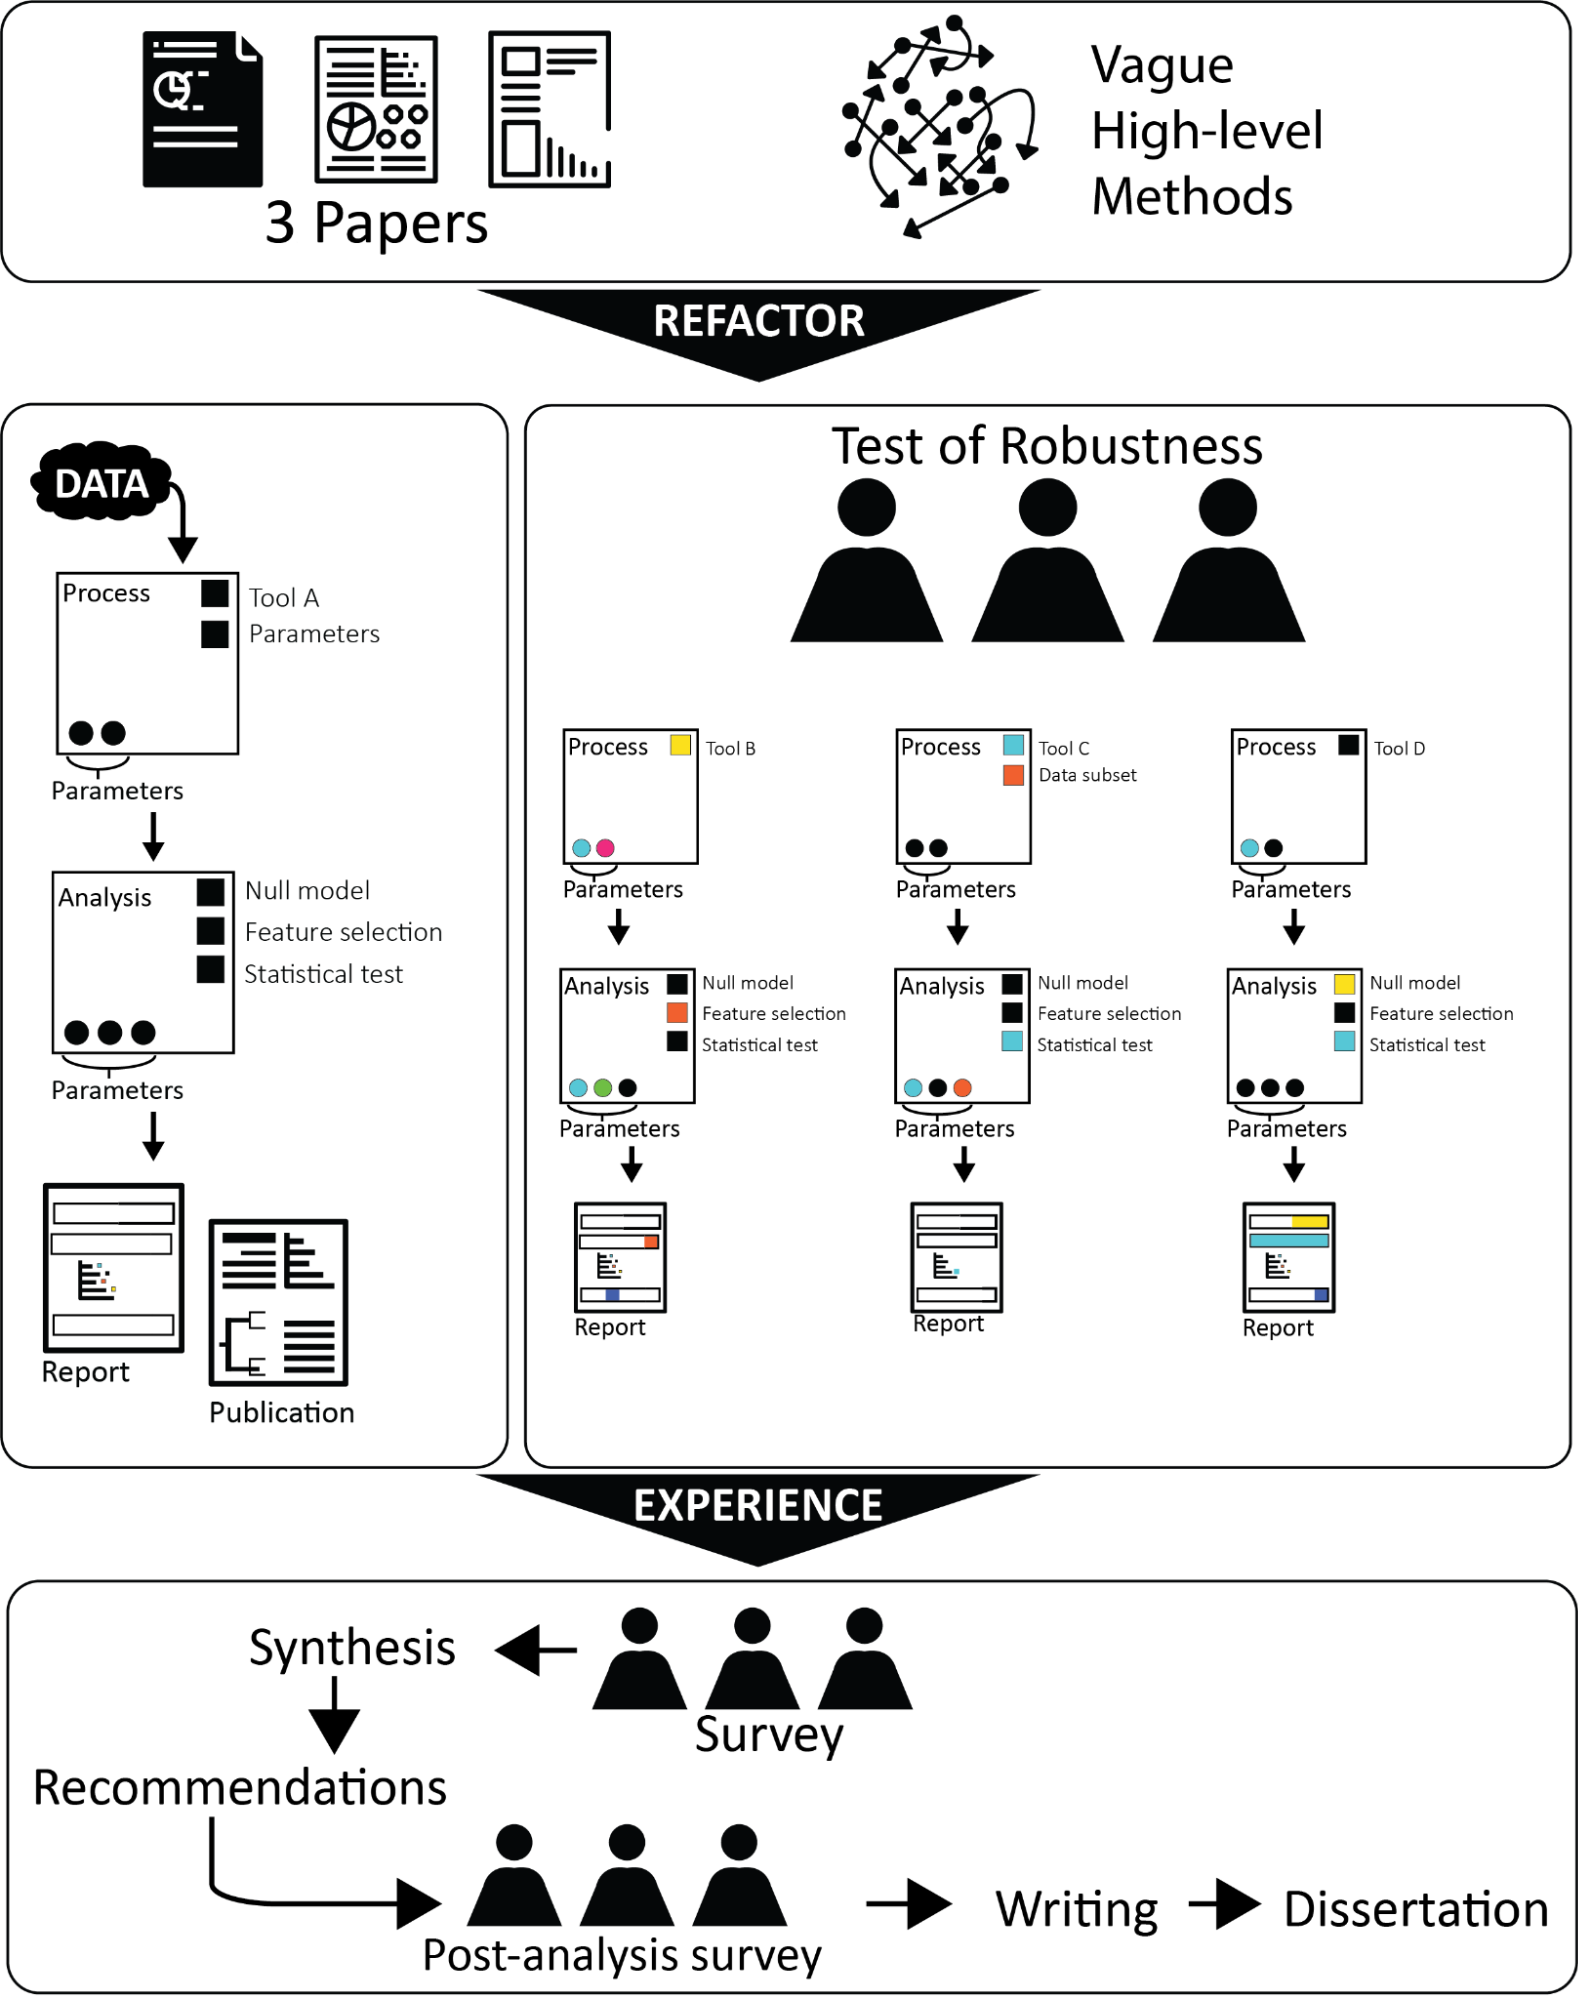
\includegraphics[width=13.76cm,height=17.36cm]{./images/studydesign.png}
	\caption{Study design diagram illustrating tests of robustness and evaluation phases}
	\label{studydesign}
\end{figure}



\subsubsection{Paper and environment selection}

\paragraph{Identifying Candidate Papers}

Candidate papers refer to studies that will undergo the tests of robustness. The candidate papers should be peer-reviewed life science research manuscripts, as opposed to software or tool papers. These should be recent publications (>$=$2010) with at least a nominal citation count (>$=$ 5 citations/year). Refactors in this scenario demand candidate papers that have a strong in-silico analytic focus, with substantial workflow and report components, as well as figures, tables, and test statistics to serve as targets. They must include open data (e.g., SRA or TCGA/GDC level 1, HMP) and either no open code or minimal refinement. Having no existing workflows are preferable in order to encourage full evaluation of the methods. Papers that feature highly parameter-sensitive approaches such as deep learning present some interesting possibilities, but the reproducibility challenges of deep learning are more complex than simpler approaches - being highly sensitive to random seeds and often the inclusion of non-deterministic steps.

\paragraph{Pipeline framework selection}

Pipeline frameworks provide means of abstracting file transformations common to bioinformatic analyses. Modern frameworks consist of domain-specific languages, which provide syntax used within full-featured programming languages, and configuration-based frameworks, which rely on formatted files with limited inline scripting to represent tools and steps of a workflow. There are four popular pipeline frameworks and languages used today - Snakemake, a DSL that relies on Python and uses a wildcard syntax to relate file inputs and outputs. Nextflow, a DSL in Groovy which uses abstracted channels to organize the flow of files through a pipeline rather than rely on filenames, Workflow Description Language, a JSON-based language developed at the Broad Institute that runs on an engine called Cromwell, and Common Workflow Language, a consortium-developed YAML-based language that runs on some graphical workbench portals in addition to command-line usage. CWL is the most verbose of these, but also offers the highest level of descriptive syntax for tools. It may be too verbose and heavyweight for rapid development and was therefore set aside for this exercise. WDL is very popular for genomic applications that rely on the Genome Analysis Toolkit (GATK), ENCODE pipelines, and other sequencing applications. Nextflow has a very strong community dedicated to building reusable pipelines, nf-core. Snakemake is popular among Python users and has a low barrier to entry. Because DSLs offer more flexibility in terms of rapid implementation and metadata management, they were used for the refactors. Snakemake was chosen for the Leiby paper as Sunbeam was already written in Snakemake. It was also used for Funnell et al. due to the amount of "business logic" involved in sample management, some of which overlapped with Leiby. Nextflow was chosen for the Dominissi paper to attract nf-core users and test the workflow library approach to robustness testing.

\paragraph{Computational environment}

If possible, a workflow portal to accommodate these analyses could be beneficial. To our knowledge, there are no free workflow portals - SevenBridges Genomic and DNANexus - are all for profit, but more importantly, not often used in institutions without close relationships to those companies.

Terra, a portal from the Broad Institute, uses the Workflow Description Language. The vast majority of public workflows in Terra are from the Broad Institute. A grant application to dispatch these reproductions on BioDataCatalyst - designed to encourage public workflows on such portals - was submitted but denied because the research was not novel.

All of the pipelines used in tests of robustness were suited toward running on Amazon web services or Google cloud platform. AWS offers a very convenient integrated development environment, Cloud9, which enables users to access an editor, terminal, and file browser from the web.

\subsubsection{Test of Robustness Approaches}

Three approaches were employed to conduct tests of robustness over the course of this dissertation. These approaches were not planned a priori but rather evolved from the experience of conducting the initial faithful reproduction - which resulted in conservative parameter sweeps instead of aggressive tool swaps. Interviews revealed this behavior was largely a matter of the intimidation factor involved in overhauling an existing workflow. The workflow library and advisor-led approaches were then implemented to ensure reviewers made more "aggressive" changes to assess robustness.

\paragraph{Faithful reproduction}

The faithful reproduction involves either interpreting a high-level methods section, as was done in this study or existing source code and refactoring it into available reproducible best practices for the benefit of the reviewers. These reviewers can then produce variations of the analysis as they choose to evaluate robustness.

\begin{figure}[h!]
	\centering
	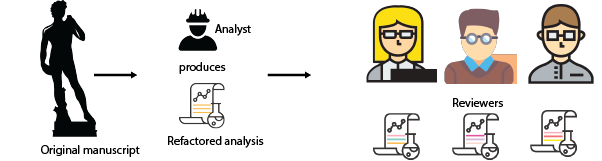
\includegraphics[width=13.76cm,height=3.66cm]{./images/faithful.png}
	\caption{Faithful reproduction approach}
	\label{faithful}
\end{figure}

\paragraph{Workflow Library approach}

The workflow library approach involves using off-the-shelf prepackaged workflows to process data from a manuscript. This ensures the analysis will be radically different from the original. Often these workflows offer variations in tools or parameters which can be explored for further refinement.


\begin{figure}[h!]
	\centering
	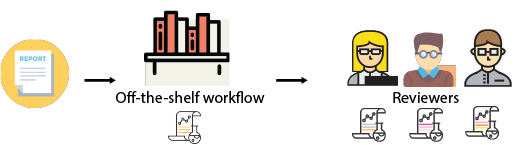
\includegraphics[width=13.68cm,height=3.84cm]{./images/workflow.png}
	\caption{Workflow library approach}
	\label{workflow}
\end{figure}


\paragraph{Advisor-led approach}

The advisor-led approach involves relying on the expert guidance of field experts to suggest tests of robustness, which are then implemented by an analyst. The results are sent back to the experts for interpretation.

\begin{figure}[h!]
	\centering
	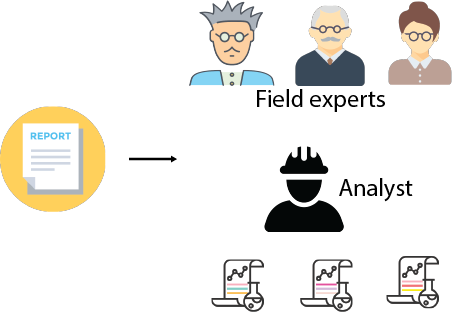
\includegraphics[width=13.68cm]{./images/advisor.png}
	\caption{Advisor-led approach}
	\label{advisor}
\end{figure}

\subsubsection{Selected Papers}

The following papers were selected for the refactors and tests of robustness based on various qualities they brought to the table. Leiby et al's "Lack of detection of a human placenta microbiome in samples from preterm and term deliveries" introduces a high decision-entropy area c16s and metagenomics) combined with a clear but important result of interest - that of the sterile placenta. Dominissini's "Topology of the human and mouse m6A RNA methylomes revealed by m6A-seq" was chosen because of its highly disputed citation record. Finally, Funnell et al. "CLK-dependent exon recognition and conjoined gene formation revealed with a novel small molecule inhibitor" was chosen because it targeted an area that has been traditionally underserved by toolsets (read-through splicing events) and utilized two types of sequencing.

\begin{table}[H]
\begin{adjustbox}{max width=\textwidth}
\begin{tabular}{p{2.75cm}p{2.75cm}p{2.06cm}p{3.44cm}p{2.75cm}p{2.75cm}p{2.75cm}p{2.75cm}p{2.06cm}p{3.44cm}p{2.75cm}p{2.75cm}}
\hline
\multicolumn{1}{|p{2.75cm}}{Paper} & 
\multicolumn{1}{|p{2.75cm}}{Topic} & 
\multicolumn{1}{|p{2.06cm}}{Citations} & 
\multicolumn{1}{|p{3.44cm}}{Reasons for Selection} & 
\multicolumn{1}{|p{2.75cm}}{Refactor Challenges} & 
\multicolumn{1}{|p{2.75cm}|}{Approach} \\ 
\hline
\multicolumn{1}{|p{2.75cm}}{Leiby et al. 2018} & 
\multicolumn{1}{|p{2.75cm}}{microbiome} & 
\multicolumn{1}{|p{2.06cm}}{152} & 
\multicolumn{1}{|p{3.44cm}}{High impact, workflow components, negative result} & 
\multicolumn{1}{|p{2.75cm}}{Tool decay, demanding reference generation} & 
\multicolumn{1}{|p{2.75cm}|}{Faithful reproduction} \\ 
\hline
\multicolumn{1}{|p{2.75cm}}{Dominissini et al \newline
2012} & 
\multicolumn{1}{|p{2.75cm}}{epigenomics} & 
\multicolumn{1}{|p{2.06cm}}{2384} & 
\multicolumn{1}{|p{3.44cm}}{Disputing citations} & 
\multicolumn{1}{|p{2.75cm}}{Arcane nf-core sample manifests} & 
\multicolumn{1}{|p{2.75cm}|}{Workflow-library} \\ 
\hline
\multicolumn{1}{|p{2.75cm}}{Funnell et al. 2017} & 
\multicolumn{1}{|p{2.75cm}}{splicing} & 
\multicolumn{1}{|p{2.06cm}}{30} & 
\multicolumn{1}{|p{3.44cm}}{Rare phenomena, dual-mode sequencing} & 
\multicolumn{1}{|p{2.75cm}}{Complex experimental design, deprecated sequencing formats} & 
\multicolumn{1}{|p{2.75cm}|}{Advisor-led} \\ 
\hline
\end{tabular}
\end{adjustbox}
\caption{Selected papers for tests of robustness}
\end{table}
\paragraph{Leiby et al}

Leiby et al. \cite{Leiby2018-lf} employs a multi-modal approach to studying a long-standing question of whether the human placenta inherits a maternal colony of bacteria (microbiome) or is sterile. Conditions include vaginal and Caesarean section delivery, preterm or full-term birth. Positive controls were taken from the mother's saliva.

16S rRNA qPCR'ed samples were sequenced on the Illumina MiSeq platform. 16S represents a small section of the ribosomal RNA that evolves at an appropriate rate to compare bacterial species and is a standard and well-established method of microbiome diversity studies. The majority of this analysis is done in Dada2 \cite{Callahan2015-eu}, and Qiime1 \cite{Caporaso2010-rh}.

A shotgun metagenomic analysis was performed on the samples as well. This amplifies genes from all cells in a sample, including background host tissue. Metagenomic analysis is arguably a more rapidly changing area of microbial bioinformatics. The majority of the metagenomic analysis was performed with Kraken \cite{Wood2014-zm}.

The findings in this paper, while addressing an issue having important implications for health. Unlike the majority of scientific papers, this manuscript features a "negative result" as its primary finding. This negative result has some implications for the role reproductions and tests of robustness can play in a review - typically, an author will be hypothesizing for specific microbial composition changes while here, the authors are simply claiming a sterile placenta. Though no replications have been performed, subsequent studies \cite{De_Goffau2019-zm} have primarily confirmed the findings in this paper, 

\newpage

\begin{figure}[h!]
	\centering
	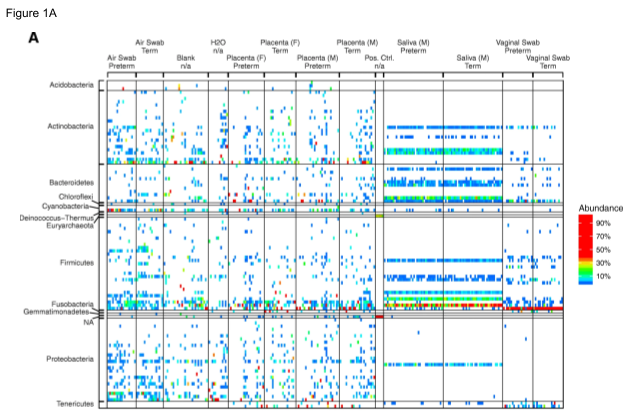
\includegraphics[width=\textwidth]{./images/leibyorig.png}
	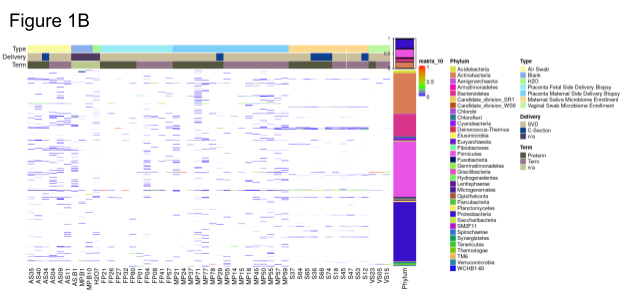
\includegraphics[width=\textwidth]{./images/leibyrepro.png}
	\caption{Original and reproduced bacterial abundance plots}
	\label{leibybac}
\end{figure}

\newpage

\begin{figure}[h!]
	\centering
	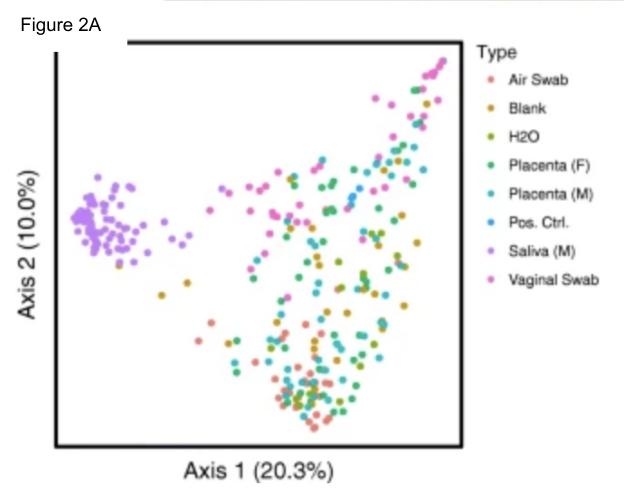
\includegraphics[width=\textwidth]{./images/pcaorig.png}
	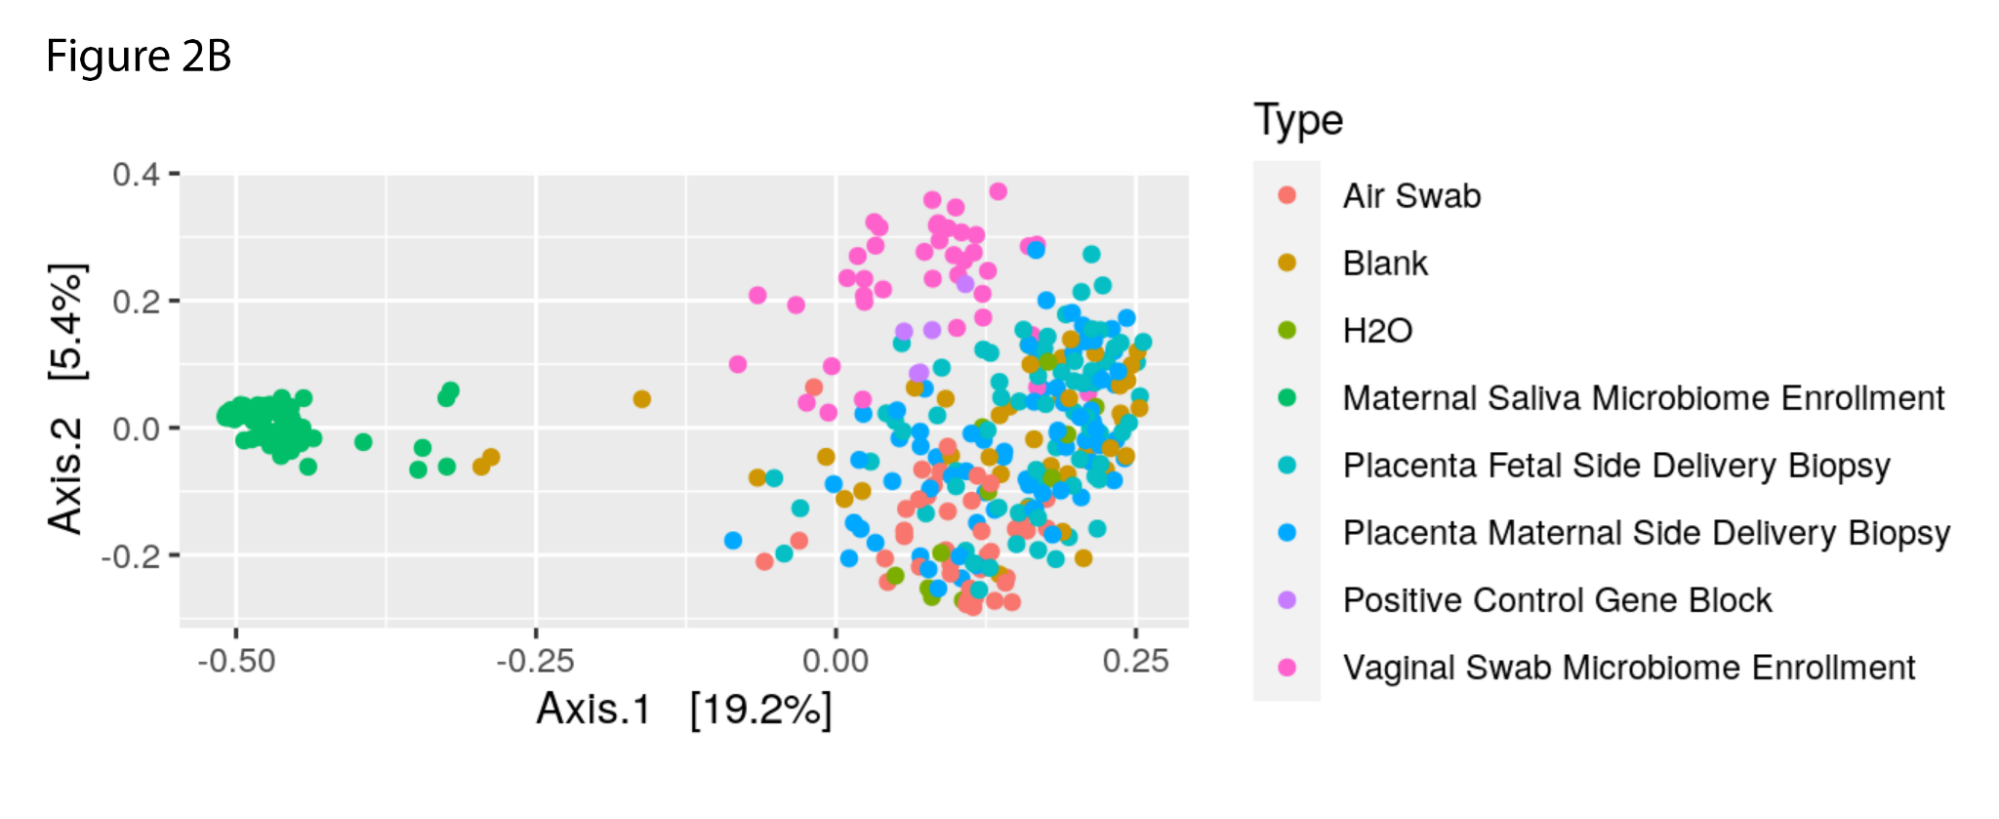
\includegraphics[width=\textwidth]{./images/pcarepro.png}
	\caption{Original and reproduced PCoA of unweighted UniFrac distances for all samples}
	\label{leibypca}
\end{figure}

As evidenced in Figures \ref{leibybac}A, \ref{leibybac}B and \ref{leibypca}A, and \ref{leibypca}B, the reproduction is not identical to the original and warrants further investigation. As described below, missing details in the methods section may have contributed to these discrepancies.

\paragraph{Issues in the Leiby refactor}

To review verbiage, we consider a reproduction to essentially mean a third party repeats an analysis with readily available source code. A refactor implies either the source code is missing or it is substantially replaced and reconfigured to high reproducibility standards. As mentioned in the proposal, papers were chosen based on having little to no source code. This was explicitly decided to force the refactor to closely examine the challenge of confronting decision entropy presented by inadequate methods sections. While the refactor involves a lot more reverse engineering and guesswork, it eliminates the possibility of glossing over impenetrable sections of source code, which may behave unpredictably. It can also detect insidious errors that arise from various common bugs such as:

\begin{itemize}
	\item assumptions of column or row order (typical slicing bug in R)

	\item Assumptions of mistaking index ordinal for cell value

	\item Assumptions in calling for indices instead of cell value (Python)

	\item cell shifts (as happened in the Potti scandal)

\end{itemize}
Leiby et al. presents typical challenges in terms of reproducing a paper with no source code and little in the way of supplemental in silico methods section. The tools and methods employed, while not exotic, still require a thorough reading of tutorials to reproduce these steps even before addressing more pressing issues of sample and parameter selection. Overall about 60 hours of labor were required to reproduce this paper. Dependency management and decay in the availability of dependencies, namely the dependence of python2 for Qiime1, required it to be isolated from other tools. Qiime1 also had numerous third-party dependencies that were deprecated or entirely missing (UCLUST implementation). Many scripts within Qiime1 attempt to fetch dependencies by unorthodox or non-standard means but are unable to find them, which required a system to preempt that processes within the Conda and pip dependency management systems. A significant amount of time was spent in what could be considered "data cleaning" tasks - mainly the alignment of naming schemes between SRA metadata schemes, files, and the sample metadata contained in the supplemental tables included with the paper. The refactor also required substantial effort to generate a multiple sequence alignment and tree building suitable to use with Phylotree within a reasonable time. Several tree building steps took on the order of hours and occupied nearly 100GB of RAM. Building the Kraken indices used by Sunbeam required over 8 hours of processing time and nearly 1TB of disk space. Vague methods obscured which operations were performed by potentially overlapping operations offered by Dada2, Qiime1, Phylotree, and RAXML. It would not be reasonable for a peer reviewer to engage in this level of reproduction for the sake of analysis, though such forensics have been done in the past on papers with no source code.

\paragraph{Causes of decision entropy}

The Leiby paper contains several "decision points" common to microbiome studies, some of which are omitted from the methods section. As with many studies, rationale explaining methodological decisions that stray from established best practices or default parameters are not provided. Other causes of entropy and ambiguity include:

\begin{itemize}
	\item Inadequate detail - which premade SILVA freeze and stringency (e.g. 97/99) was used

	\item Treatment of redundant sequence

	\item Treatment of chimeric sequences that can be placed in multiple clusters

	\item The effect of quality trimming \cite{Mohsen2019-er} on analyses in Qiime is significant.

	\item The unknown granularity of genus counts

	\item The cycle of threshold (Ct) qPCR data was not available to reproduce the figure 

	\item SILVA version was not given

	\item Operational Taxonomic Unit (OTU) compared to Amplicon sequence variant (ASV) approaches. The OTU approach uses a degree of sequence identity to form clusters. This prevents sequence data with small errors from being misclassified as novel species, although it can potentially cluster distinct species. Within OTU clustering are reference-free approaches, in which sequences are clustered de novo without a reference database, and reference-based clustering approaches which rely on prebuilt taxonomic databases such as SILVA, RDP, or Greengenes. Amplicon sequence variant (ASV) approaches such as the one implemented in Dada2 uses exact nucleotide patterns to distinguish marker sequences \cite{Callahan2015-eu}. In the Leiby paper, the early taxonomic assignments are handled by Dada2, but later measures of beta-diversity are calculated in Qiime using a reference-based OTU approach.

\end{itemize}
Dominissini/m6a

The second paper candidate for a test of robustness was selected based on its profile as a paper with a very high number of contrasting citations in scite.ai, an index that performs lexicographic full-text analysis on phrases flanking citations in scientific literature. In scite.ai, the vast majority of citations are neutral or "mentioning," some are "supportive," and a few are "contrasting." This assignment is performed solely by a machine-learning model based on the verbiage in those citing articles.

A highly-cited paper from 2010, Dominissini et al.'s "Topology of the human and mouse m6A RNA methylomes revealed by m6A-seq", received 13 "contrasting" citations in scite.ai, indicating some groups found different mRNA splicing in METTL3 knockdown cells, number of peaks, peak location, overall methylation levels. This paper is one of the first to develop a means of detecting a type of post-transcriptional modification, the methylation of adenine that has been implicated in expression and splicing and implicated in cancer and neurological diseases. While the wet lab advances in this paper were profound, the bioinformatic analysis was fairly conventional.

Post-publication reviews allowed the advantage of hindsight to identify a paper with glaring replication issues, which would not be available in a real-world situation. For a proof of concept, we can nonetheless examine if our approach could have identified such issues using robustness tests.

\paragraph{Workflow library approach}

The experience of the Leiby microbiome paper indicated most reviewers would tend to make fairly conservative changes to the pipeline rather than completely upend tools, the latter requiring more intimate knowledge of intermediate steps than could be afforded in limited time. An alternate approach was adopted to address this: rather than attempt to faithfully reproduce this paper using its original analysis stack, have used a couple of off-the-shelf pipelines to reanalyze this data.

The nf-core is a library of 50 Nextflow-based pipelines. These pipelines address a wide range of common analyses in bioinformatics including germline and somatic variant calling, RNA-Seq, ChIP-Seq, ATAC-Seq, to support several sequencing-based analyses. In particular, the workflows \url{https://github.com/eQTL-Catalogue/rnaseq} and \url{https://github.com/kingzhuky/meripseqpipe} were evaluated as appropriate. Reviewers could engage with the experimental layout using a custom generator that was developed to produce input manifests for these two pipelines. No reproduction code was provided to the reviewers to ensure they used nf-core modules and new tools.

\paragraph{Decisions in epitranscriptomic studies}

\subsubsection{Funnell/CLK}

Funnell et al.'s "CLK-dependent exon recognition and conjoined gene formation revealed with a novel small molecule inhibitor" (2017) investigates the effect of CDC-like kinase (CLK) inhibition. Alternative splicing is a fundamental biological process by which a multitude of mature messenger-RNA (mRNA) transcript isoforms are created from pre-mRNAs in eukaryotes. This occurs typically by splicing together (or skipping) exons or exon segments. Kinases are ubiquitous proteins that phosphorylate residues and are central to cell signaling. Because alternative splicing is mediated by RNA-binding proteins that interact with spliceosomes in the nucleus, kinases can affect both the quantity and variety of mRNA isoforms.

The authors of this paper created a novel molecule, T3, to inhibit CLK2, a known splicing-related kinase, to examine its effect on splicing patterns. They discovered that T3 produces more alternative splicing events, the skipped exons were enriched for RNA-binding motifs (DNA patterns that are used for recognition by RNA-binding proteins), and perhaps most interesting, a dose-response increase in conjoined genes (see below). Conjoined genes, or "transcription-induced chimeras" are the results of either readthrough events in which the RNA polymerase continues transcription into the next downstream gene or, less commonly, a distant gene.

This paper was selected because the bioinformatic tools to investigate differential splicing and isoform reconstruction are rapidly in flux and have changed considerably since its publication. Isoform detection and estimation took something of a back seat to simpler "percent-spliced-in" exon-centric differential splicing during the short-read era. Because genes are long (mean 3522 bp) and sequencing-by-synthesis (i.e., Illumina) reads are relatively short, transcript reconstruction must take an indirect approach of inference. This can involve de-novo assembly, which is computationally expensive.

Secondly, the group employed both short (Illumina MiSeq) and long read (Pacbio SMRT) sequencing, which further complicates the analysis, and leveraging these mixed reads is an ongoing area of research. Finally, the phenomenon of trans-splicing, read-through events where the transcripts of two genes are conjoined into single transcripts, is unusual and not a typically reported measure of transcriptome analysis tools. It remains a mystery how the conjoined genes in this analysis were detected using the MISO package as this is not a listed alternative splicing type in its documentation, nor are there other examples in the literature of using MISO in this manner \cite{Katz2010-ts}.


\begin{figure}[h!]
	\centering
	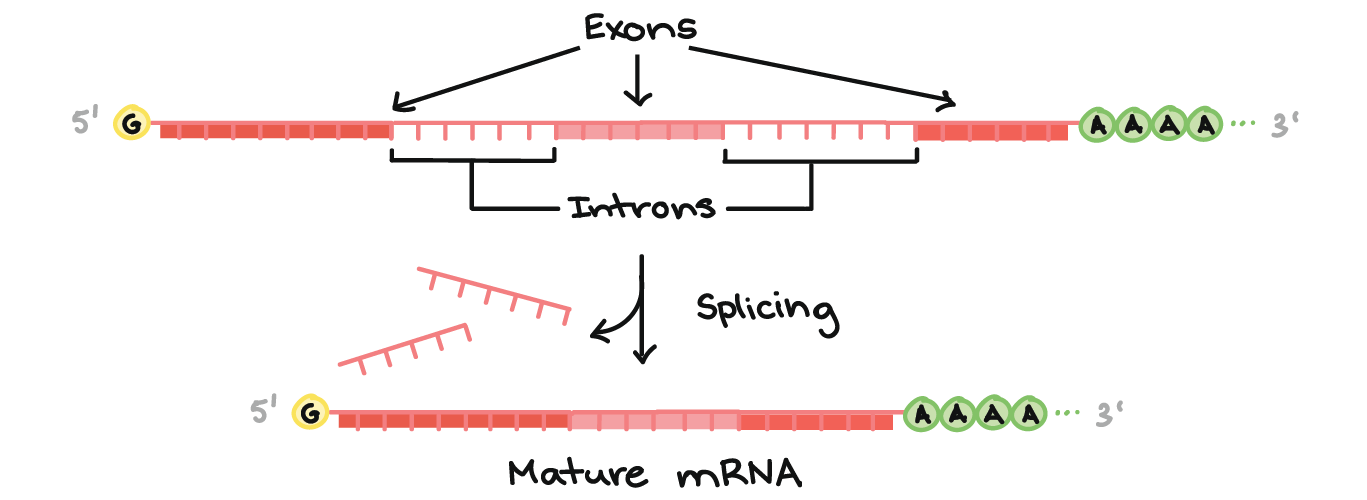
\includegraphics[width=16.51cm,height=6.03cm]{./images/splicemech.png}
	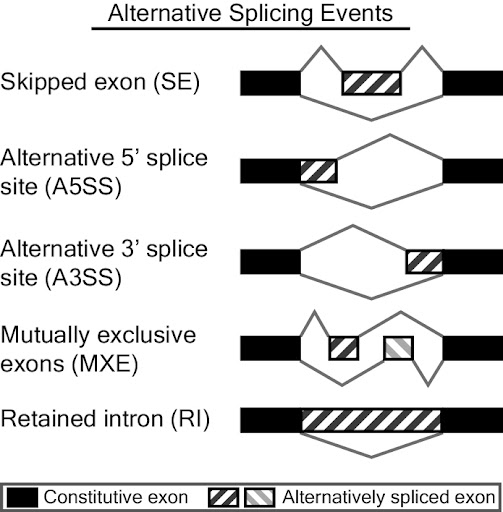
\includegraphics[width=13.31cm,height=13.55cm]{./images/splicetype.png}
	\caption{A) The mechanism of alternative splicing to produce different mRNA isoforms, and B) the different primary types of alternative splicing events}
	\label{splice}
\end{figure}

\paragraph{Approach: Advisor Model Tests-of-Robustness}

Due to the age of the manuscript and some of the tools within a direct reproduction of this paper was not attempted, but instead, three external advisors (YX, EL, were asked how they would investigate the phenomena described. I then implemented their suggestions and compared them to the results in the manuscript, a "naive" test of robustness. I term this proxy approach, in which a dedicated analyst performs the software development and implementation of the "advisor model," and its advantages and disadvantages to reviewer-implemented tests of robustness are discussed below.

\section{Results}

The results refer to results of the participant survey and critical first-order scientific observations drawn from performing tests of robustness rather than assessments of the exercise itself.

\subsection{Survey Results}

A survey questionnaire was distributed to each participant to collect views on reproducibility and specific gaps in reproducibility concerning reproducibility-enabled peer review. This survey was conducted simultaneously with the robustness exercise. Professional demographics and overall familiarity with reproducibility concepts, knowledge and usage level software, daily engagement with reproducibility best practices were surveyed. Several questions were used verbatim from Baker et al.'s "1,500 scientists lift the lid on reproducibility" and State of Open Data 2019\cite{Digital_Science2019-iu} to assess any drift in attitudes, and the results are mostly in line with those. While an N of 10 respondents is not an adequate sample size from which to draw firm conclusions, the survey can be viewed as a decent filter for the questions themselves (many questions exhibited low entropy). More interesting were ranking-style questions that forced a participant to prioritize.

One notable question lifted directly from Baker, ranking factors by how much they contribute to a failure to reproduce results. The top five reasons listed were lack of protocols, lack of raw data, selective reporting, insufficient oversight, and poor statistical power. This varies somewhat from the Baker results of selective reporting, pressure to publish, low statistical power, not replicated within the original lab.


\begin{figure}[h!]
	\centering
	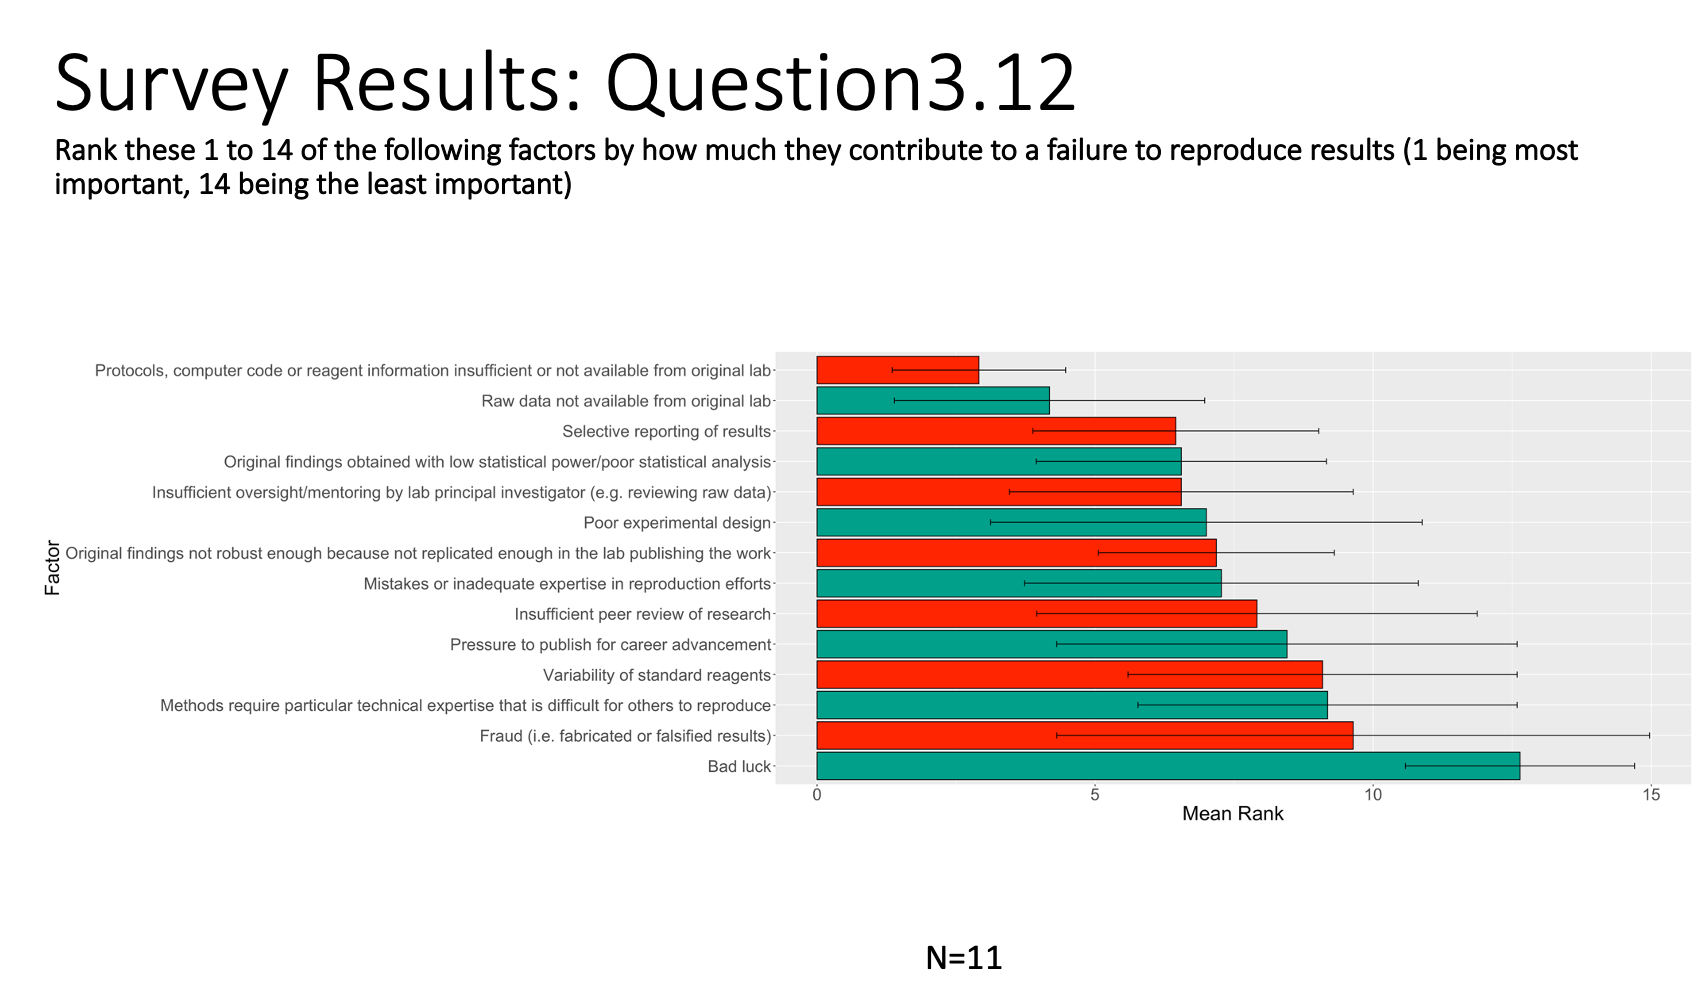
\includegraphics[width=13.76cm,height=8.08cm]{./images/surveyfactors.png}
	\caption{Survey of factors contributing to reproducibility failures}
	\label{surveyfactors}
\end{figure}

Some questions were designed to tease out a preference for replication vs robustness. Given replication is a far more well-known concept in reproducibility, it was assumed it would be more warmly received. However, votes were split evenly between them, with two favoring replicability, two robustness, and four stating these were equally important.

While 90$\%$ felt it was more (50$\%$) or equally (40$\%$) important that a scientific finding replicates with new data than with existing data. Six participants were unaware of preregistrations (Q8.3). Participants were also divided other where they would avoid journals that did not accept preprint (Q8.4)

Attitudes toward the open data, data sharing, need for increased recognition, difficulty in obtaining raw data from others, and the effect of missing methods (Q7.5), difficulty identifying paper figure provenance (Q7.8), and glossing of computational details (Q7.10) were strongly selected. Most agreed runnable analyses would be useful for peer review (Q9.2). Less pronounced were problems with label figures (Q7.6) and the role of sequencing providers(Q7.7).

In terms of ranking large categories of existing technologies as to how they contribute to reproducibility (Q6.2), all respondents identified dependency managers and containers, lightweight pipeline frameworks, and notebooks as contributing `` a lot" or ``a great deal," while workbenches, code commenting received slightly less enthusiasm.

Metadata played a role in some of the more important questions. Question 7.4 revealed that ``parameters used in an analysis" were viewed as most lacking, with raw omics, runtime environments, lab protocols tied, and bioinformatic tool metadata trailing. Q7.11 asked respondents to rank which metadata would help improve collaborative review most – metadata about raw data beat out tools and statistical tests, with metadata about other papers (by topic or method) judged less important.


\begin{figure}[h!]
	\centering
	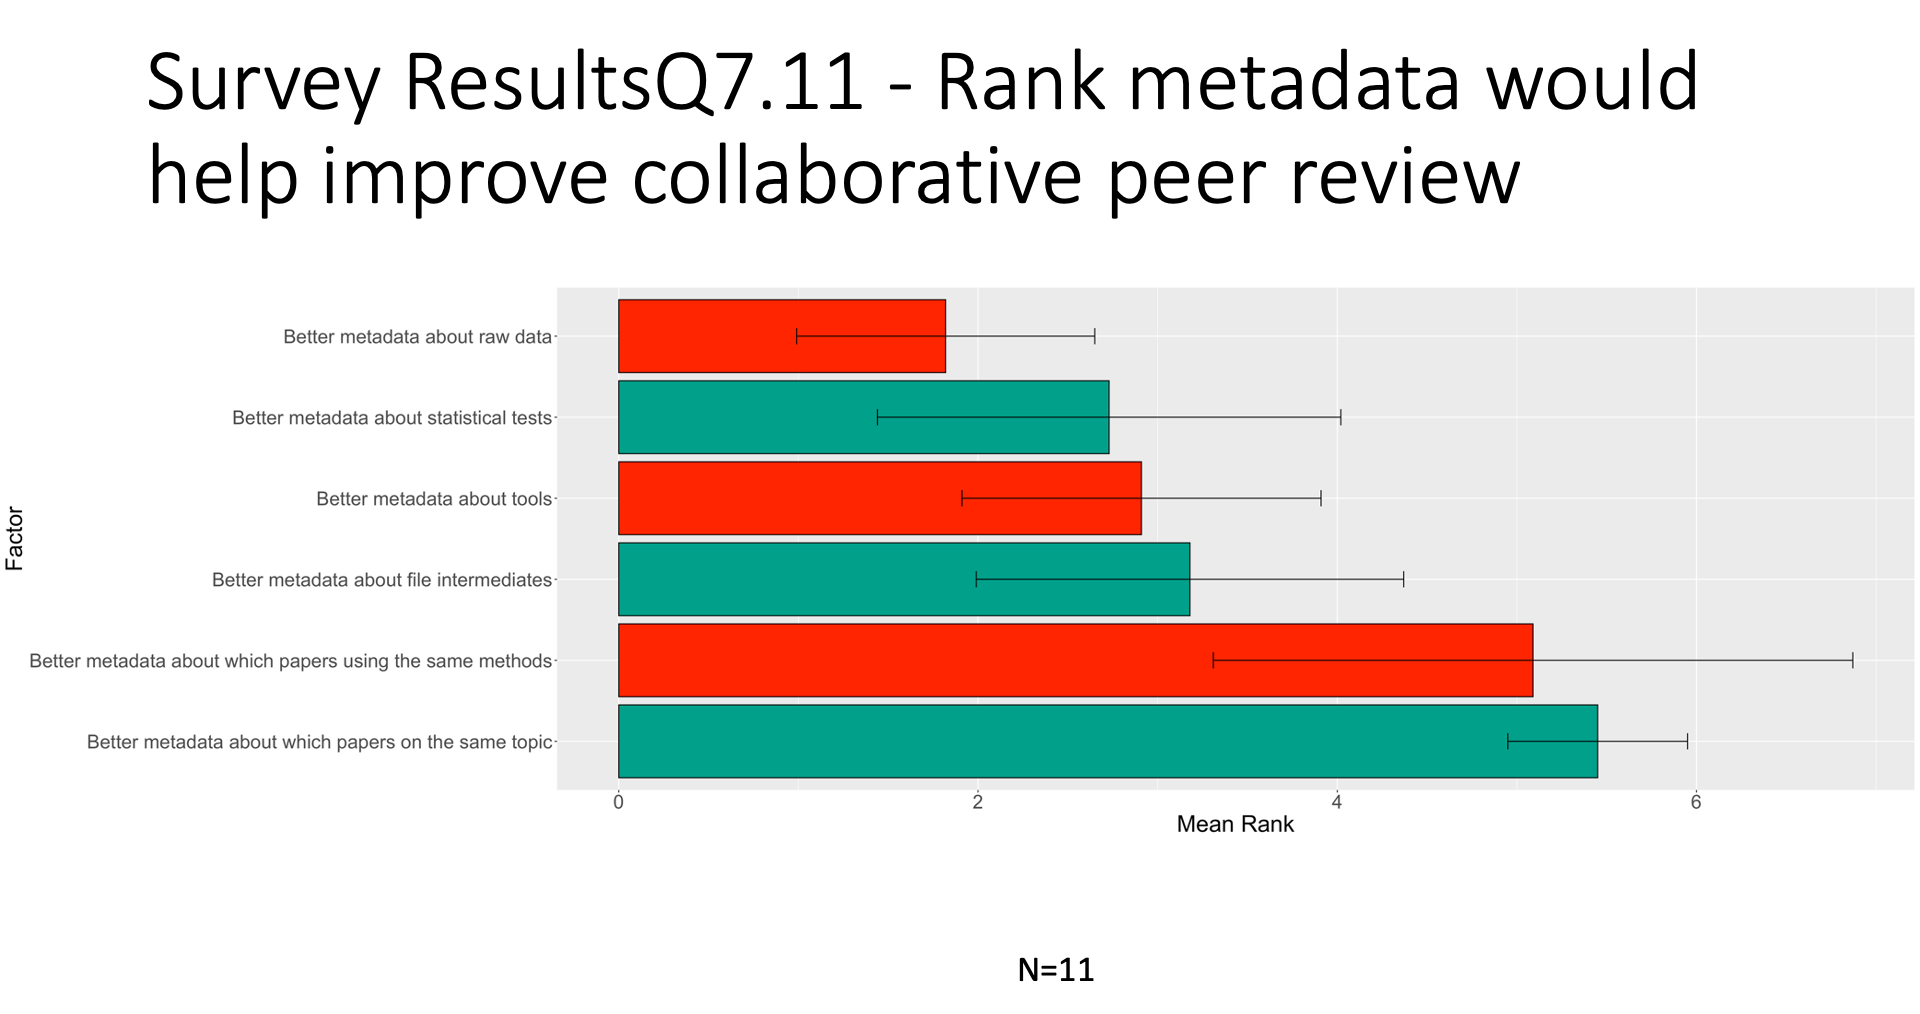
\includegraphics[width=13.76cm,height=7.23cm]{./images/surveymetadata.png}
	\caption{Survey of metadata to help improve collaboration}
	\label{surveymetadata}
\end{figure}

Perhaps the most divided question was ``do you find too much information about files is stored in filenames" (Q7.12), with four strongly agreeing and two either strongly or somewhat disagreeing.

See Appendix for Full Survey Results

\subsection{Robustness Testing Results}

The following section describes results of the robustness testing conducted by reviewers (in the faithful reproduction and workflow-library approaches) or by the analyst in the advisor-led approaches.

\subsubsection{Leiby/placenta}

\paragraph{Reviewer I}
Reviewer I is a tenure-track assistant professor with extensive experience in microbiome studies. During the entry interview, IB expressed confidence in the approach taken by Leiby et al. but less confidence over the rigor of microbiome papers in general.

Reviewer I conducted several permutations involving clustering algorithms, reference databases, and alterations of forward-only or forward-reverse alignments in UCLUST. The reviewer reported little substantial differences in Qiime beta diversity results from these permutations and provided Github code for those producing these permutations, though a readable report itself was not returned.


\begin{figure}[h!]
	\centering
	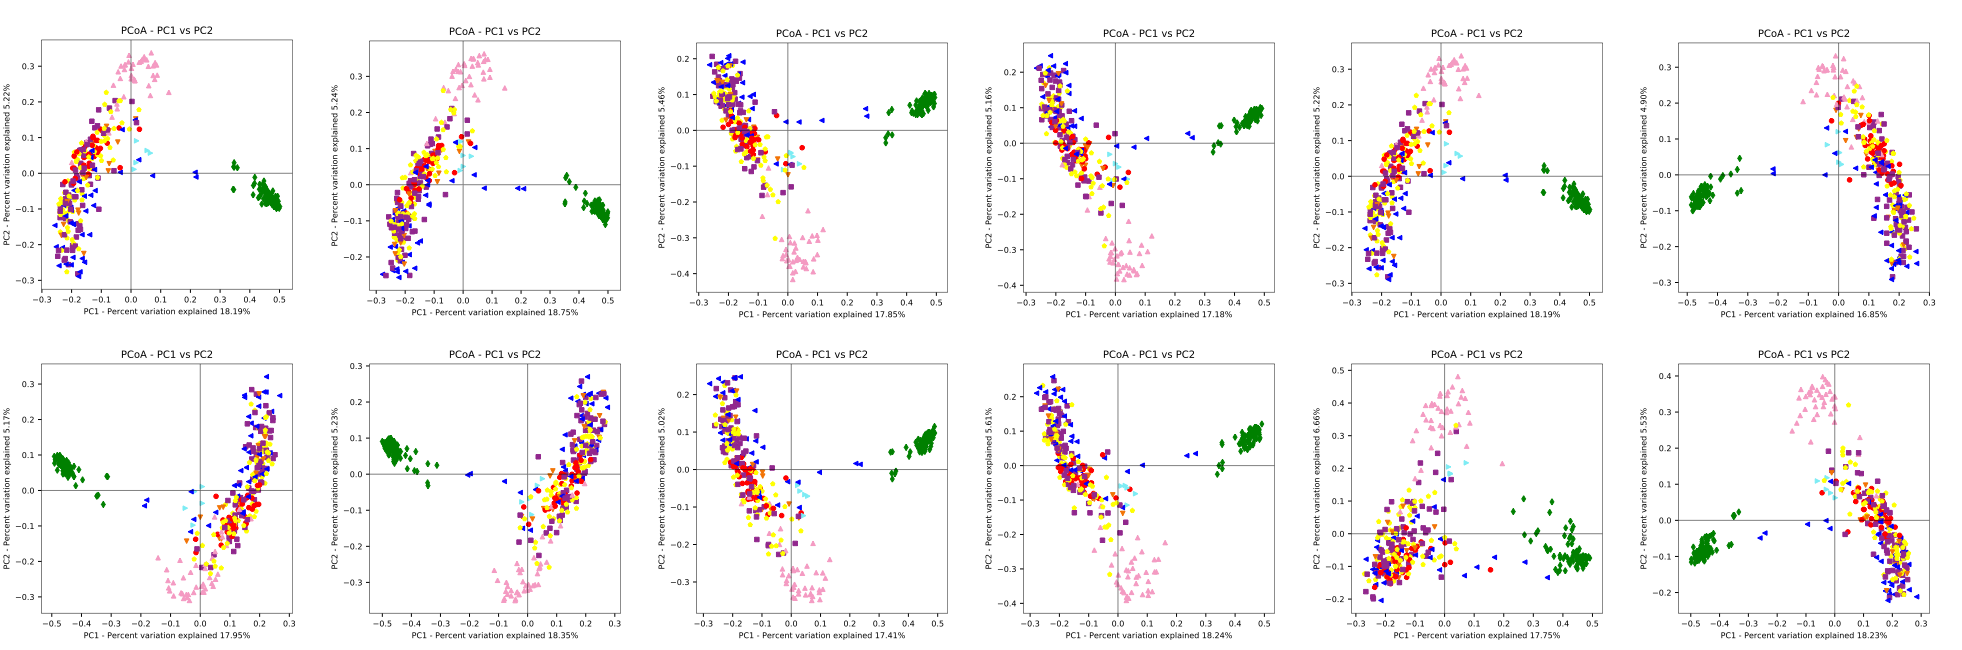
\includegraphics[width=\textwidth,height=5.47cm]{./images/betapermute.png}
	\caption{Reviewer I permutations revealed very similar beta diversity principal component analysis clusters}
	\label{betapermute}
\end{figure}

Reviewer I permutations revealed very similar beta diversity principal component analysis clusters

\paragraph{Reviewer II}

Reviewer II is a bioinformatics software engineer with authorship on several microbiome papers. Reviewer II performed several swaps of the "pooled" versus "consensus" chimera removal step in Dada2. Chimeras refer to artefactual sequences composed of two or more parent sources due to PCR amplification errors \cite{De_la_Cuesta-Zuluaga2016-fr}. Reviewer II performed iterations of terms of taxonomic assignment and sequence tabulation using the Ribosomal Database Project (RDP), Genome Taxonomy Database (GTDB), RefSeq, and SILVA 16S databases


\begin{figure}[h!]
	\centering
	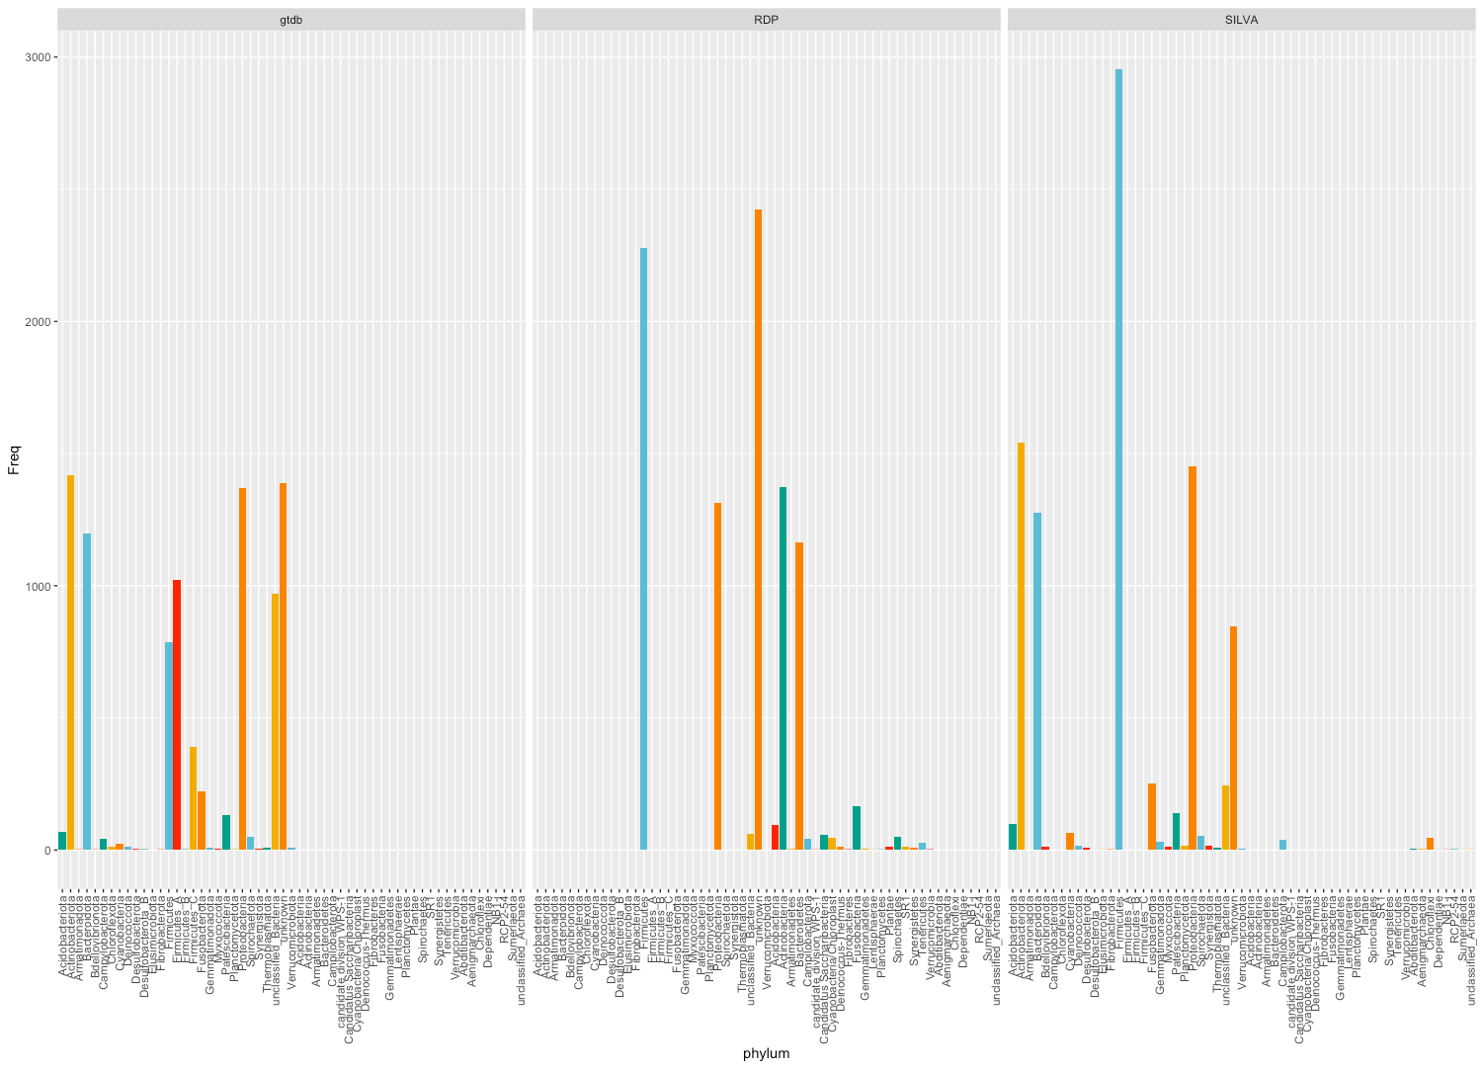
\includegraphics[width=\textwidth,height=11.89cm]{./images/decipher.png}
	\caption{Differences in phyla assigned by DECIPHER using three different 16S rRNA databases}
	\label{decipher}
\end{figure}


Reviewer II produced iterations of parameters sent to DECIPHER and dada2 - namely choice of 16s database, chimeric removal, and randomized taxonomic classifications performed by DECIPHER showing substantial differences in choices between gtdb, RDP, and SILVA 16s databases. Part of these differences can be discrepancies between naming conventions (Firmicutes vs Firmicutes A/B/C), and large differences in the assignment to the "unknown" phylum. The reviewer did not follow up to test if these assignments varied systematically between treatment groups.


\paragraph{Reviewer III}

The three participants were asked to collaborate on developing a high-level description of metadata that would have assisted in a first pass review of a microbiome manuscript. Reviewer III led this effort.

\subsubsection{Dominissini/m6a}

Dominissini et al. "Topology of the human and mouse m6A RNA methylomes revealed by m6A-seq" is a highly cited (>2000 citations on GS) paper that explores a type of RNA modification called N6-Methyladenosine or (m6A). Adenosine methylation is the most prevalent post-transcriptional modification in RNA \cite{Zhang2019-uh}, and has been identified as a core biological regulatory mechanism and dysregulation has been implicated in several diseases, particularly cancer and neurological disorders \cite{Jiang2021-kv}.

Dominissini et al. is one of the first to comprehensively map m6a sites using meRIP and also examined the effect of m6a methylation on transcription using a knockdown of a known acetylation complex component METTL3 using HepG2 cells, a human liver cancer cell line that is very common in splicing studies. Another experiment in this paper uses mouse cell lines. 

This particular paper was chosen for a test of robustness based on a methodical search using scite.ai, a text-mining and lexicographic tool designed to measure the context surrounding citations. Scite.ai uses deep learning models to classify citations as supporting, contradicting, or "contrasting," or merely neutral or "mentioning" \cite{Nicholson_undated-ry}. The vast majority of classifications in scite.ai are neutral. 

A scite.ai search revealed several papers that contained a high number of contrasting statements and also had accessible data in the NCBI Sequence Read Archive. A Twitter poll was conducted to gauge interest in these candidate papers, and Dominissini et al. was a clear favorite among the 14 respondents. Dominissini et al. has 175 supporting, 2600 mentioning, and 13 contrasting statements as of June 2021. The flanking text in all of the contrasting statements leaves little doubt that they are in fact, contrasting, which suggests there may be some false negatives in the neutral category (i.e. the classification algorithm is conservative).

Several contrasting statements are garnered from review articles that summarize later m6a publications which could be loosely considered replications. Because Dominissini et al. featured one of the first uses of m6A-seq aka MeRIPseq (methylated RNA immunoprecipitation sequencing) and associated peak calling, RNA-Seq, overlaps, in both human and mouse cells, there are downstream replications that are relevant. Contrasting statements included disputes about the level of mRNA splicing in METTL3 knockdown cells, number of peaks, peak location, and overall methylation levels.

The contrasting citations are important in that the instructions given to participants were instructed to use them as guidelines for further examination. This type of post-publication replication hindsight would not be available in a traditional peer-review model.

\paragraph{The workflow-library approach}

It was decided to accelerate the robustness exercise for this manuscript using "off-the-shelf" components, rather than modifying an attempt at a faithful reproduction. This was decided for three reasons. First, from the experiences with Leiby et al, as none of the participants were able to progress past the 16S section of the paper. This meant that the reproduction of the metagenomic components of the paper was done without proper robustness testing, though lessons were learned in the process. Secondly, the workflow-library approach offers some interesting advantages - such pipelines are well tested, reflect updated mainstream popular tools and approaches, have a large user base for support, often come with built-in reference sets, often have multiple implementation choices built-in, and are designed to work on several computing environments out of the box. Some disadvantages would make some papers inappropriate to be robustness tested in this manner - difficulty in customization, a lack of exotic or cutting edge protocols, and the need to conform to file manifests that may not match a specific experimental layout. However, these disadvantages did not seem to be insurmountable for this particular exercise. Finally, the age of this paper (11 years) made it somewhat impractical or desirable to reproduce faithfully.

Nf-core is a collection of prebuilt analysis workflows using the Nextflow pipeline framework \cite{Ewels2020-rf}. Over 47 pipelines are either released or under development in nf-core. Nf-core has a highly organized curation and testing process, with preliminary vetting guidelines for software development, including formatting, comments, and code organization. Finally, the nf-core community maintains an active Slack channel, making it easy to identify beginners or students who have the time and interest to participate in this exercise. To prepare participants to use nf-core for tests of robustness, manifest generators were developed for two pipelines identified as crucial - RNA-Seq, the most mature of pipelines in nf-core, and MeRIPseqPipe \cite{Bao2022-nk}, a new pipeline with applicable tools.

As identified in scite.ai, many later experiments failed to replicate some of the global changes identified in Dominissini. A review by Widalgo et al. \cite{Widagdo2018-vw} identified differences between the METTL knockdown experiments in mice conducted by Dominissi and two subsequent studies and a comprehensive and deeply sequenced gradation knockdown performed by Ke et al. \cite{Ke2017-lh} in mice. Some of these discrepancies may be due to species differences, some may be due to cell lines, but in no case were subsequent analyses harmonized to remove the analytic components as a confound. This result suggests that quantitatively little methylation or demethylation occurs in cytoplasmic mRNA. In addition, only 10\% of m6As in CA-RNA are within 50 nucleotides of 5\lq or 3\lq splice sites, and the vast majority of exons harboring m 6 A in wild-type mouse stem cells is spliced the same in cells lacking the major m 6 A methyltransferase Mettl3. It was noted that an open post-publication peer review site, PubPeer, identified the Dominnisi samples as being very contaminated with mycoplasma as identified by a survey of SRA \cite{Olarerin-George2015-hc}. This suggests a number of steps should be taken to avoid the deposition of contaminated samples pre-submission and begs the question of what role in silico peer review has in that process.

\paragraph{Issues in the Dominissini refactor}

The Dominissini refactor consisted of generating run manifests for the RNA-Seq and MeRIPseqPipe modules. Without the benefit of hindsight, it would have been very difficult to identify crux issues with this paper, being the first of its kind to use m6a-seq.

\paragraph{Reviewer I}

To examine the RNA-Seq data, one participant ran the RNA-Seq samples through the nf-core RNA-Seq pipeline. This reviewer discovered large descrepancies in the number of reported differentially expressed genes. Log-fold shrinkage is a feature of modern differential expression packages that reduces the apparent log-fold changes of genes or transcripts that appear to be artifactually inflated. Apeglm shrinkage applies a heavy-tailed Cauchy prior distribution for effect size, to lower variance for genes with low read counts or high variance \cite{Zhu2019-wo}. The use of log-fold change shrinkage became default behavior with DESeq2, but Dominissini et al. used the original DESeq, in which this shrinkage treatment was optional. In practice, this may have resulted in inflated DEG counts. After applying the filtering methods described in the supplemental methods, a more concordant count was found, though an overlap of only 59.8$\%$ was found between the original and refactored sets (Figure \ref{degenesinline}).

\begin{figure}[h!]
	\centering
	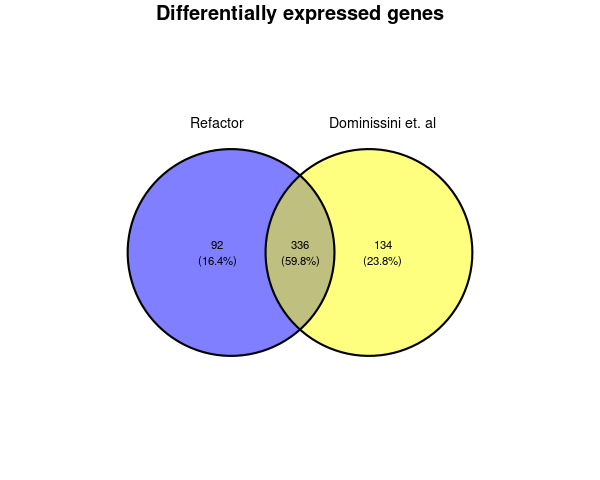
\includegraphics[width=13.76cm,height=11.05cm]{./images/degenes.png}
	\caption{Venn diagram of original and refactored differentially expressed genes in Dominissini et al. as discovered by reviewer I}
	\label{degenesinline}
\end{figure}


\paragraph{Reviewer II}

To examine the possible effect of workflow on the lack of replication by Ke et al, a participant was interested in performing a mini-replication within this exercise. This participant reported Ke et al. contained too much variety of paired-end and single-end reads to work easily with nf-core RNA-Seq, so the user switched to Xu et al. \cite{Xu2021-dx}, a mouse METTL3 knockdown. This allowed the comparison with the previously calculated human METTL3 knockdown data (the users were in contact through a Slack channel dedicated to this project within nf-core). It also allowed the study of the overlap of mouse m6a peaks reported in Dominissini et al. A permutation test showed the number of overlapping genes found between these two studies, one gene, was within random expectation.

\begin{figure}[h!]
	\centering
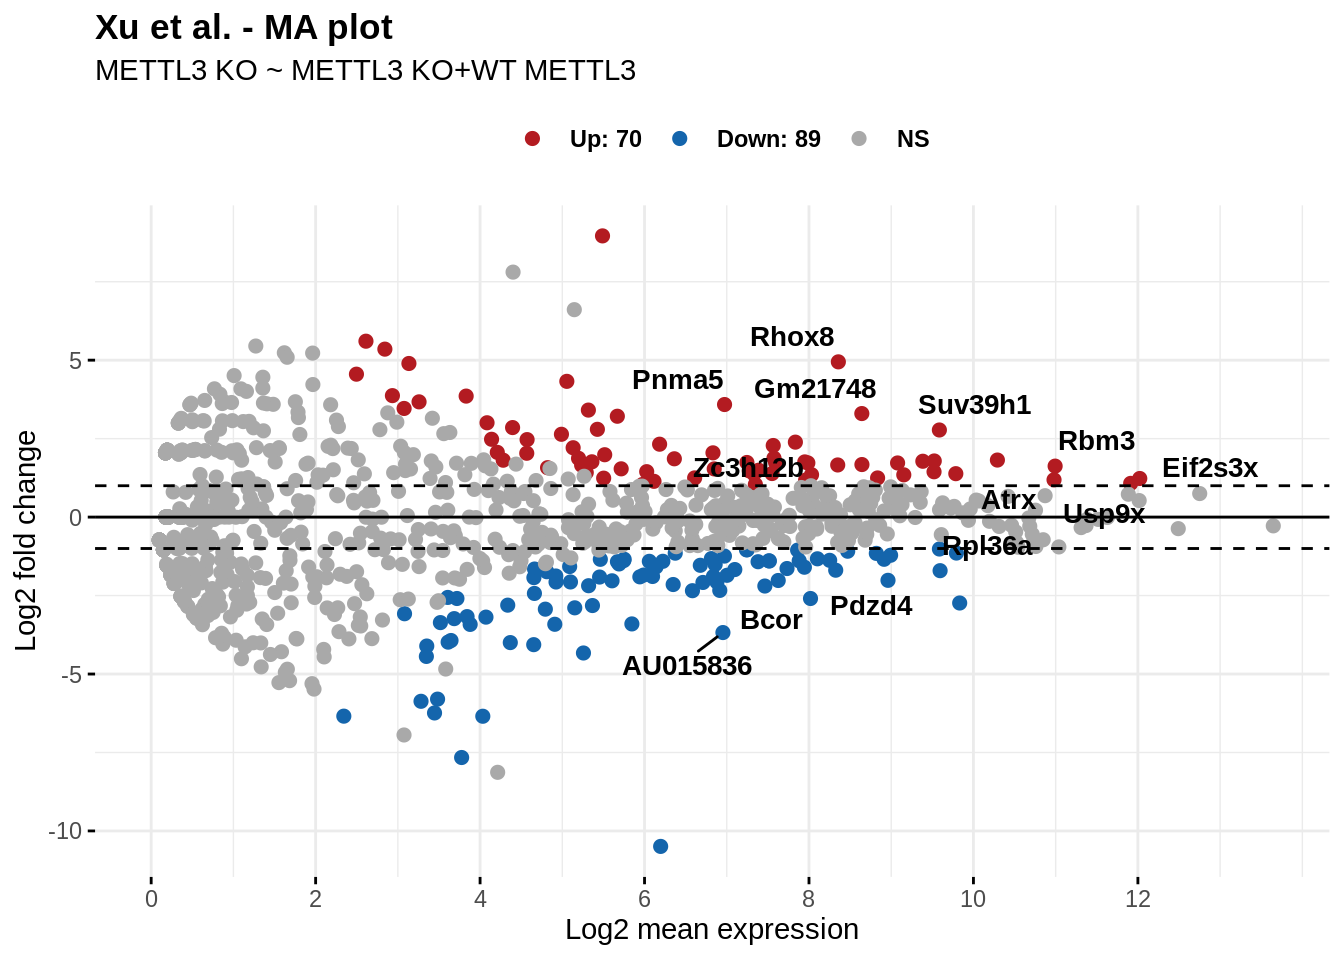
\includegraphics[width=13.76cm,height=9.78cm]{./images/ma6.png}
\caption{log fold-change versus log2 mean expression between two treatments in a Xu et al cite{Xu2021-dx} METTL3 knockdown in mouse.}
\end{figure}

\paragraph{Reviewer III}

Reviewer III attempted to use the MeRIPseqPipe framework to replicate the controversial figure 4. This pipeline is a candidate nf-core module, not yet vetted by the organization, and so created numerous issues in usage, some of which were later corrected in later versions of the pipeline that were released during the analysis. Some conventions - such as relying on gene\_type in gff files - made using older freezes impractical or highly inconvenient.

\subsubsection{Funnell/clk}

\paragraph{Issues in the Funnell refactor}

Funnell et al. consists of a mix of 170 Illumina and Pacbio libraries, with a variety of treatments (T3 at four doses, various siRNA knockdowns), human cancer cell lines (HCT116,184-hTert), and stranded/unstranded library preps. The panoply of sequence files required the development of a metadata management library ("metautils.py") to assist in generating both Snakemake targets and the appropriate input manifests for all the software requested by the expert advisors.

A WDL-based workflow based on the GTEX RNA-Seq pipeline located on a private workbench portal hosted at Truwl.com was used to accelerate the processing and take advantage of other QC outputs.

Various issues with the experimental metadata created difficulties in the refactor. The specification of which libraries are stranded/unstranded RNA is not located anywhere in the metadata except deeply embedded in sample names ("Untreated HCT116 whole transcriptome (unstranded)"). While not fatal, this added an additional step to the parser which would not be useful for other projects. A universal SRA manifest-generator would have to accommodate these types of edge cases. The use of older bas.h5 PacBio reads required an archived tool "bash5tools.py" which only worked with Python 2.7, which was deprecated at the end of 2020. This required a separate Conda environment.

Several installation and runtime issues were experienced with rMATS-Iso and SUPPA. While rMATS is production-level software used by hundreds of researchers, rMATS-Iso is still a beta distribution and was selected by one of the reviewers to evaluate its potential.

The lack of widespread user testing for rMATS-Iso led to some lack of a base from which to draw proper parameters for the older-style PacBio reads included with the Funnell paper.

\begin{figure}[h!]
	\centering
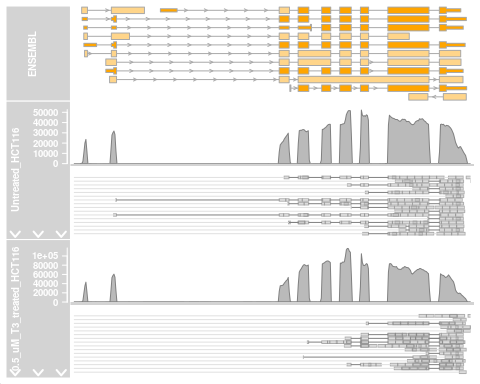
\includegraphics[width=12.83cm,height=10.27cm]{./images/asm.png}
\caption{Complex differential splicing patterns as revealed by rMATS-ISO}
\end{figure}

SUPPA utilizes pseudo-alignments generated against the transcriptome (typically in Salmon or Kallisto). As such the consistency between transcript FASTA files and gene models (GTF) must be preserved. One bug encountered was the additional transcript identifiers found in definition lines caused errors in SUPPA, which were not reported anywhere. Another cryptic bug appeared with low numbers of mapped reads, which forced the omission of certain replicate files provided as addendums.

The initial mapping qualities for Illumina reads using the default k-mer index of Salmon (31) were very low (<50$\%$). Upon closer inspection of the fastq files, many reads were shorter than 45bp, indicating some quality trimming was done prior to submission to SRA. This was not indicated in any SRA metadata. An index length of 17 was chosen to accommodate these shorter reads based on advice in help forums.

Very low mapping rates continued to appear for the PacBio reads. It was noted that "consensus generated" reads at EBI were mapping better than h5 extract fastq files. Upon closer inspection of the manuscript, there were suggestions that the PacBio reads, which constituted 60 of the 169 sequence files, were mainly used in an ad-hoc confirmatory basis. Finally, the inclusion of so many similar tools is that many auto-fetched roughly, but not identical, reference files. This required carefully harmonization of decoy sequences and other reference-specific anomalies to be rectified.

\begin{figure}[h!]
	\centering
	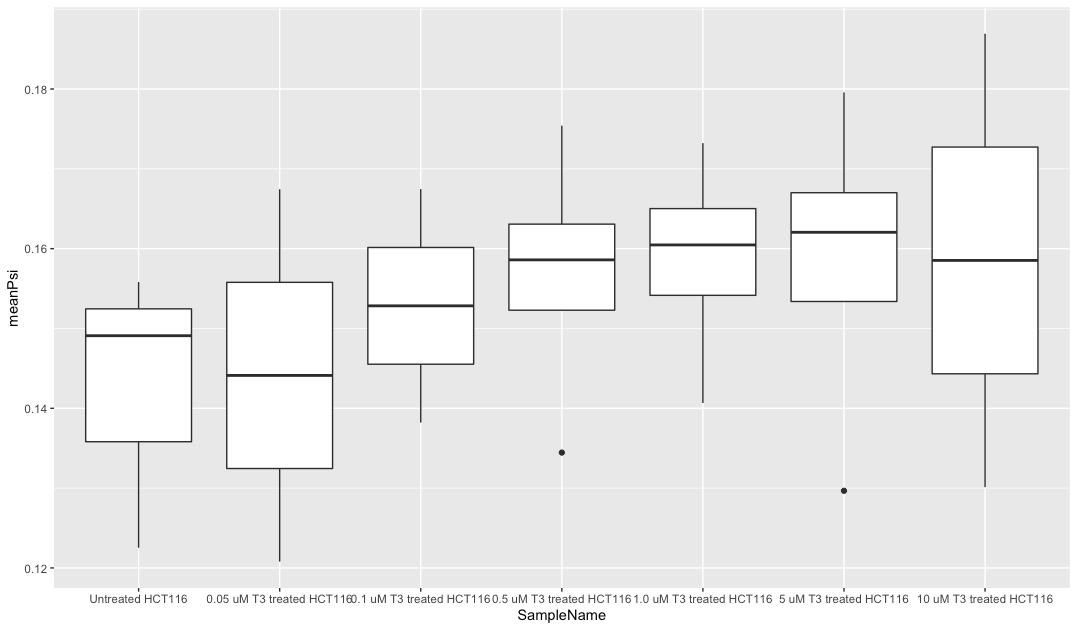
\includegraphics[width=13.76cm,height=8.03cm]{./images/arriba1.png}
    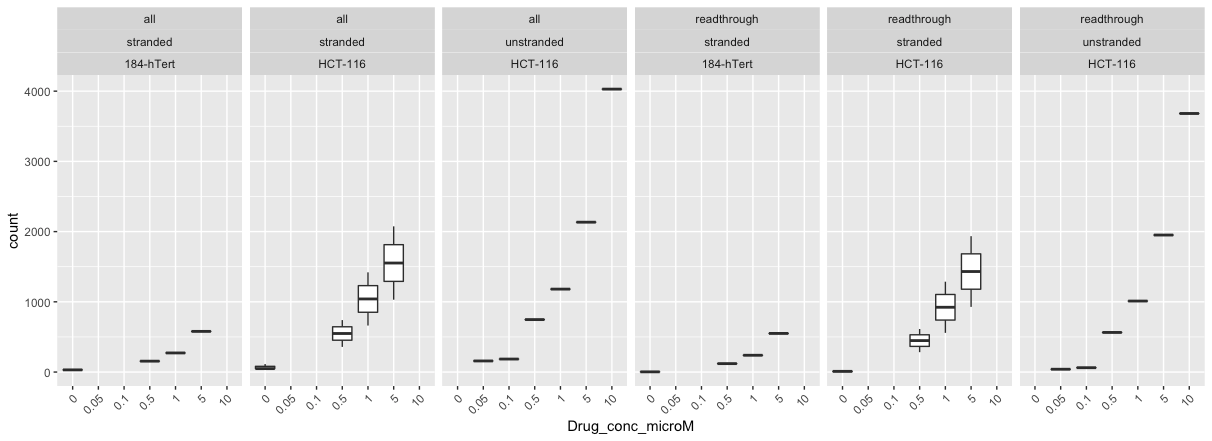
\includegraphics[width=13.76cm,height=4.98cm]{./images/arriba2.png}
	\caption{Percent spliced in (PSI) and counts of fusions by Arriba largely confirm the monotonic dose-response, with the vast majority of fusions being classified as readthrough events.}
	\label{arriba}
\end{figure}

Counts of fusions by Arriba largely confirm the monotonic dose-response, with the vast majority of fusions being classified as readthrough events.


\section{Discussion}

Research questions about the survey (Q1), refactor process (Q2), tests of robustness results (Q3), tests of robustness approaches (Q4) and gaps and next steps (Q5) were presented in the introduction.

\subsection{Q1: Survey responses}

The survey was largely in line with earlier surveys such as the landmark Baker et al. \cite{Baker2016-ri}, with more sentiments leaning toward nefarious intentions. More importantly, a general acceptance of the principle of robustness testing in peer review, and paid peer review, which has not been surveyed or studied in depth. 

\subsection{Q2: Refactor issues}

Before commencement the thought that the refactor issues would be centered around dependency management. These are largely resolved by bioconda, which provides dependencies for nearly all tools used in these analyses.

Participants were encouraged to accept a full Cloud9 IDE environment in the Amazon Web Services, which would provide the file browser, terminal, and code editor in one web application that can be accessed anywhere and retains state.

Notebooks do not yet play as big a role in bioinformatics as in data science, due to the large number of bulk operations that have typically been involved. However, knitr/RMarkdown reports were generated for all three analyses. As an exercise, two of these were ported to CodeOcean. They did not play a factor in the tests of robustness because most of the decision points were upstream, in the processing steps normally handled in the workflow rather than the notebook.

\subsection{Q3: Validating the Theory of Robustness Testing}

The theory of robustness testing presented here is not well vetted within the life sciences, and the term robustness itself is more likely to be used in the context of methods than analyses and is rarely discussed in the context of peer review. There is a precedent from other fields, namely multiverse analysis in psychology \cite{Steegen2016-zx} which is defined as alternatively processed data sets corresponding to a large set of reasonable scenarios. Note this is different from triangulation, which involves interrogating a scientific phenomenon using a multi-omics approach \cite{noauthor_undated-xz}. This dissertation attempts to measure the feasibility of this approach from a logistical standpoint rather than attempting to quantify the effectiveness of robustness testing in comparison to conventional peer review, as the latter seems largely dependent on the source papers.

\subsection{Q4: Comparison of Approaches}

\begin{figure}[h!]
	\centering
	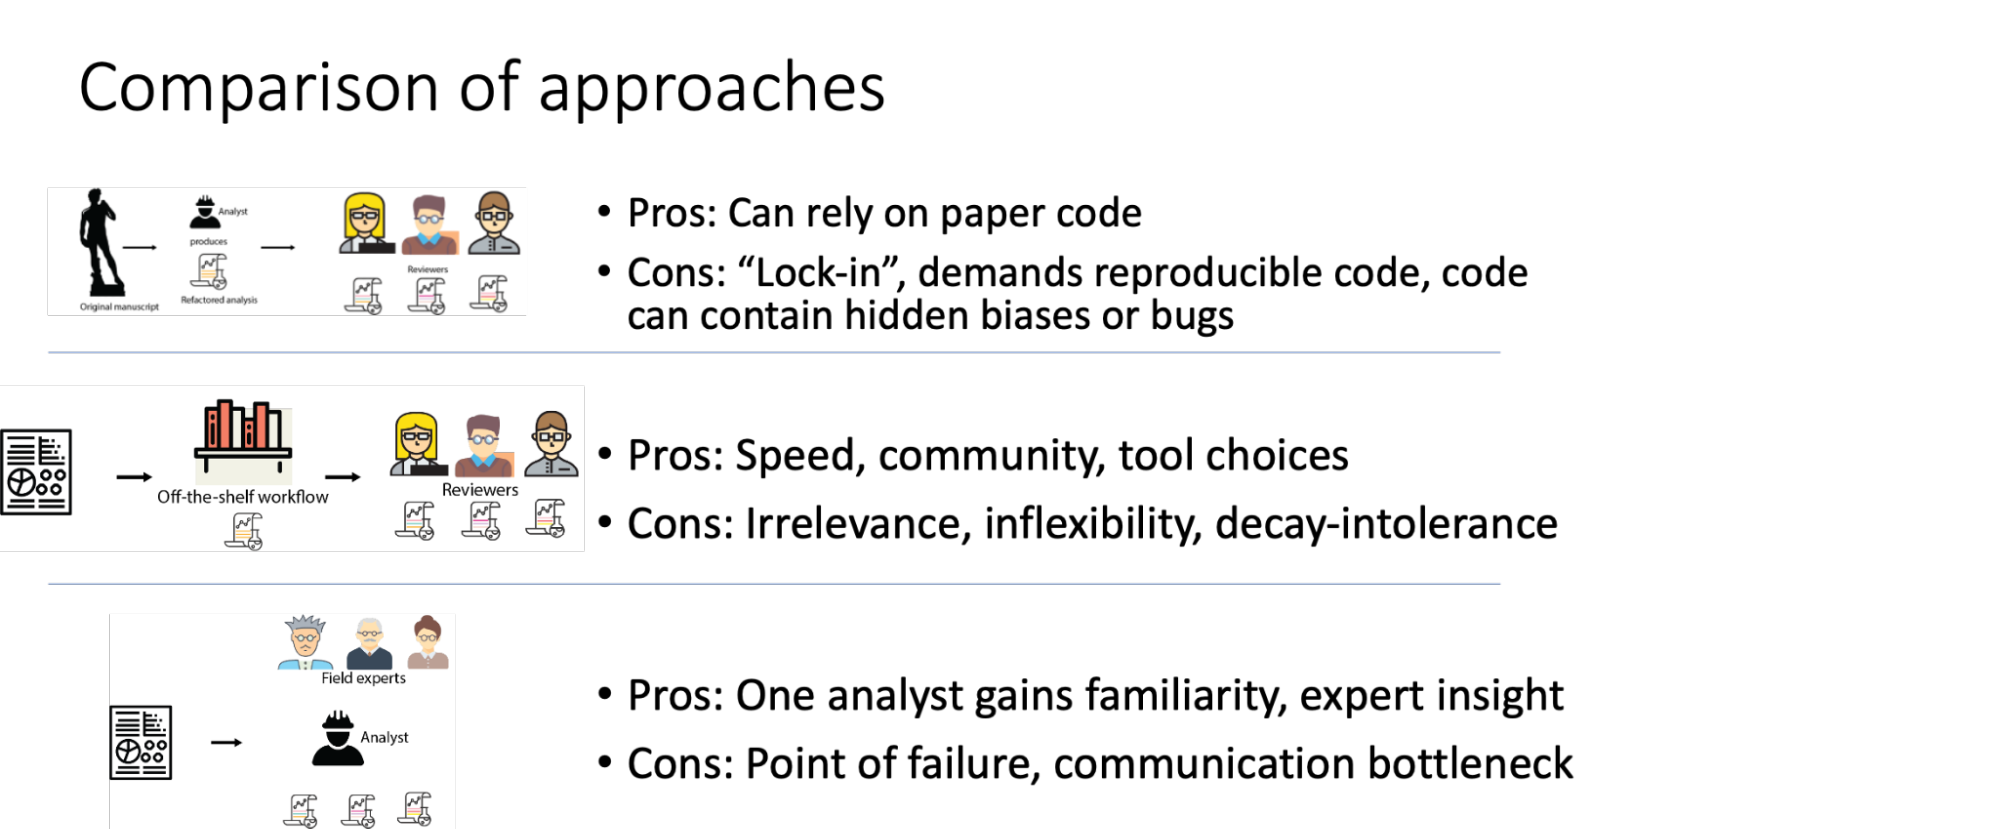
\includegraphics[width=13.76cm,height=5.68cm]{./images/approachcomparison.png}
	\caption{Comparison of approaches}
	\label{approachcomparison}
\end{figure}

The tests of robustness were conducted using three different strategies: refactor alterations, a workflow library, and supervised approaches. Unfortunately, the papers were not round-robin divided among the three approaches. In retrospect, this would have eliminated some of the confounds surrounding this study.

The faithful reproduction and refactor, applied to the Leiby microbiome paper, generated fairly detailed explorations of parameters but little in the way of major tool swaps. In essence, participants did not feel emboldened to completely dismantle the workflow. Some obvious low-hanging fruit would have been major upgrades to Qiime2 or MOTHUR (as opposed to Qiime) and Kraken2 (as opposed to Kraken). None of the participants chose to focus on the metagenomic portions of the analysis.

The workflow library approach was conducted to accelerate the process of evaluation both for the developer and participants and liberate the participants to work in a framework they were familiar with. This approach forced the use of state-of-the-art tools but was not able to directly interrogate all the approaches used by the author as the library of nf-core workflows is wide but not exhaustive. The workflow library approach produced arguably the single most revealing or interesting test of robustness, but that success could be attributed to the talents and aptitude of the reviewer and glaring problems with the original manuscript. In addition to encouraging refactors, this approach can more likely reveal systematic labeling errors and bugs that can remain hidden in existing code submissions and are likely to be missed by reviewers.

The supervised approach posed advantages in terms of having a technician who was familiar with the sample layout combined with senior third-party experts who, while unable to dedicate hours to a test of robustness. In both CLK and m6a these sample metadata and the generation of tool manifests proved very unwieldy, with several combinations of treatments and file types, and posed the single biggest challenge to the quick implementation of refactors. These are not intellectual or scientific challenges but merely data cleaning steps that favor a dedicated professional. In data science circles these data cleaning experts are key members of a data science team, and may someday serve a role in the peer review process.

As tests of robustness are a new concept, communicating the goals to potential reviewers is crucial, as they will have no past exposure to the practice. This study suffered from a lack of communication with some participants, though others were receptive. Packaging of tests of robustness ranged wildly. Reviewers in the Leiby returned essentially intermediates, while reflecting a large number of permutations, were difficult to interpret without taking them downstream. Many participants were understandably reluctant to interpret their findings, not clear if the robustness tests represented support, contradiction, or simply noise.

\subsection{Gaps \& Recommendations}

The following recommendations are derived from the results and discussion above. Some of these recommendations are specifically geared toward the possibility of implementing reproducibility-enabled peer review as a reality, however unlikely, while others are more general guidelines for reproducibility that may prove useful in other contexts.

For clarity, we can organize these along the analytic stack comprised of input data, tools, notebooks/reports, pipelines/workflows, and publications. These correspond to the "analytic stack" discussed in "The Role of Metadata in Reproducible Computational Research" \cite{Leipzig2021-my}.

\begin{figure}[h!]
	\centering
	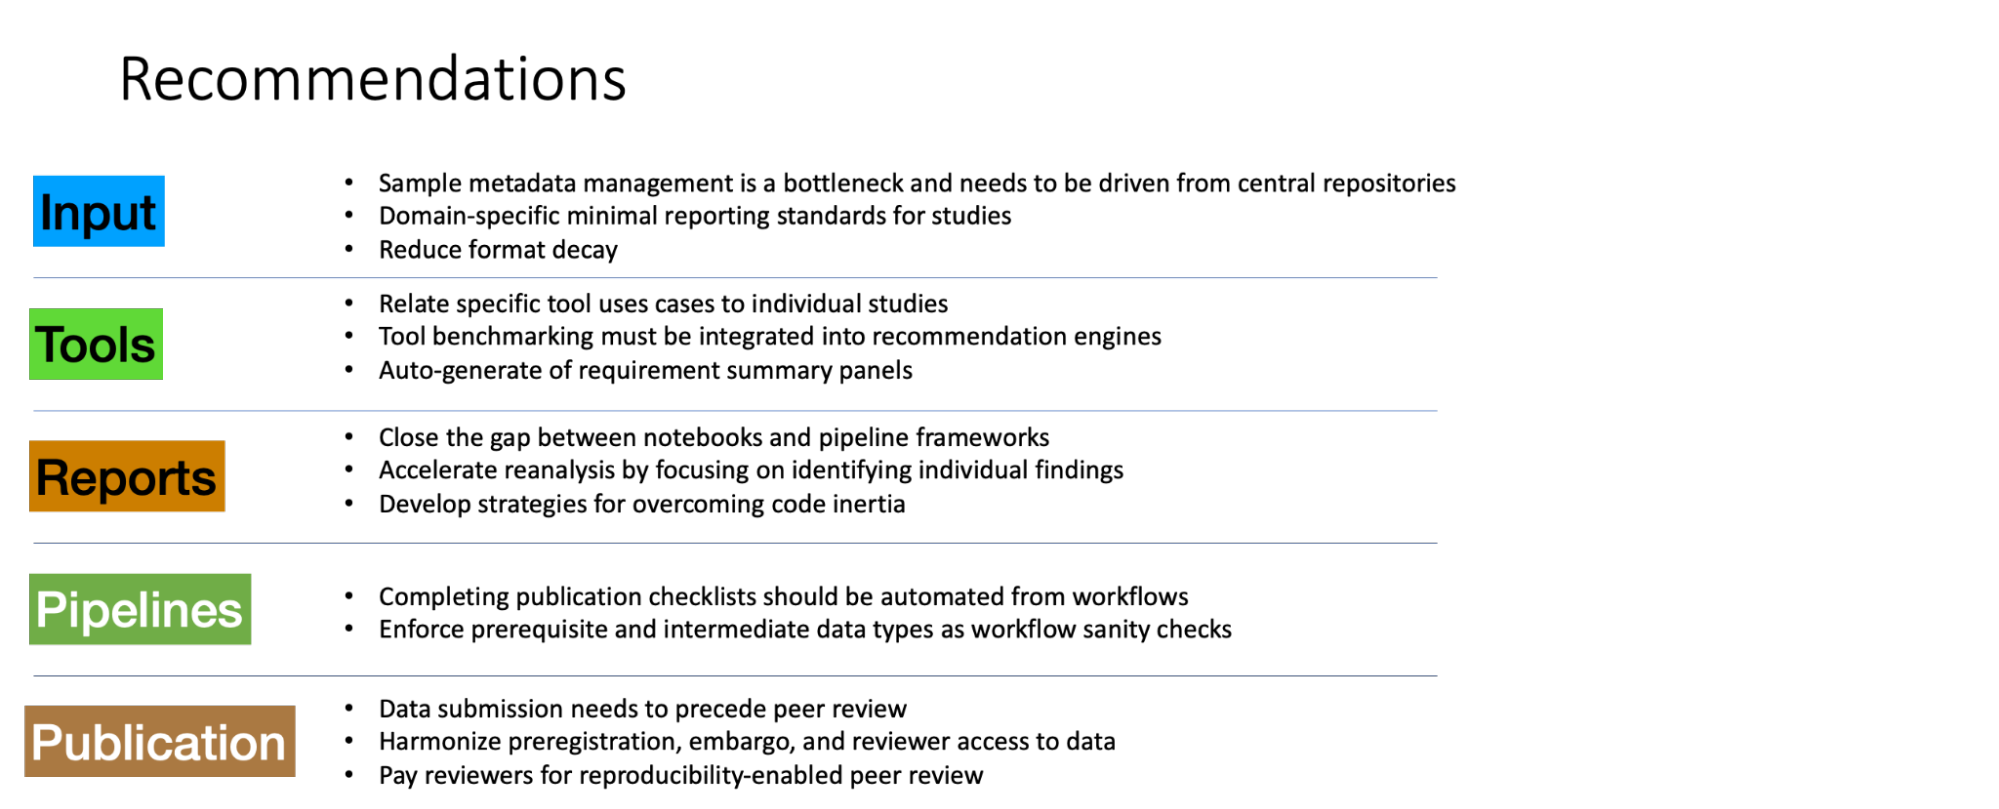
\includegraphics[width=13.76cm,height=6.15cm]{./images/recos.png}
	\caption{High level recommendations for implementing reproducibility-enabled peer review}
	\label{recos}
\end{figure}

\subsubsection{Input data}

\paragraph{Open data / Open code}

For this study it was decided to use papers with no available source code, mostly as a mechanism to learn about what is required to produce a usable study for a test of robustness. In a real-world scenario of peer review, lack of access data or code is unacceptable. As reproducibility standards increase, it seems inevitable that some researchers will attempt to use privacy as a shield against scrutiny. While the public release of identifiable data is a valid concern, there are proper mechanisms for maintaining privacy while enabling reviewers to evaluate analyses that rely on patient data. These can range from mechanisms to isolate data from transfer while allowing inspection and reanalysis to sophisticated cryptographic techniques such as homomorphic encryption \cite{Gursoy2021-fh}.

\paragraph{Domain-specific minimal reporting standards for studies}

All Leiby participants independently reported that a high level of decision entropy, seemingly anecdotal choices in analytic strategy, and associated missing details in free-text methods were defining features of microbiome papers. As a follow-up, Leiby participants were requested to contribute to a checklist specifying "minimal information for a microbiome analysis".


\small{
\onehalfspacing
Minimal Information for a Microbiome Analysis
\begin{itemize}
\item Details on study design
\item The number and type of samples (e.g., strain for animals, demographics for humans)
\item How samples were taken, including inclusion/exclusion criteria if they apply
\item Identity of material being collected
\item How the material was collected, stored, and transported to sequencing
\item Time between data collection and sequencing
\end{itemize}

Minimal data to reproduce a microbiome paper:

\begin{itemize}
\item FASTQs
\item Mapping (samples' metadata) file
\item 16S Database, including clustering identity (e.g. Greengenes clustered at 97$\%$ identity)
\item Taxonomic database (Kraken, kaiju, ...)
\item Annotation database (NCBI-NR, SwissProt, UniProt, kegg mapping, ...)
\item host reference genome (if applied, preferably a link to the same or an upload on zenodo etc.)
\end{itemize}
Minimal list of software/methods to reproduce a microbiome paper:

\begin{itemize}
\item FASTQ primer and low-qual removal software (trimmomatic, cut-adapt, qiime) 
\item FASTQ merge software (pandaseq, vsearch, etc)
\item FASTQ host-filtering process (blast, bwa, bowtie, minimap)
\item 16S "Pipeline" (qiime1, qiime2, dada2, mothur, etc)
\item OTU picking method (uclust, usearch, vsearch, etc)
\item OTU picking strategy (de novo, closed-reference, open-reference)
\item Programs/R libraries to process OTU/ASV tables (phyloseq, etc) and their versions
\item Setting a seed under R or python or other approaches if possible to reproduce the run. 
\item QIIME tracks provenance, so similar information (sessionInfo() from R)
\end{itemize}
Minimal list of analytical steps to report

\begin{itemize}
\item The number of samples included in the final analyses (e.g., those that passed QC)
\item All outcomes-of-interest, and their number (if categorical) or range (if continuous)
\item Details on whether and how outcomes-of-interest are pre-processed
\item How lowly abundant OTUs/ASVs were filtered (called prevalence filtering)
\item Whether and how diversity is measure
\item Whether zeros were imputed or replaced, and how
\item What transformation or normalization procedure was applied
\item The covariates considered to be potential confounders, and criteria used to select them
\item The number and type of statistical tests and presented in the results
\item The number and type of statistical tests performed but not presented in the results
\item The method used to adjust p-values
\end{itemize}

Additional list (other data and methods that should also be included if used):

\begin{itemize}
\item Primers (if not using standard Illumina V3-V4 primers)
\item If Longreads are used, then definitely need the signal level information (either fast5 or subread bams) and the process to generate them. Variation between the various kits used and data quality seems to be improving day by day.
\item Fastq barcode splitter (if FASTQs are barcoded)
\item Taxonomy assignment/classification method
\item Dereplication method
\item Clustering method
\item Chimera removal method
\item Denoise method
\item Assembly method (if not amplicon)
\end{itemize}

All methods should declare program version and parameters used
}
\paragraph{Reducing format decay}

Harmonizing intermediate and final results from comparable software for comparison is essential to robustness tests. First-mover status of certain tools places them to enforce certain output formats, which can take hold. It is inevitable that as a field matures certain new formats will become more accommodating, generalizable, performant, or parsable. This trend places the burden on authors to update their software to support newer formats either as a natively or through a translator. Tool papers often force tool builders to port over older tool results in order to perform benchmarks, but these are essentially isolated or anecdotal incidents. There is no practice, formalized or otherwise, of preventing format decay.

\subsubsection{Tools}

\paragraph{Relating specific tool uses cases to individual studies}

The Funnell CLK paper revealed several unknowns in terms of the predicted behavior of both traditional differential splicing software, isoform discovery and abundance and estimation, and gene fusion detection for conjoined genes in particular. While various free-text searches may reveal appropriate articles, a Google Scholar search of "detection of conjoined genes" is unsatisfactory (and ironically points back to the CLK paper). The difficulty of unknown performance has a profound effect on the potential for reviewers to identify alternative tools to conduct robustness testing quickly.

\paragraph{Potential of recommendation engines for tests of robustness}

One solution to the "tool finding problem" is tool recommendation engines, which associate either manuscript text or workflow provenance traces to patterns of tool usage. This approach has been used extensively in tool recommenders \cite{Palmblad2019-uk}, tool registries \cite{Hillion2017-wg}, and within pipeline frameworks and workflow languages \cite{Bedo2019-ip,Amstutz2015-fa}. In the context of workflows, certain tool combinations tend to be chained in predictable usage patterns driven by application; these patterns can be mined for tool recommender software used in workbenches \cite{Kumar2019-xq}. For better or worse, this reduces the need for workbench developers to manually annotate tools with ontologies, replacing them with a machine learning black box.

\paragraph{Autogeneration of Requirement Summary Panels}

From a reproducible research perspective, it makes sense that these templates should be auto-generated from computational workflows, rather than manually entered. This would require a decorator or tagging scheme by which relevant metadata can be reliably identified even if still embedded as functional variables in workflows. In essence such a schema can guide an entity search engine to easily extract these pertinent details from workflows that conform to a markup standard, thereby saving authors from having to tediously fill out forms but also enabling some freedom of implementation.

\begin{figure}[h!]
	\centering
	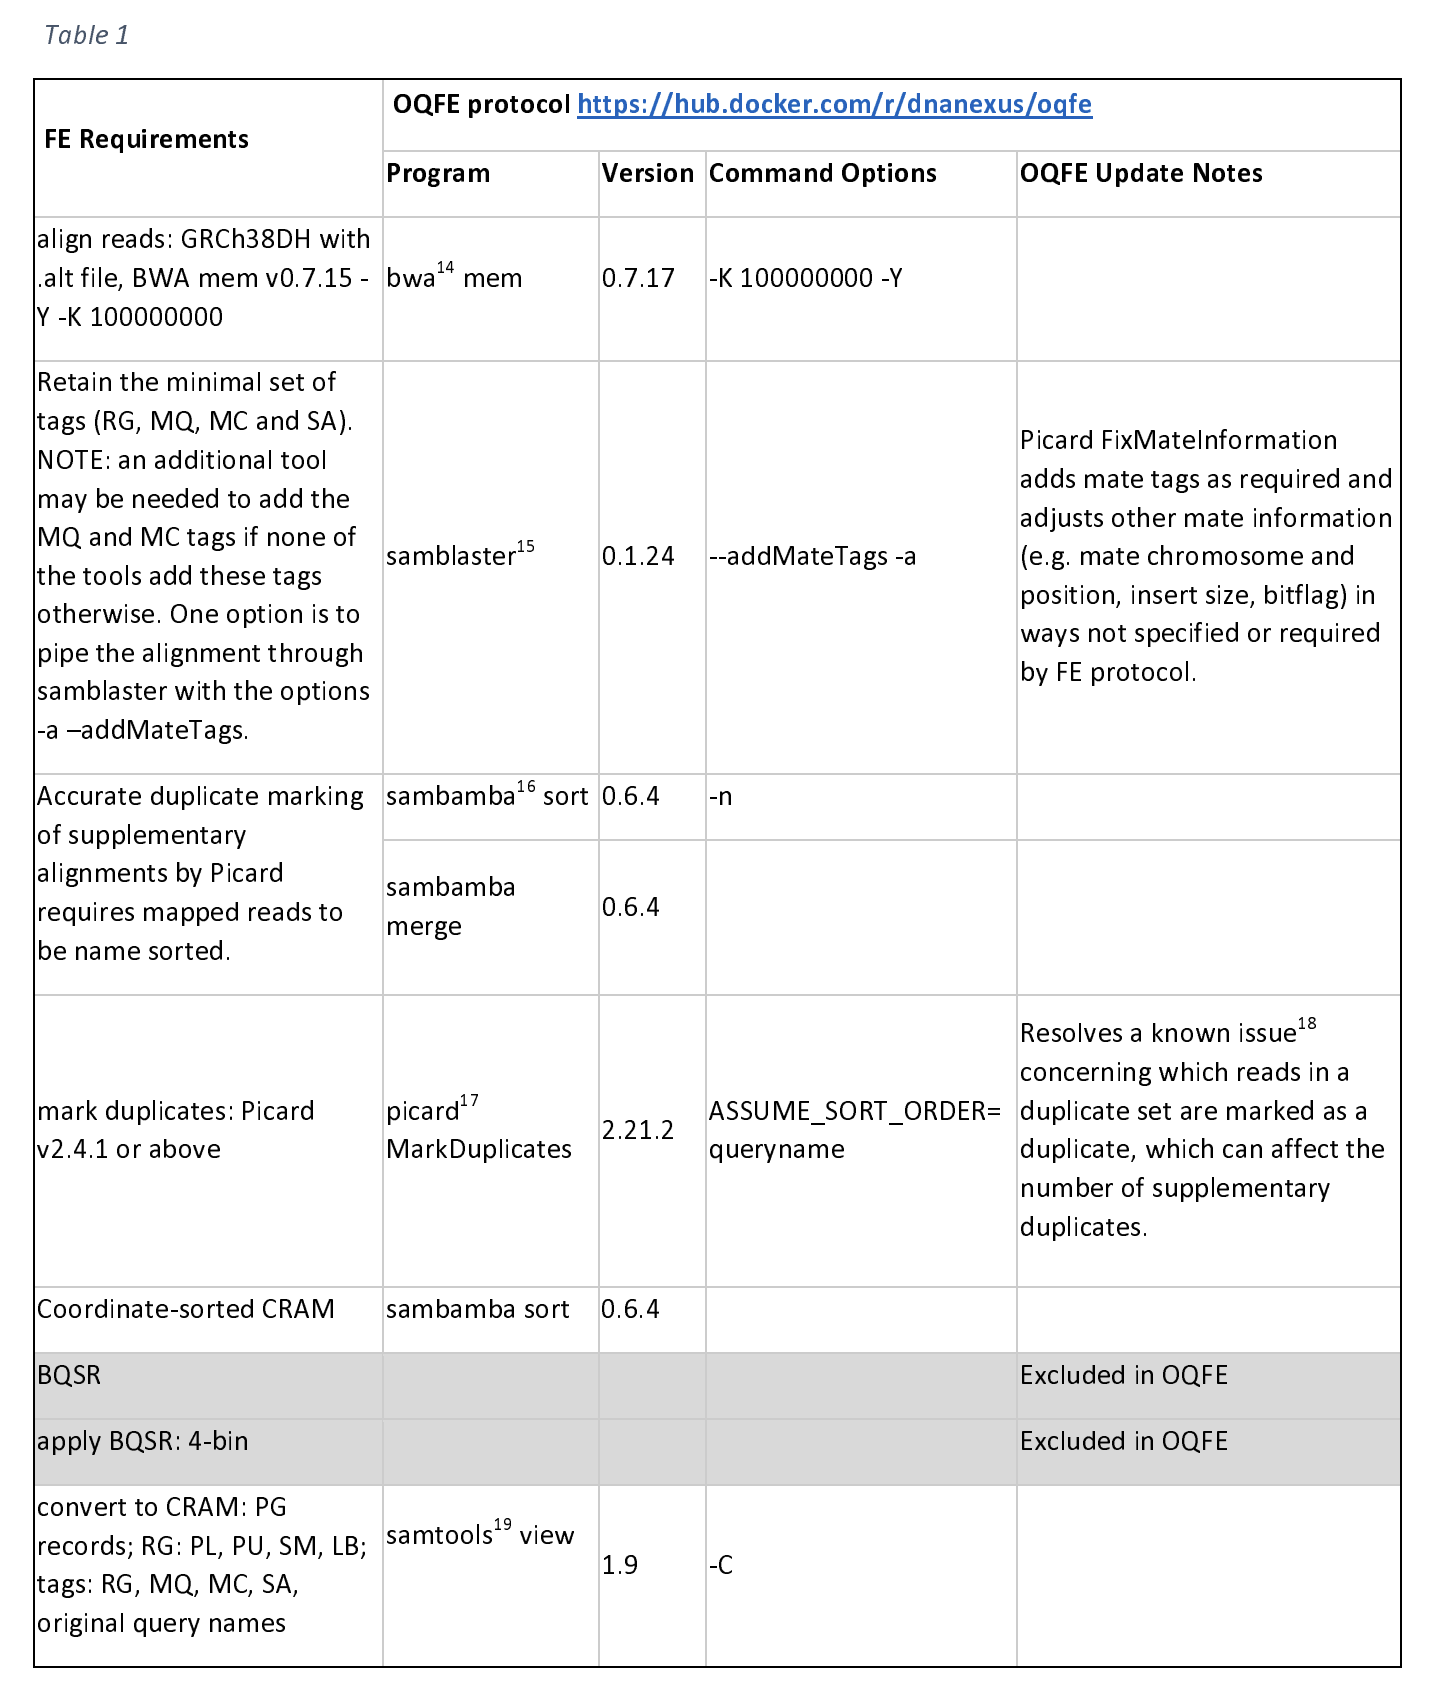
\includegraphics[width=13.76cm,height=16.25cm]{./images/recpanel.png}
	\caption{Requirement summary panel}
	\label{recpanel}
\end{figure}

Requirement summary panels provide a mid-level organized table of a project's software requirements and parameters, existing as a middle conduit between raw code and methods sections. A key feature of these is that not every version and requirement is listed - various secondary and superficial tools would only distract from their pertinence. As of the present, all requirement panels are generated manually for publication, but in most cases it should be possible to autogenerate LaTeX or Markdown formatted panels from dependency management systems, given a domain-specific template.

\subsubsection{Reports \& Notebooks}

\paragraph{Expose resource metadata}

Some steps in the analysis, particularly the building of the Kraken index for Leiby, took many hours to complete. Other tools, such as Mintie, were so slow as to be impractical for high throughput analysis. For the quick dispatch of tests of robustness in the, top level running time and resource specifications CPU/Memory/Running Time estimates for each step of an analysis should be transparently provided.

\paragraph{Adoption of benchmarking frameworks tags into tool sets}

In the case of parameter sweeps, it became quickly clear that Leiby participants were not prepared to design an entire framework for evaluating the results of their changes and simply sent in the code and intermediates they generated instead of collecting metrics. One reason for this is the relative difficulty of building benchmarking frameworks for each such exercise, a problem often experienced in data science where exhaustive hyperparameter exploration of machine learning models is the norm. One possible solution that is emerging is benchmarking frameworks such as Databrick's MLFlow, which integrates with standard programming languages to provide decorator syntax to mark inputs and outputs of interest, where they can be displayed in a local or remotely hosted web interface. The use of benchmarking frameworks is relatively unknown in science, but may provide a means of accelerating robustness testing, especially if prepackaged with tools.

\paragraph{Bridging the gap between notebooks and pipeline frameworks}

Distinguishing high-level choices from low-level details while still permitting that the devil is in the details. Statistical ontology to categorize steps in a workflow that are essentially one of

\begin{itemize}
	\item Group $\&$ matching samples

	\item Removing samples

	\item Normalization

	\item Transformation

	\item Clustering

	\item Glue steps

\end{itemize}
\paragraph{Accelerate reanalysis by focusing on identifying individual findings}

Considerable time was spent in the refactor preparing for downstream or secondary findings that were not examined in the test of robustness. A proper analysis should both prioritize and denote the provenance of results at a high enough level that refactors can 

\paragraph{Increasing the quality and decreasing selective bias of tool benchmarks}

While formal benchmarking projects enable a level playing field for tools to be evaluated, there are opportunities for tool papers to reveal strengths and weaknesses over a range of datasets, rather than a biased training set.

\subsubsection{Pipelines and Workflows}

\paragraph{Automation of publication checklists directly from workflows}

Another important trend is the emergence of reporting guidelines, essentially checklists, many of which are found in the EQUATOR network \cite{Simera2010-cd}, perhaps the most prominent being CONSORT (Consolidated Standards of Reporting Trials) originally from 1996 but updated in 2010 \cite{Schulz2010-bp}. Newer examples include STORMS (Strengthening The Organization and Reporting of Microbiome Studies), Strengthening the Reporting of Observational Studies in Epidemiology (STROBE). Such guidelines, while useful for authors, are rarely paired with metadata schema to allow them to be machine-readable.

\paragraph{Greater enforcement of prerequisite and intermediate data types as workflow sanity checks - the BioSanity project}

Virtually every advance that has improved computational reproducibility in science has been motivated other than pure reproducibility. Dependency managers are largely software development tools, containerization was designed to spin up test instances in e-commerce, literate programming was designed to provide context, notebooks made literate programming interactive,

A common theme that has been presented here is that there is no structured format for understanding or communicating the rationale behind certain tool choices in the context of specific analyses. Bioinformatics still alarmingly relies on folk wisdom mixed in with largely biased tool papers, and a handful of well-conducted benchmarking papers.

The EMBRACE Data And Methods (EDAM) ontology provides high-level descriptions of tools, processes, and biological file formats \cite{Ison2013-gm}. An elegant portal and API for the discovery of omics that utilizes this ontology, bio.tools, allows tool developers to annotate their tools according to common topics, operations, types of data, and data formats. Given its capabilities, bio.tools is an underutilized resource. I have created over 60 bio.tools entries for popular bioinformatic tools that have been in existence for many years, suggesting the bio.tools usage may be low.

Bioinformatic pipelines have become a valued tool to aid reproducibility - as they facilitate the recording of processing and report steps using the incentives of automation, reentrancy, and reuse.

Quality control steps, including those inspecting files directly off of instrumentation and also the output of intermediates and statistical tests, are also an essential part of any solid analysis, but they require manual inspection. 

In an otherwise automated workflow, manual pruning steps create an impediment to reproducibility. Often these are a necessary response to quality control (QC) steps that invalidate certain samples or input data out of the analysis. Removing samples upstream, either by omission or tagging, without any accompanying provenance information informing others of this decision, is a small step away from p-hacking and other undesirable behaviors. Furthermore, this manual step does not address new samples which may be introduced into the analysis or reuse of the pipeline. Most bioinformatics QC software, such as FastQC \cite{Andrews2010-bz} and MultiQC \cite{Ewels2016-uv}, is designed to produce reports but not filter. If a workflow is composed of interpreted steps inside a programming environment, such as R or Python, the task of filtering becomes trivial, but high-throughput analyses are more likely composed of compiled executables run on large files.

Another problem with pipeline frameworks is that they are designed with the assumption that intermediates are suitable as input for the next step, when in fact, they may be corrupt, empty, or insufficient to converge. This weakness allows pipelines to "drive off a cliff" when they encounter such files.

There have been attempts to integrate semantic sanity checks in workflows, namely in WINGS \cite{Zheng2015-qc}, but these have largely focused on self-reported file type rather than edge cases. For example, these solutions only ensure that the reported output of a step is an alignment based on apparent file suffix conventions, but would not validate that the output file consists of more than just a header.

A solution I propose is a sanity checker which dispatches to various bioinformatic utilities (e.g. fastp, samtools, vcftools) to answer basic QC-related assertions:

\begin{verbatim}
./biosanity "is EDAM:format\_1997 and numrecs > 100" --onfail die < myfile
\end{verbatim}

Biosanity will methods typically stored within separate libraries into a common QC-centric focus in a command-line tool. It will feature a limited syntax with basic conditionals and a finite number of reporting or exit strategies to cooperate with various pipeline frameworks. Biosanity will also be a gentle introduction to the use of ontologies for analysts who are not familiar with using them.

\subsubsection{Publication and Peer Review Process}

\paragraph{Develop strategies for overcoming code inertia}

Developers carry an internal conception of how to accomplish tasks, which makes it uncomfortable for them to dive into a stranger's code. In the Dominissini analysis, this tendency was overcome by simply allowing developers to quickly triangulate the paper using off-the-shelf libraries, nf-core. This workflow-library strategy may prove effective only for the most generic of analyses. For robustness testing of newer approaches, original code will have to be used. This limitation could have the undesirable effect of rewarding groups which produce opaque code, avoiding scrutiny through obfuscation. While basic data carpentry can play a role, incentivizing three main requirements, that have been recurrent issues throughout this analysis:

\begin{itemize}
	\item software and dependencies should be installable through Bioconda
    \item pipelines should keep hard-coding parameters to a minimum
    \item samples identifiers both in the manuscript and workflow need to reflect their SRA identifiers
\end{itemize}

\paragraph{Publish with caveats}

One argument against paid peer review is that article processing charges (APCs) are not collected for work that is not accepted, leaving the journal responsible, or that authors would have to pay for each review process at each journal.

\paragraph{Harmonize preregistration, embargo, and reviewer access to data}

A non-trivial issue in the refactors was the use of internal file identifiers to identify samples. While SRA and EBI (the two primary centers for sequence submissions) maintain those names faithfully within uploads, the key identifier is always the SRR or "Run Accession". At present, upload of sequences to SRA is often a later step taken during manuscript submission, only required for final publication.

Ideally, data should be made available to reviewers in the same way that readers will encounter if they choose to reproduce the paper. This ensures that reproducibility is not lost before publication, that data is in fact released (because it needs to be deposited for reviewers before submission), and that centralized quality control can be conducted by repositories that handle the greatest number of sequences.

A minor controversy erupted when it was revealed that a meta-analysis \cite{Edgar2021-lv} had redistributed data that had been mistakenly released by The Jackson Laboratory due to misconfigured changes in embargo period policy. It was revealed that 14,857 data sets were under embargo.

\paragraph{Standardization of cohort-dependent intermediates}

Some analyses with sensitive or identifable data will supply deidentified intermediates, rather than raw data. In other instances, a data point may be tangentially or indirectly rely on private data. One example of private-by-association is the dependence on large identifiable genomic cohorts used in joint genotyping. Obtaining enough statistical signals that indicate a variant is artifactual (strand bias, call quality, mapping quality, max depth), requires several data points to achieve predictive ability under a Bayesian framework (a prior). Additional samples provide more statistical power to infer a variant is due to artifacts. Conversely, obtaining enough evidence that a variant is real also requires more data, only obtainable from additional samples. Sequencing artifacts are highly variable, instrument and library construction, and often specific to individual runs. While cohort-dependent files will never achieve the same level of provenance that standard references or primary data, developing a system of reliably identifying cohorts is essential to the assessment of bias in peer review.

\subparagraph{Paying for reproducibility-enabled peer review}

The concept of compensating peer reviewers for their time and effort is not new - and was a common practice before 1980. A recent proposal, the $\$$450 Movement, has garnered the attention of the broader scientific community \cite{noauthor_2021-ok} and has spawned a debate over the feasibility, ethics, and possible side-effects of this idea have been discussed in several forums \cite{Vines2021-bh}. Reproducibility and the replication crisis are often discussed hand-in-hand with paid peer review - the gist being that terse or low-quality reviews are at least in part responsible for the proliferation of irreproducible results. Virtually none of this discussion has focused specifically on reproducibility-enabled in silico peer review. The typical peer review takes 5 hours to complete \cite{Mark_Ware2015-bx}. While participants in this thesis project were not asked how many hours they spent on their analyses, direct personal communications with several participants in the unsupervised refactor and workflow library groups indicate at least 20 hours were required to complete this task. A casual twitter poll was conducted for this thesis to gauge what authors would "expect for their money," of the 585 votes, improvement in turnaround speed (70.4$\%$), length or comprehensiveness of reviews (19.1$\%$), help with English (2.2$\%$), and help with analysis (8.2$\%$).

\paragraph{Improving conceptual-level DAGs}

The ENCODE portal \cite{Hong2016-en} provides some of the best DAGs in the form of high-level association graphs, and these tend to be more understandable than the "spaghetti" DAGs. The use of such conceptual DAGs may help distinguish provenance from lower-level noise.

\begin{figure}[h!]
	\centering
	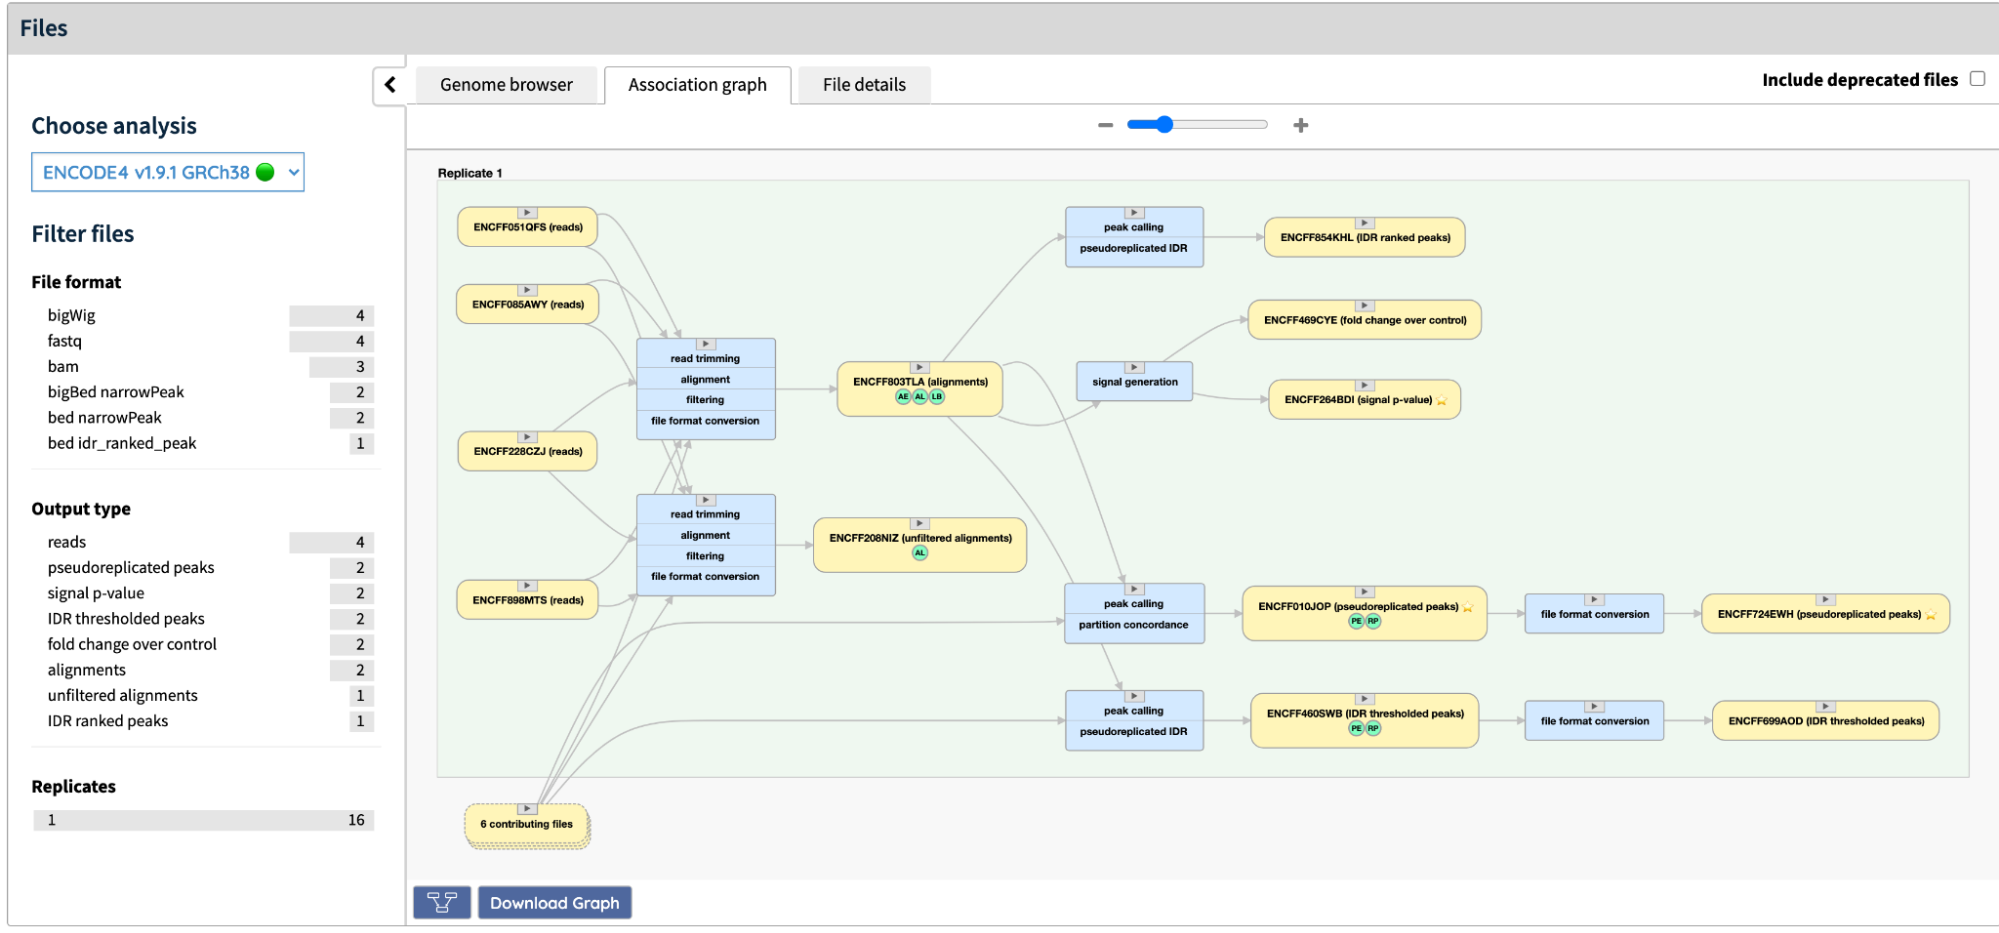
\includegraphics[width=13.76cm,height=6.38cm]{./images/encode.png}
	\caption{ENCODE portal directed acyclic graphs for processes}
	\label{encode}
\end{figure}

ENCODE portal directed acyclic graphs for processes

\subsubsection{Applicable Metadata Standards}

The review paper "The Role of Metadata in Reproducible Computational Research" exhaustively compiled a list of applicable metadata standards for reproducible research. Some of these standards appear applicable to tests of robustness. 

\begin{table}[H]
\begin{adjustbox}{max width=\textwidth}
\begin{tabular}{p{4.07cm}p{2.67cm}p{9.82cm}p{4.07cm}p{2.67cm}p{9.82cm}}
\hline
\multicolumn{1}{|p{4.07cm}}{Tool} & 
\multicolumn{1}{|p{2.67cm}}{Type of Standard} & 
\multicolumn{1}{|p{9.82cm}|}{Description} \\ 
\hline
\multicolumn{1}{|p{4.07cm}}{BioCompute Objects\cite{Simonyan2017-st}} & 
\multicolumn{1}{|p{2.67cm}}{Workflow } & 
\multicolumn{1}{|p{9.82cm}|}{Provides lab and runtime parameter standards for workflows and tools} \\ 
\hline
\multicolumn{1}{|p{4.07cm}}{GoGetData} & 
\multicolumn{1}{|p{2.67cm}}{Data} & 
\multicolumn{1}{|p{9.82cm}|}{Data as a dependency tool} \\ 
\hline
\multicolumn{1}{|p{4.07cm}}{EDAM\cite{Ison2013-gm}} & 
\multicolumn{1}{|p{2.67cm}}{Tool} & 
\multicolumn{1}{|p{9.82cm}|}{Bioinformatic tool ontology} \\ 
\hline
\multicolumn{1}{|p{4.07cm}}{BioConda\cite{Dale2017-aj}} & 
\multicolumn{1}{|p{2.67cm}}{Tool} & 
\multicolumn{1}{|p{9.82cm}|}{Dependency resolution} \\ 
\hline
\multicolumn{1}{|p{4.07cm}}{labelschema} & 
\multicolumn{1}{|p{2.67cm}}{Tool} & 
\multicolumn{1}{|p{9.82cm}|}{Docker label metadata standard} \\ 
\hline
\multicolumn{1}{|p{4.07cm}}{Common Workflow Language\cite{Peter2016-vi}} & 
\multicolumn{1}{|p{2.67cm}}{Workflow } & 
\multicolumn{1}{|p{9.82cm}|}{pipeline framework language } \\ 
\hline
\multicolumn{1}{|p{4.07cm}}{Workflow Description Language\cite{Voss2017-ro}} & 
\multicolumn{1}{|p{2.67cm}}{Workflow } & 
\multicolumn{1}{|p{9.82cm}|}{pipeline framework language} \\ 
\hline
\multicolumn{1}{|p{4.07cm}}{Drake\cite{Landau_undated-yt}} & 
\multicolumn{1}{|p{2.67cm}}{Analysis} & 
\multicolumn{1}{|p{9.82cm}|}{Analysis pipeline framework} \\ 
\hline
\multicolumn{1}{|p{4.07cm}}{OBCS\cite{Zheng2016-cu}} & 
\multicolumn{1}{|p{2.67cm}}{Analysis} & 
\multicolumn{1}{|p{9.82cm}|}{Statistical ontology} \\ 
\hline
\multicolumn{1}{|p{4.07cm}}{CodeMeta\cite{Jones2016-dz}} & 
\multicolumn{1}{|p{2.67cm}}{Analysis} & 
\multicolumn{1}{|p{9.82cm}|}{Code metadata standard} \\ 
\hline
\multicolumn{1}{|p{4.07cm}}{Bagit\cite{Kunze2018-pn}} & 
\multicolumn{1}{|p{2.67cm}}{Analysis} & 
\multicolumn{1}{|p{9.82cm}|}{Analysis file archival standard} \\ 
\hline
\multicolumn{1}{|p{4.07cm}}{ReproZip\cite{Simonyan2017-st}} & 
\multicolumn{1}{|p{2.67cm}}{Analysis} & 
\multicolumn{1}{|p{9.82cm}|}{Analysis file archival standard} \\ 
\hline
\multicolumn{1}{|p{4.07cm}}{DataPackageR\cite{Finak2018-ai}} & 
\multicolumn{1}{|p{2.67cm}}{Analysis} & 
\multicolumn{1}{|p{9.82cm}|}{Analysis archival standard} \\ 
\hline
\multicolumn{1}{|p{4.07cm}}{Binder\cite{Jupyter2018-md}} & 
\multicolumn{1}{|p{2.67cm}}{Analysis} & 
\multicolumn{1}{|p{9.82cm}|}{Containerized notebook live viewer} \\ 
\hline
\multicolumn{1}{|p{4.07cm}}{YesWorkflow\cite{McPhillips2015-um}} & 
\multicolumn{1}{|p{2.67cm}}{Analysis} & 
\multicolumn{1}{|p{9.82cm}|}{Analysis pipeline markup} \\ 
\hline
\multicolumn{1}{|p{4.07cm}}{Manubot\cite{Himmelstein2019-dt}} & 
\multicolumn{1}{|p{2.67cm}}{Publication} & 
\multicolumn{1}{|p{9.82cm}|}{Automated git-driven publications} \\ 
\hline
\multicolumn{1}{|p{4.07cm}}{RRID\cite{Bandrowski2015-qu}} & 
\multicolumn{1}{|p{2.67cm}}{Publication} & 
\multicolumn{1}{|p{9.82cm}|}{Resource tags for papers} \\ 
\hline
\multicolumn{1}{|p{4.07cm}}{Research Objects\cite{Bechhofer2010-lr}} & 
\multicolumn{1}{|p{2.67cm}}{Publication } & 
\multicolumn{1}{|p{9.82cm}|}{Metadata describing and bundling the entire experiment} \\ 
\hline
\end{tabular}
\end{adjustbox}
\caption{Tools and metadata supporting reproducible research}
\end{table}

\subsection{Conclusion}

This dissertation investigates the feasibility of using tests of robustness in the context of reproducibility enabled \textit{in silico} peer review. Tests of robustness involve manipulating software tools, parameters, and statistical models with the intention of evaluating the underlying validity of an existing analysis. This practice is presented as a natural extension of technological advances in the last 5 years combined with growing awareness and case studies of reproducibility and issues of scientific quality.

The research problem was investigated through a unique human research mixed-model in which participants were engaged in the reproducibility-enabled peer review process, either actively or expert advisors, using high-impact genomic manuscripts selected to elicit review findings. Pre- and post-hoc surveys were also conducted to measure attitudes about reproducibility and the tests of robustness. The development of the materials for these tests, bioinformatic pipelines which I designed, were also explicitly intended to evaluate the process. This practice of refactoring papers without source code demonstrated many weaknesses of conventional scientific publishing standards.

Three papers - on the microbiome, m6a methylation, and CLK-induced splicing changes were approached by different means as difficulties and opportunities revealed themselves. It was discovered, perhaps not surprisingly, that reviewers would be reluctant to manipulate complex pipelines beyond parameter exploration to overhauls of core tools, and so findings were limited to such parameter sweeps and were largely inconclusive. A workflow library approach was conducted for the m6a paper, by which participants were asked to use off-the-shelf pipelines to triangulate the inspection of a paper with known problems. The workflow library approach appeared ostensibly more successful than the other approaches, though the paper choice remained a confounding factor. The final paper involved a mixed exotic combination of both long and short reads and an unusual phenotype - conjoined genes, making it better suited toward attempting swaps with the latest tools. Experts were consulted, and I performed the tests of robustness independently. Some of these tests might have proven useful if they were conducted at the time of peer review.

\subsection{Material Outcomes}

Prior to this proposal, I composed a review article, book chapter, an online case study catalog, and finally, a prospectus that set the foundation for some of the ideas described in this proposal. In "A Review of Bioinformatic Pipeline Frameworks" \cite{Leipzig2017-hv}, I attempted to classify existing software solutions for handling serial and parallel abstracted bioinformatic workflows to process sequence data and metadata. This review contends that existing frameworks differ on three key dimensions: using an implicit or explicit syntax, using a configuration, convention, or class-based design paradigm, and offering a command line or workbench interface. While not an absolute requirement for computational reproducibility, the use of pipeline frameworks encourages reproducible research by abstracting file transformation steps into a parameterized and configured sequence. Such frameworks offer cohesion between tools and data and analysis and encourage reuse and robustness through the advantages of easy extensibility and scalability, particularly through the cloud. As of this date, the review has received 257 citations.

A follow-up to this review is the book chapter "Computational Pipelines and Workflows in Bioinformatics" \cite{Leipzig2019-ag}. In this review I explored the ecosystem that has evolved around workflows - toolkits, ready-made pipelines, and pipeline frameworks. Future directions of dependency management and configuration, cloud computing, containerization, and notebooks. Of particular relevance to this is a discussion into the possibilities of semantically encoded workflows and linked data, including existing solutions built on the PROV-O ontology \cite{Belhajjame2013-at,Missier2013-ea}. A discussion on the difficulties of encoding and binding upstream experimental metadata to end results that emerged from this chapter informs much of this proposal.

The Role of Metadata in Reproducible Computational Research, exhaustively explores metadata standards that are applicable to reproducible computational research, organized with respect to the analytic stack, and accompanied by numerous source code examples. It was accepted into Cell Patterns for an August 2021 edition. It has received ten citations.

Awesome Reproducible Research \cite{Leipzig2019-am} is a Github repository storing my research into case studies and other reproducible research resources that I have collected over my studies. It has 183 stars and has received contributions from 9 users.

\newpage

\printbibliography

\section{Appendix}

\subsection{General Survey Responses}

See \url{https://figshare.com/articles/dataset/Survey_responses/17054270} for full survey responses.

\subsection{Individual Reports}

\subsubsection{Leiby et al.}

The Leiby et al refactor and links to individual participant reports are available at: \url{https://github.com/leipzig/placenta}.

\subsubsection{Dominissini et al.}
The Nextflow templates, manifest generator and links to the Dominissini et al reports are available at \url{https://github.com/leipzig/m6a}.

\subsubsection{Funnell et al.}
The tests of robustness performed for Funnell et al are available at \url{https://github.com/leipzig/clk}.

\newpage

\section{Vita}

Jeremy Leipzig

\subsection{Education}

Wake Forest University – Bachelor of Science in Biology 1997

North Carolina State University – Master of Computer Science 2003

\subsection{Publications}

\textbf{Leipzig, J}.; Nüst, D.; Hoyt, C. T.; Ram, K.; Greenberg, J. The Role of Metadata in Reproducible Computational Research. Cell Patterns, 2021.

\textbf{Leipzig, J}.; Bakis, Y.; Wang, X.; Elhamod, M.; Diamond, K.; Dahdul, W.; Karpatne, A.; Maga, M.; Mabee, P.; Bart, H. L.; Greenberg, J. Biodiversity Image Quality Metadata Augments Convolutional Neural Network Classification of Fish Species. \textit{Cold Spring Harbor Laboratory}, 2021, 2021.01.28.428644.

Elhamod, M.; Diamond, K. M.; Maga, A. M.; Bakis, Y.; Bart, H. L.; Mabee, P.; Dahdul, W.; \textbf{Leipzig, J}.; Greenberg, J.; Avants, B.; Others. Hierarchy-Guided Neural Networks for Species Classification. \textit{bioRxiv} \textbf{2021}.

Raman, P.; Zimmerman, S.; Rathi, K. S.; de Torrent, L.; Sarmady, M.; Wu, C.; \textbf{Leipzig, J.}; Taylor, D. M.; Tozeren, A.; Mar, J. C. A Comparison of Survival Analysis Methods for Cancer Gene Expression RNA-Sequencing Data. Cancer Genet. 2019, 235-236, 1–12.

McManus, M. J.; Picard, M.; Chen, H.-W.; De Haas, H. J.; Potluri, P.;\textbf{ Leipzig, J.}; Towheed, A.; Angelin, A.; Sengupta, P.; Morrow, R. M.; Kauffman, B. A.; Vermulst, M.; Narula, J.; Wallace, D. C. Mitochondrial DNA Variation Dictates Expressivity and Progression of Nuclear DNA Mutations Causing Cardiomyopathy. Cell Metab. 2019, 29 (1), 78–90.e5.

\textbf{Leipzig, J.} Computational Pipelines and Workflows in Bioinformatics. In Reference Module in Life Sciences; Elsevier, 2018.

Sonney, S.; \textbf{Leipzig, J.}; Lott, M. T.; Zhang, S.; Procaccio, V.; Wallace, D. C.; Sondheimer, N. Predicting the Pathogenicity of Novel Variants in Mitochondrial tRNA with MitoTIP. PLoS Comput. Biol. 2017, 13 (12), e1005867.

Chalkia, D.; Singh, L. N.; \textbf{Leipzig, J.}; Lvova, M.; Derbeneva, O.; Lakatos, A.; Hadley, D.; Hakonarson, H.; Wallace, D. C. Association Between Mitochondrial DNA Haplogroup Variation and Autism Spectrum Disorders. JAMA Psychiatry 2017 DOI: 10.1001/jamapsychiatry.2017.2604.

\textbf{Leipzig, J.} (2017). A review of bioinformatic pipeline frameworks. Briefings in Bioinformatics. 2016 10.1093/bib/bbw020

Navarro-Gomez D, \textbf{Leipzig J,} Shen L, Lott M, Stassen AP, Wallace DC, Wiggs JL, Falk MJ, van Oven M, Gai X. Phy-Mer: a novel alignment-free and reference-independent mitochondrial haplogroup classifier. Bioinformatics. 2014 Dec 12. 10.1093/bioinformatics/btu825

Falk MJ, Shen L, Gonzalez M, \textbf{Leipzig J,} Lott MT, Stassen AP, Diroma MA, Navarro-Gomez D, Yeske P, Bai R, Boles RG, Brilhante V, Ralph D, DaRe JT, Shelton R, Terry SF, Zhang Z, Copeland WC, van Oven M, Prokisch H, Wallace DC, Attimonelli M, Krotoski D, Zuchner S, Gai X. Mitochondrial Disease Sequence Data Resource (MSeqDR): A global grass-roots consortium to facilitate deposition,curation, annotation, and integrated analysis of genomic data for the mitochondrial disease clinical and research communities. Mol Genet Metab. 2014 Dec 4. pii: S1096-7192(14)00377-1.

Glessner JT, Bick AG, Ito K, Homsy JG, Rodriguez-Murillo L, Fromer M, Mazaika E, Vardarajan B, Italia M, \textbf{Leipzig J}, DePalma SR, Golhar R, Sanders SJ, Yamrom B, Ronemus M, Iossifov I, Willsey AJ, State MW, Kaltman JR, White PS, Shen Y, Warburton D, Brueckner M, Seidman C, Goldmuntz E, Gelb BD, Lifton R, Seidman J, Hakonarson H, Chung WK. Increased frequency of de novo copy number variants in congenital heart disease by integrative analysis of single nucleotide polymorphism array and exome sequence data. Circ Res. 2014 Oct 24;115(10):884-96.

Lott MT, \textbf{Leipzig JN}, Derbeneva O, Xie HM, Chalkia D, Sarmady M, Procaccio V, Wallace DC. mtDNA Variation and Analysis Using MITOMAP and MITOMASTER. Curr Protoc Bioinformatics. 2013 Dec 12;1(123):1.23.1-1.23.26

Zaidi, S., Choi, M., Wakimoto, H., Ma, L., Jiang, J., Overton, J. D., et al. De novo mutations in histone-modifying genes in congenital heart disease. Nature 498, 220–223

Zhang Z, \textbf{Leipzig J}, Sasson A, Perin JC, Xie M, Sarmady M, Warren P, White P. Digest of high-throughput sequencing in a reproducible report. BMC Bioinformatics. 2013, 14(Suppl 11):S3.

Barrantes I, \textbf{Leipzig J}, Marwan W. A next-generation sequencing approach to study the transcriptomic changes during the differentiation of physarum at the single-cell level. Gene Regul Syst Bio. 2012;6:127-37.

Shi L, Perin JC, \textbf{Leipzig J}, Zhang Z, Sullivan KE. Genome-wide analysis of interferon regulatory factor I binding in primary human monocytes. Gene. 2011 Nov 1;487(1).

\textbf{Leipzig J,} Li Xiao-Yi. Data Mashups in R. O’Reilly. 2009. (Reissued in 2011)

Wang GP, Garrigue A, Ciuffi A, Ronen K, \textbf{Leipzig J}, Berry C, Lagresle-Peyrou C, Benjelloun F, Hacein-Bey-Abina S, Fischer A, Cavazzana-Calvo M, Bushman FD. DNA barcoding and pyrosequencing to analyze adverse events in therapeutic gene transfer. Nucleic Acids Res. 2008 May;36(9):e49.

Meekings KN, \textbf{Leipzig J}, Bushman FD, Taylor GP, Bangham CR.HTLV-1 integration into transcriptionally active genomic regions is associated with proviral expression and with HAM/TSP. PLoS Pathog. 2008 Mar 21;4(3):e1000027.

Hoffmann C, Minkah N, \textbf{Leipzig J}, Wang G, Arens MQ, Tebas P, Bushman FD. DNA bar coding and pyrosequencing to identify rare HIV drug resistance mutations. Nucleic Acids Res. 2007;35(13):e91.

Wang GP, Ciuffi A, \textbf{Leipzig J}, Berry CC, Bushman FD. HIV integration site selection: analysis by massively parallel pyrosequencing reveals association with epigenetic modifications. Genome Res. 2007 Aug;17(8):1186-94.

Berry C, Hannenhalli S, \textbf{Leipzig J}, Bushman FD. Selection of target sites for mobile DNA integration in the human genome. PLoS Comput Biol. 2006 Nov 24;2(11):e157.

Lewinski MK, Yamashita M, Emerman M, Ciuffi A, Marshall H, Crawford G, Collins F, Shinn P,\textbf{ Leipzig J}, Hannenhalli S, Berry CC, Ecker JR, Bushman FD. Retroviral DNA integration: viral and cellular determinants of target-site selection. PLoS Pathog. 2006 Jun;2(6):e60.

Barr SD, Ciuffi A, \textbf{Leipzig J}, Shinn P, Ecker JR, Bushman FD. HIV integration site selection: targeting in macrophages and the effects of different routes of viral entry. Mol Ther. 2006 Aug;14(2):218-25.

Ciuffi A, Mitchell RS, Hoffmann C, \textbf{Leipzig J}, Shinn P, Ecker JR, Bushman FD. Integration site selection by HIV-based vectors in dividing and growth-arrested IMR-90 lung fibroblasts.Mol Ther. 2006 Feb;13(2):366-73.

Ciuffi A, Llano M, Poeschla E, Hoffmann C, \textbf{Leipzig J}, Shinn P, Ecker J, Bushman F. A role for LEDGF/p75 in targeting HIV DNA integration.Nat Med. 2005 Dec;11(12):1287-9.

Bushman F, Lewinski M, Ciuffi A, Barr S, \textbf{Leipzig J}, Hannenhalli S, Hoffmann C. Genome-wide analysis of retroviral DNA integration. Nat Rev Microbiol. 2005 Nov;3(11):848-58.

Barr SD, \textbf{Leipzig J}, Shinn P, Ecker JR, Bushman FD. Integration targeting by avian sarcoma-leukosis virus and human immunodeficiency virus in the chicken genome. J Virol. 2005 Sep;79(18):12035-44.

\textbf{Leipzig J}, Pevzner P, Heber S. The Alternative Splicing Gallery (ASG): bridging the gap between genome and transcriptome. Nucl. Acids. Res. 2004 32: 3977-3983.

Duncan GE, Miyamoto S,\textbf{ Leipzig JN}, Lieberman JA. Comparison of the effects of clozapine, risperidone, and olanzapine on ketamine-induced alterations in regional brain metabolism.J Pharmacol Exp Ther. 2000 Apr;293(1):8-14.

Miyamoto S, \textbf{Leipzig JN}, Lieberman JA, Duncan GE. Effects of ketamine, MK-801, and amphetamine on regional brain 2-deoxyglucose uptake in freely moving mice. Neuropsychopharmacology. 2000 Apr;22(4):400-12.

Duncan GE, Miyamoto S, \textbf{Leipzig JN}, Lieberman JA. Comparison of brain metabolic activity patterns induced by ketamine, MK-801 and amphetamine in rats: support for NMDA receptor involvement in responses to subanesthetic dose of ketamine. Brain Res. 1999 Oct 2;843(1-2):171-83.

Duncan GE, \textbf{Leipzig JN}, Mailman RB, Lieberman JA. Differential effects of clozapine and haloperidol on ketamine-induced brain metabolic activation. Brain Res. 1998 Nov 23;812(1-2):65-75.



%\begin{appendices}
%\input{appendix_proofs/appendix_introduction.tex}
%\end{appendices}

%\vita{
%Write your back of the book bio there.
%}
%\blankpage

\newpage 

\ % The empty page

\newpage


\end{document}